%\documentclass[../../tesis.tex]{subfiles}
\documentclass[class=article, crop=false]{standalone}
\usepackage[subpreambles=true]{standalone}
\usepackage{import}
\graphicspath{{images/}}


%
%
%
%
\usepackage{amssymb}
\usepackage{amsmath}
%\usepackage{natbib}
\setcounter{tocdepth}{3}
\usepackage{graphicx}
%\graphicspath{ {Graficos/} }
\usepackage{subfigure}
\usepackage{gensymb}
\usepackage{authblk}
\usepackage{url}
\usepackage[utf8]{inputenc}

\usepackage[spanish]{babel}
\selectlanguage{spanish}
%\usepackage[style=authoryear]{biblatex}

\begin{document}

\section{Introducción}

En la presente sección se buscará captar los rasgos generales de la estructura del comercio internacional, con independencia de los productos específicos que los países comercian. Si bien el rol que ocupan los países en la Nueva División Internacional del Trabajo determina a la vez qué tipo de mercancías concentran su producción para el mercado mundial y la importancia que tienen los mismos en dicha red \citep{frobel1978new}, esto no quita el valor de analizar la centralidad de los países, con independencia de las ramas en que cada país concentra sus exportaciones e importaciones. Naturalmente, los resultados de dicho análisis son representan una caracterización que puede resultar útil como complemento para estudios que indaguen respecto de las causas de dicha distribución.

En la literatura reciente se realizaron diversos enfoques desde esta perspectiva, ya sea desde una mirada de la teoría de la información \cite{Bhattacharya2008},  como una herramienta de modelización de los fenómenos económicos \cite{Fan2014}, para analizar las relaciones de centro-periferia \cite{Fagiolo2010}, o bien para realizar una descripción del estado del comercio internacional \cite{Chow2013}. Sin embargo, dada la amplitud de los temas a abordar, tanto desde la perspectiva económica, como desde la teoría de grafos, se presenta como un campo abierto para la investigación, con sendas aristas aún por recorrer.        

El capítulo se estructura de la siguiente manera: En la sección siguiente se realiza un análisis exploratorio de datos, mientras que la sección tercera describe las fuentes de información utilizadas y realiza un pequeño resumen de los elementos de la teoría de grafos utilizados, así como las particularidades que surgen al aplicar esta marco metodológico al comercio internacional. La sección cuarta presenta los resultados, con detalle en el año 2016, así como también un análisis de mediano y largo plazo de la evolución de la red. Finalmente, se presentan las conclusiones específicas a este capítulo.


\section{Análisis Exploratorio de Datos}


En primer lugar, en la figura \ref{fig:rel_dep-1}, analizamos la frecuencia de las interacciones entre países en función de la proporción del comercio que representan para el país importador. La distribución tiene una asimetría a derecha, que asemeja una distribución de chi-cuadrado. En la figura \ref{fig:rel_dep-1} se puede observar que si bien la gran mayoría de las relaciones bilaterales de comercio representan una baja proporción de las importaciones de un determinado país, existen ciertas relaciones comerciales que se podrían caracterizar como de alta dependencia para el país importador. 
En particular, se observan cuatro relaciones comerciales de alta dependencia para el año 2016: La venta de mercancías de Estados Unidos a las islas de San Cristóbal y Nieves y Bermudas ; las exportaciones de Dinamarca a Groenlandia y de la India a Nepal. 

En la figura \ref{fig:rel_dep-2} se puede observar aquellas relaciones que representan más de un 70\% de las importaciones del país importador, para el período 1996-2017. Allí se destaca con el tamaño de fuente el Valor comerciado en cada dupla para cada año en particular. La mayoría de las relaciones de tipo dependiente se repiten año a año y constituyen volúmenes bajos de comercio, entre países de tamaños, económicos poblacionales y territoriales, muy diferentes entre sí. En particular destaca Estados Unidos en su relación comercial con pequeñas islas del Caribe, y Sudáfrica con países de menor tamaño en su mismo continente, como Namibia o Botswana. Otra relación de comercio dependiente que se repite en la serie es la exportación de productos desde Israel a Palestina. Sin embargo, todas estas relaciones implican un monto menor en términos del comercio mundial. La relación de tipo dependiente más importante es la exportación de productos desde Estados Unidos hacia México durante la década del noventa, en el proceso conocido como la "maquila mexicana" \citep{carrillo1998third}


\begin{figure}
	\centering
	\subfigure[2016]{\label{fig:rel_dep-1}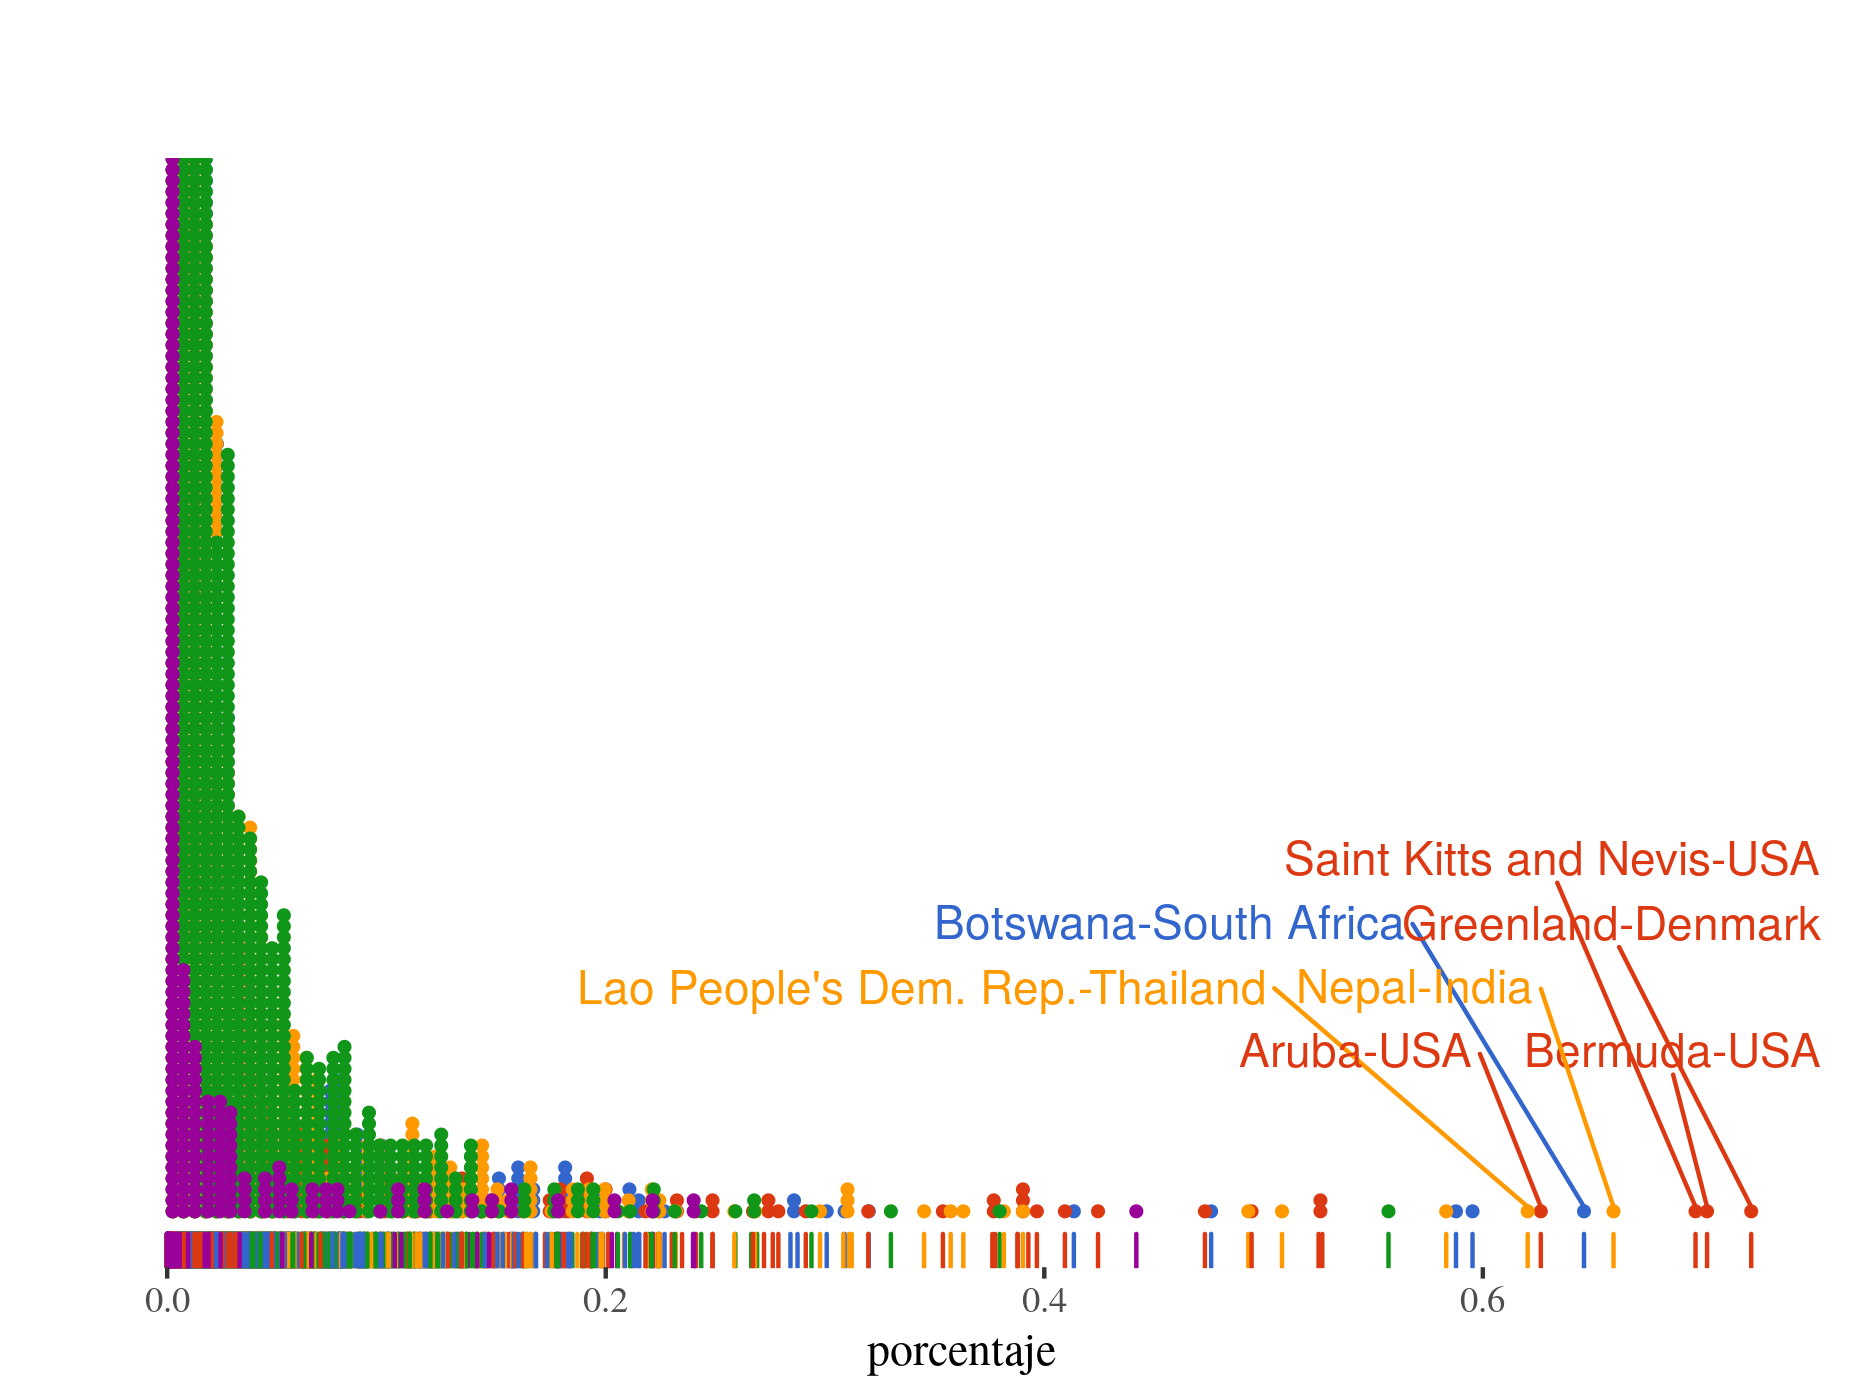
\includegraphics[width=.65\linewidth]{2016_freq_interacciones_3}}
	\subfigure[proporción mayor al 70\%]{\label{fig:rel_dep-2}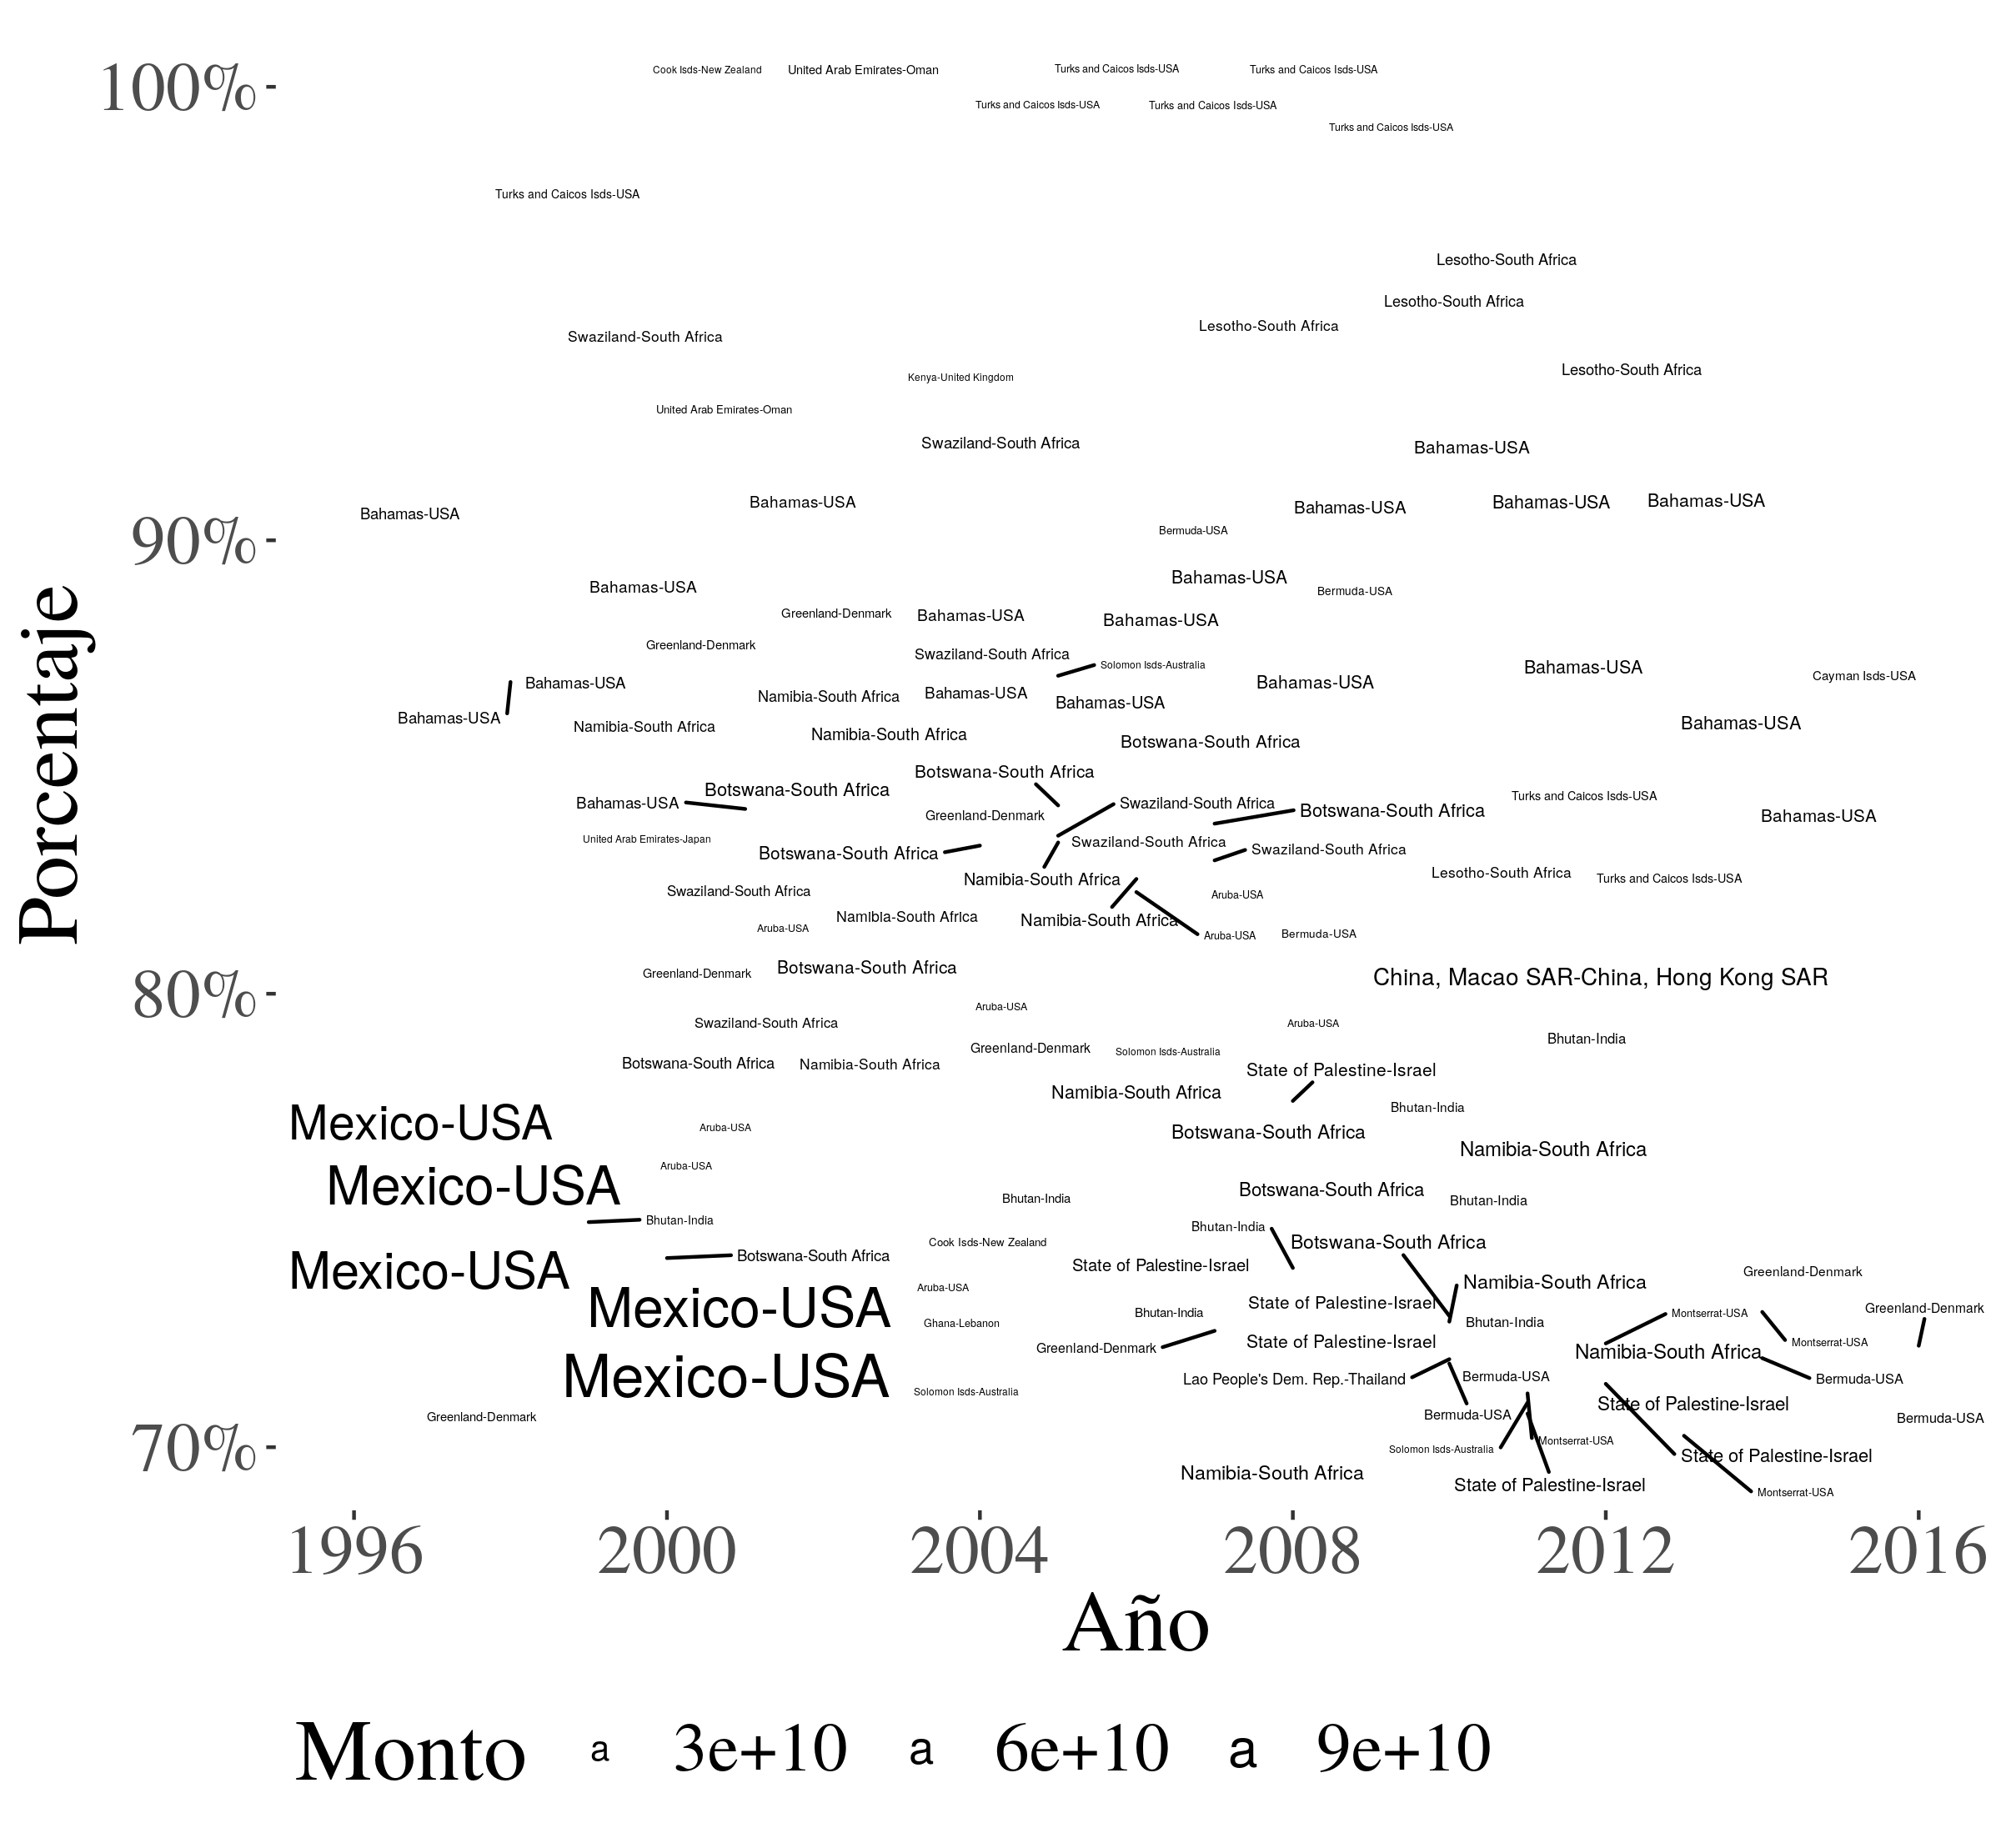
\includegraphics[width=.65\linewidth]{relaciones_dependientes_EDA}}
	\caption{Interacciones Según porcentaje de importaciones que representa al país importador. Destacado par Importador-Exportador.1996-2016}
	\label{fig:rel_dep}
\end{figure}





Por su parte, en la figura \ref{fig:rel_destacadas-1} se puede observar la distribución de los montos comerciados en el año 2016, destacando aquellas relaciones de mayor volumen. Al igual que en la figura \ref{fig:rel_dep-1}, también se observa una fuerte asimetría a derecha, siendo las relaciones más importantes en el continente asiático y Americano. En particular, Las importaciones de Estados Unidos desde México, Canadá y China. También destacan las exportaciones de China, además de la ya mencionada, a Japón y Hong-Kong. Estas relaciones no corresponde caracterizarlas de tipo dependiente en un sentido de intercambio desigual, dado que se trata de volumen, y aquellas que destacan resultan de importancia tanto para exportador como para el importador. Se podría decir que estas son relaciones de alta interdependencia.

En este sentido, la figura \ref{fig:rel_destacadas-2} muestra las cinco relaciones más importantes de cada año. Nuevamente lo que se observa es una repetición en las duplas Importador-Exportador entre año y año. Destaca sobre todo el rol de Estados Unidos como importador de China en primer lugar, y Canadá y México en menor volumen. Es importante observar que las exportaciones de China a Estados Unidos toman una importancia creciente en el tiempo y para el final de la serie se encuentran por fuera de la nube de puntos. 


\begin{figure}
	\centering
	\subfigure[2016]{\label{fig:rel_destacadas-1}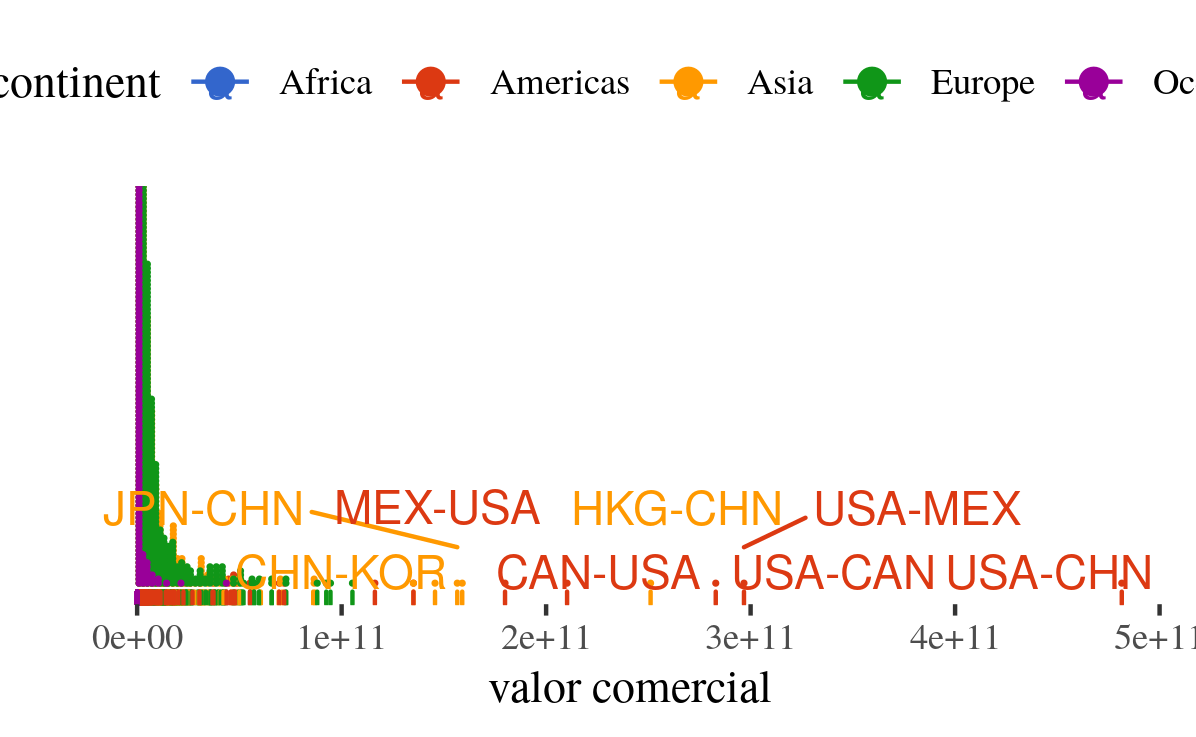
\includegraphics[width=.65\linewidth]{2016_freq_interacciones_0}}
	\subfigure[Top 5 por año]{\label{fig:rel_destacadas-2}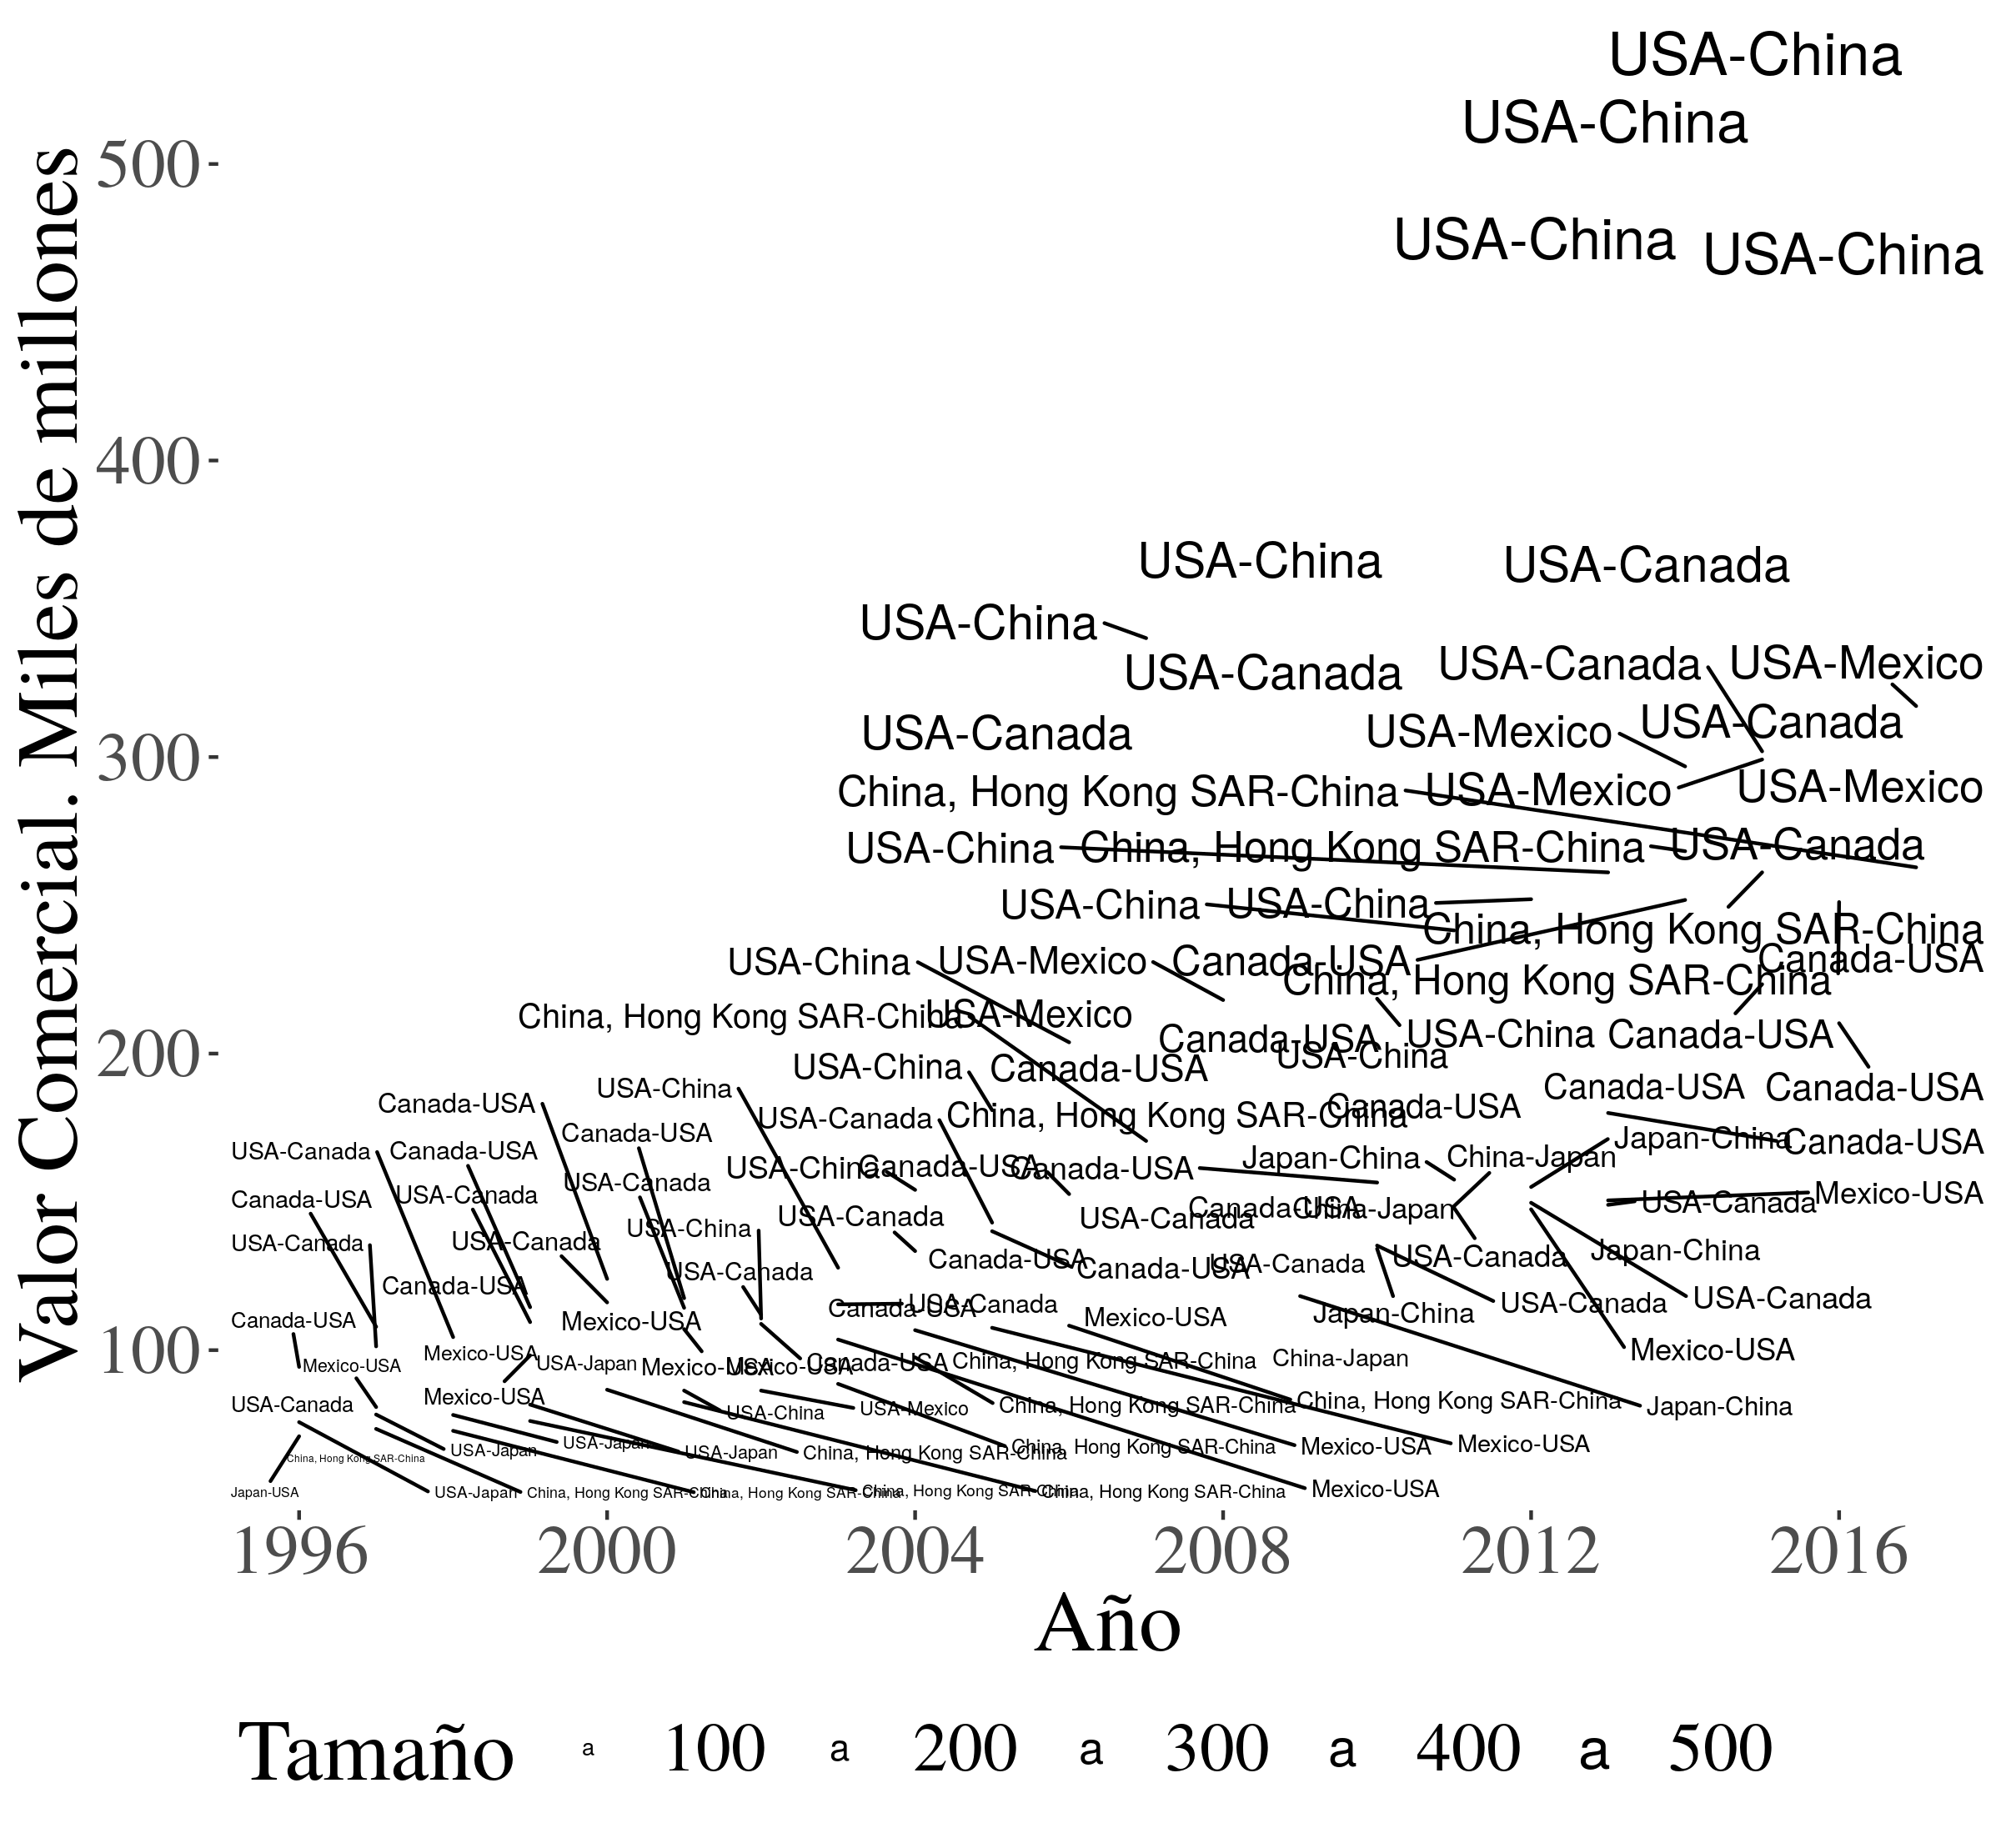
\includegraphics[width=.65\linewidth]{relaciones_destacadas_EDA}}
	\caption{Interacciones. Según valor comercial. Destacado par Importador-Exportador. 1996-2016}
	\label{fig:rel_destacadas}
\end{figure}


Esto también se puede apreciar en relación al total de las relaciones comerciales, en la figura \ref{fig:hexplot} donde se incluye la totalidad de las relaciones comerciales para la serie entre 1996 y 2017. Allí se observa que la absoluta mayoría de las relaciones comerciales constituyen montos menores, y que una proporción menor se realiza por montos de hasta cien mil millones de dólares anuales. También se observa un número creciente de operaciones por montos arriba de los cien mil millones de dólares anuales. Finalmente, también cabe destacar nuevamente la anomalía que representa respecto del resto de los datos las exportaciones desde China a Estados Unidos en la segunda mitad de la serie.  

\begin{figure}
	\centering	
	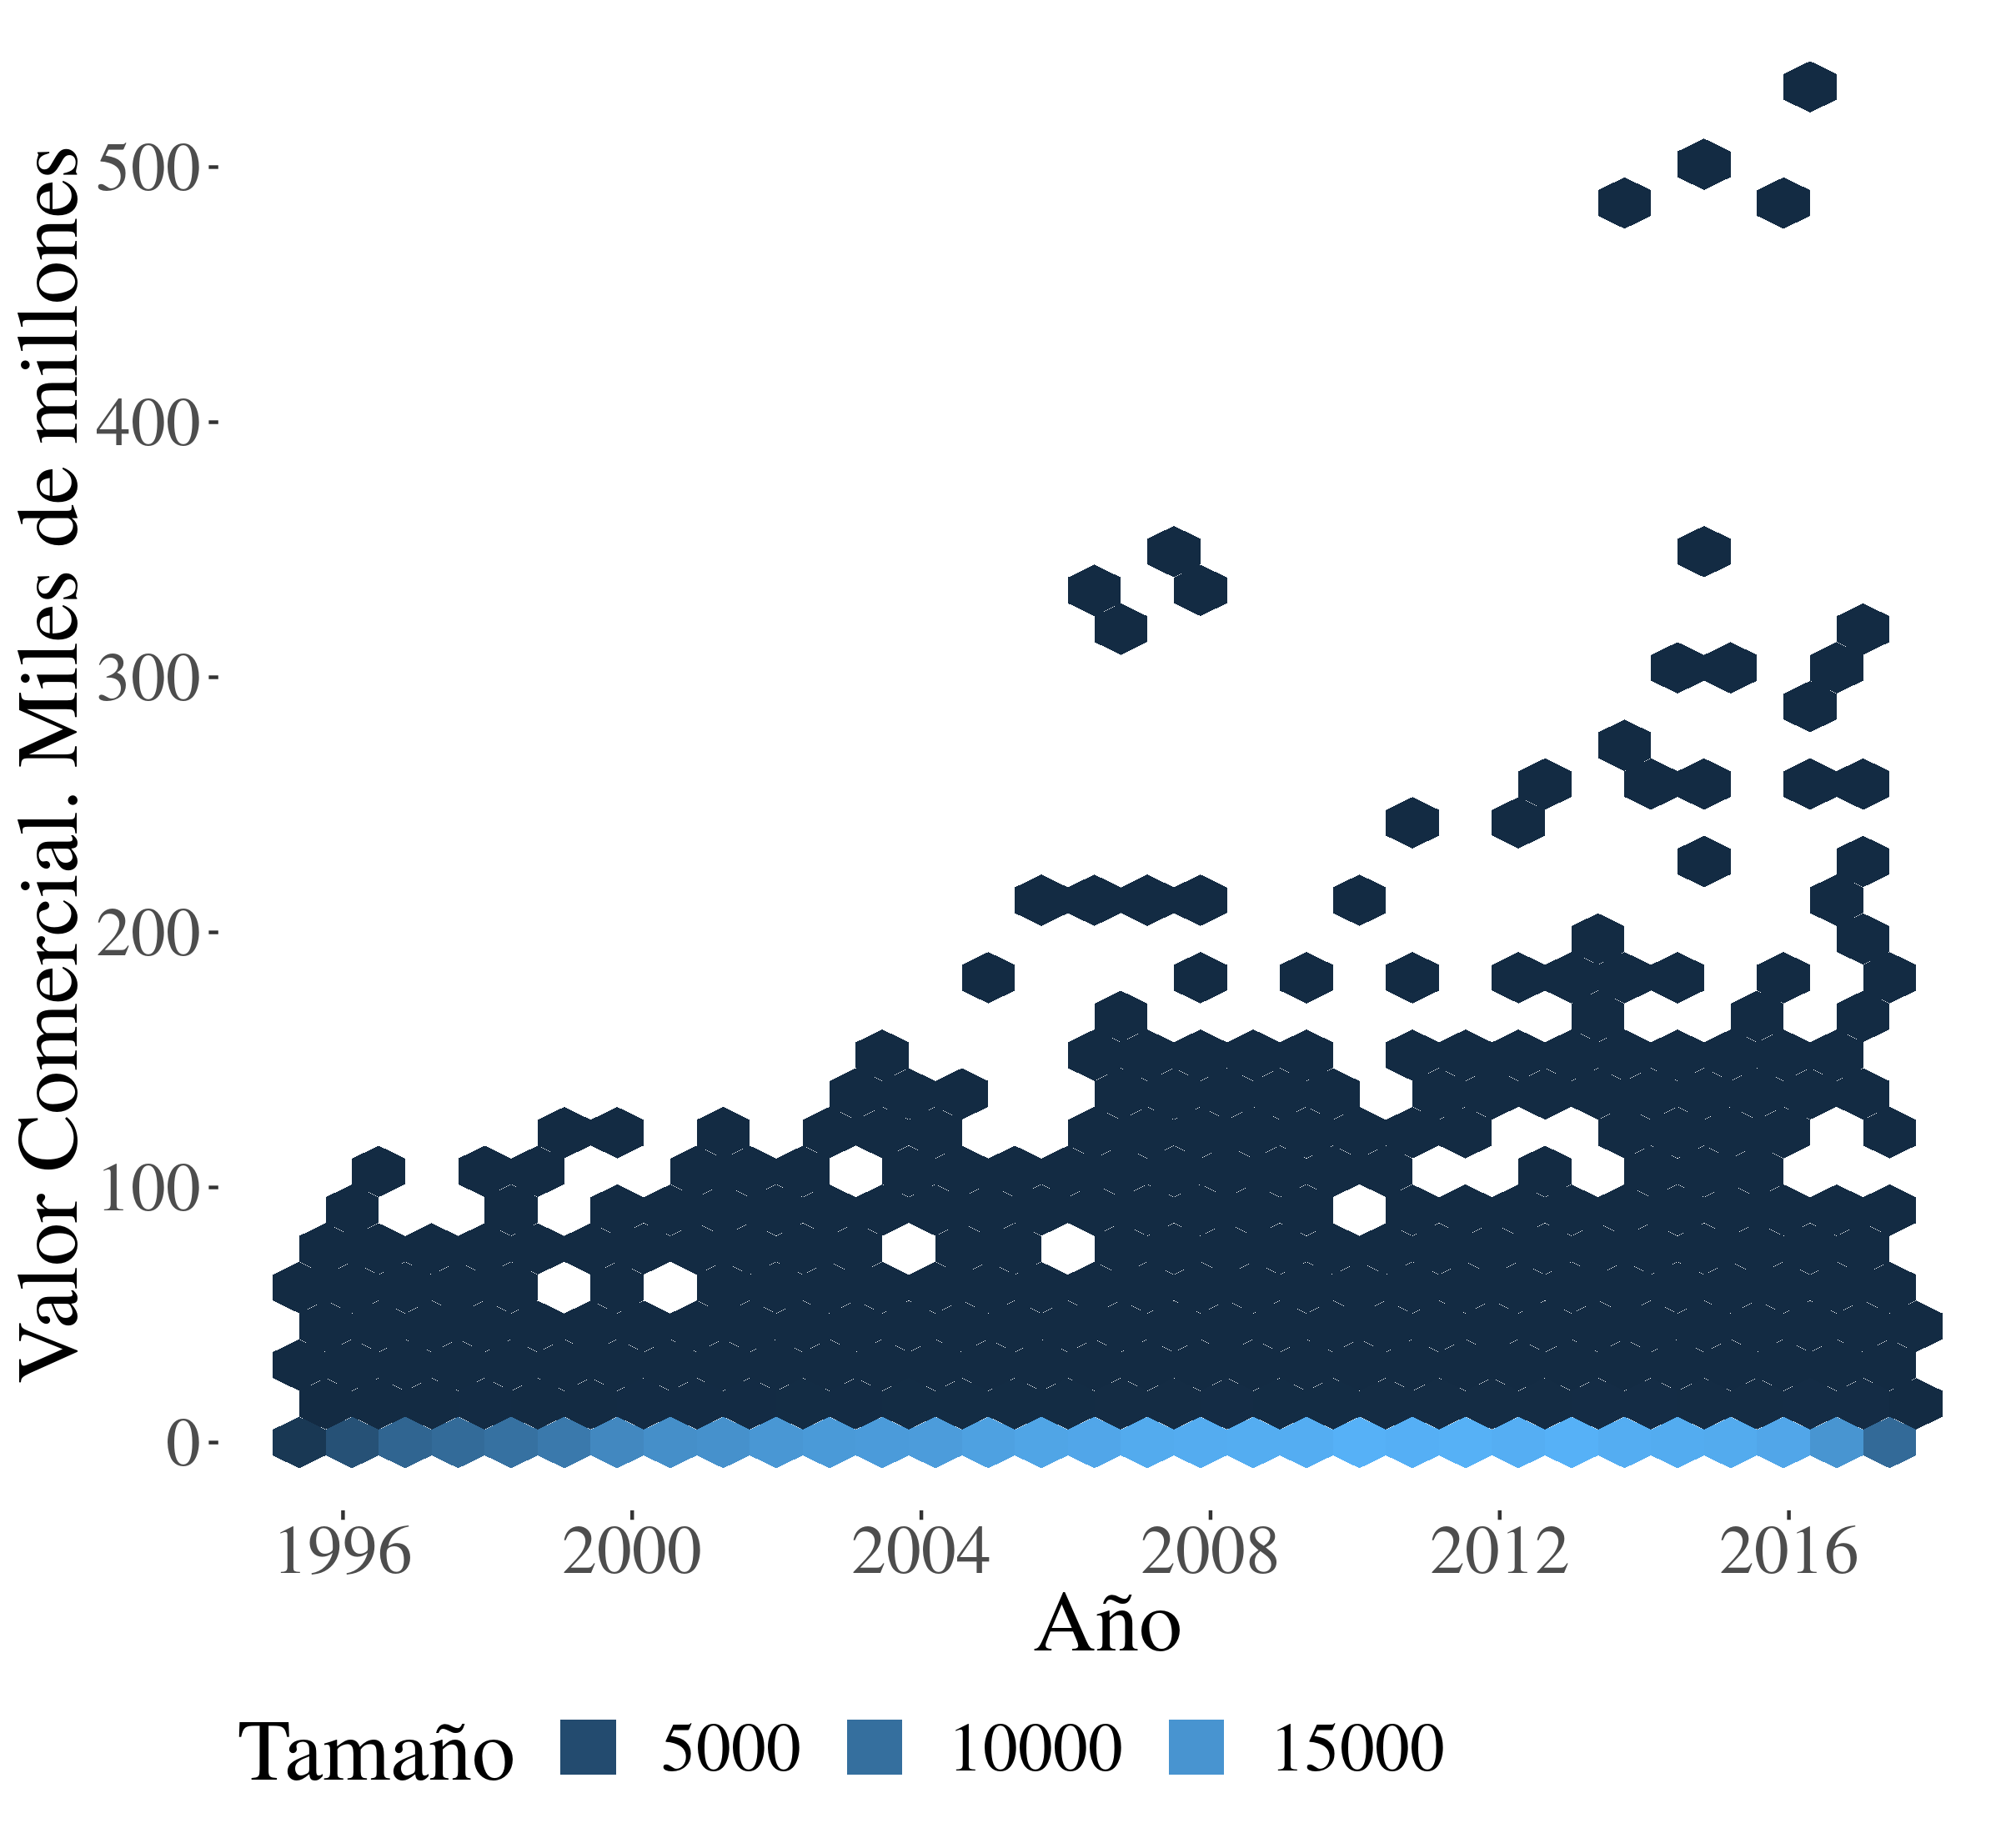
\includegraphics[width=.65\linewidth]{relaciones_96_2016_EDA}
	\caption{Interacciones. Según valor comercial. 1996-2016}
	\label{fig:hexplot}
\end{figure}


\section{Metodología}

\subsection{Fuentes de información}
\info{mover a la introducción. Vale para toda la tesis}

La modelización del comercio internacional como un grafo requiere de los datos del flujo anual de comercio bilateral para el total de las mercancías, para la mayor cantidad posible de países, idealmente todos ellos. Dado que los datos del comercio bilateral son realizados por cada país involucrado, es necesaria una base de datos en la cual se haya recolectado la información provista por cada país, y que a su vez haya sido consolidada frente a las posibles, y de hecho abundantes, contradicciones que se presentan entre los reportes oficiales de los países involucrados. En particular, dado que toda importación para un país es una exportación de otro, y que el registro de los datos se realiza de forma nacional, existe una duplicación formal de la información, que no siempre es coincidente. Por esto, se recurrió a una base previamente consistida por un organismo internacional oficial, la Organización Mundial del Comercio (de aquí en más OMC)\footnote{https://comtrade.un.org/}, y la API que dicho organismo provee para descarga de datos. La información analizada  en las secciones tercera y cuarta, del período 1996-2016, proviene dicho organismo.   


Los datos utilizados para el análisis de largo plazo, entre los años 1948 y 2000 proviene del trabajo realizado por \cite{Gleditsch2002}, que también es utilizado en otros trabajos de modelización del comercio internacional mediante redes complejas \cite{Fagiolo2010}.

\subsection{Construcción del grafo}

Un grafo (o red) se define como un conjunto de nodos y aristas, donde cada nodo representa una entidad, mientras las aristas representan la existencia de una relación entre dos entidades. La representación algebraica del grafo se realiza mediante la denominada matriz de adyacencia, donde las filas representan los nodos de salida, mientras que las columnas representan el nodo de entrada. Por lo tanto, el elemento $a_{ij}$ de dicha matriz representa a la arista que va desde i hacia j.

En el caso de las redes pesadas, una arista, $a_{ij} \in \mathbb{R}$, denota la intensidad de la relación entre los nodos $i$ y $j$. Por su parte, en las redes binarias, $a_{ij} \in \{0,1\}$ define cualitativamente la relación, dónde $a_{ij} = 1$ si existe la relación y $a_{ij} = 0$ sino. Este último tipo de grafos sera el utilizado para el presente trabajo, dado que se cuenta con una mayor cantidad de métricas para caracterizar los grafos de este tipo.      
A su vez, las redes pueden ser tanto dirigidas como no dirigidas. En el primer caso, la relación no tiene un sentido definido, y por lo tanto $a_{ij} = a_{ji}$, mientras que en el segundo caso tal igualdad no es necesaria, y la presencia de una relación tiene un sentido definido. Si bien en la bibliografía existen autores que plantean que la simetría del intercambio comercial es fuerte, y por lo tanto no es necesario utilizar un grafo dirigido para su representación \cite{Fagiolo2007}, en el presente trabajo se sostiene que esto depende fuertemente de la forma de construcción de la red, en particular si se trabaja con un grafo no ponderado, y por lo tanto hay un riqueza interpretativa que se pierde si se utiliza una red no dirigida.       


Sobre una red se puede calcular una serie de medidas de resumen que permiten caracterizarla. Éstas pueden referirse a un atributo propio del grafo, o bien de cada nodo o arista. Si bien las posibles métricas son muchas, en el presente trabajo nos limitamos a aquellas que se definen a continuación. \par    
Dos nodos se dicen conectados si existe un recorrido entre ellos, es decir, una secuencia de aristas y nodos entre estos. De un grafo se dice que esta conectado, si todos sus elementos lo están. \par
El diámetro $d_m$ de una red es la máxima distancia entre cualquier par de nodos. En teoría de grafos se considera la distancia entre un par de nodos como el camino más corto que se puede realizar entre éstos. Es decir, el diámetro de un grafo no pesado se considera como la cantidad de aristas que hay entre los dos elementos más lejanos del grafo, considerando el recorrido más corto entre ambos. 

$$
d_m = max(d_{uv})
$$
donde $d_{uv}$ es la distancia entre los nodos u y v, definida como:
$$
d_{uv} = min(L(P))
$$
con $P = (v_1, v_2, ..., v_n)$,un conjunto de n vértices, donde $v_i$ es adyacente a $v_{i+1}$, y siendo $L(P)$ la longitud del camino P, definida como:
$$
L(P) = \sum_{i=1}^{n} w_i
$$
En el caso de una red no ponderada, $w_i = 1$ y por lo tanto, la longitud de un camino es la cantidad de elementos que lo componen. \par
La densidad $De_m$ de una red es la relación entre la cantidad de aristas de la red y la máxima cantidad de aristas potenciales de la misma. 

$$
De_m = \frac{|A|}{|V|(|V|-1)}
$$

Siendo $|A|$ el número de aristas y $|V|$ el número de vértices, o nodos, del grafo. $De_m \in [0,1]$. Aquellas redes con una densidad cercana a 0 se las considera dispersas, mientras que aquellas con una densidad cercana a 1 se las considera grafos densos. \par

A su vez, existe una serie de medidas de centralidad de nodos que caracterizan la importancia de los mismos en la red. Las utilizadas en el presente trabajo son la intermediación, cercanía y autovalor. \par
La centralidad de intermediación mide el rol de un nodo $i$, $C_{BET}(i)$, como puente entre los demás nodos, considerando sus caminos más cortos. Se define como:
$$
C_{BET}(i) = \sum_{j,k \neq i} \frac{b_{jik}}{b_{jk}}
$$
donde $b_{jk}$ son todos los caminos más cortos entre los nodos $j$ y $k$, y $b_{ijk}$ son los caminos más cortos entre $j$ y $k$, que pasan por $i$. \par
La centralidad de cercanía es la distancia promedio que tiene un nodo con los demás nodos con los que esta conectado. Formalmente: 
$$
C_{cer}(i) = \frac{1}{\displaystyle \sum_{j \neq i} d_{i,j} }
$$

La centralidad de grado se define como la cantidad de aristas de un nodo. En el caso de los grafos dirigidos, se puede considerar un grado de entrada, así como un grado de salida, si las aristas van en dirección al grafo o desde el grafo, respectivamente.
La centralidad de autovalor, por su parte, caracteriza la importancia de un nodo considerando la de sus nodos vecinos. Si asumimos linealidad:

$$
x_i'= \sum_{j=1}^{N} a_{ij}x_{j}
$$
$$
x' = Ax
$$
Siendo A la matriz de adyacencia de la red. si $x'$ es el vector de centralidades de la red, entonces podemos plantear $Ax^* = \lambda x^*$ donde $x^*$ es la solución y  $\lambda$ es el autovalor asociado al mayor autovector.  Por lo tanto, podemos definir la medida de centralidad de autovalor como

$$
x_i^*=\frac{1}{\lambda}  \sum_{i} A_{ij}x_{j}^*
$$

Esta medida tiene la propiedad de considerar la importancia de un nodo a partir de la importancia de aquellos nodos con los que esta conectado, y con los que éstos están conectados, etc. En el presente trabajo también se considera a la centralidad de autovalor ponderado como una alternativa, donde el peso esta definido por el volumen de dinero comerciado entre los países. Para calcularlo, se multiplica la matriz de adyacencia por una matriz de pesos. Por lo tanto

$$
x_i^{pond}=\frac{1}{\lambda}  \sum_{i} WA_{ij}x_{j}^{pond}
$$

Estas medidas de centralidad pueden ser resumidas para el grafo en su conjunto mediante una agregación de algún tipo, como el promedio, máximos y mínimos, etc. En el presente trabajo se utilizan de ambas maneras, tanto para definir la importancia de un país en particular en el grafo, como para caracterizar a la red en su conjunto.
\par

El Coeficiente de clustering estima la cohesividad local, midiendo la probabilidad de que dos nodos que comparten un vecino estén conectados. Para calcularlo, se mide en primer lugar el grado de agrupamiento de cada nodo, tomando la vecindad del mismo, es decir, todos aquellos nodos con los que esta conectado, y se calcula el cociente entre las aristas existentes y la máxima cantidad de aristas posibles:

$$
C_i = \frac{|A_i|}{|V_i|(|V_i|-1)}
$$
siendo $|A_i|$ las aristas en el subgrafo de la vecindad de i, y $|V_i|$ los vértices del subgrafo de la vecindad de $i$. Nótese que esta medida no representa lo mismo que la densidad, si bien las ecuaciones sean similares, dado que en el clustering se analiza solamente la vecindad de un nodo, mientras que la densidad se refiere a toda la red.
Si quisiéramos caracterizar a toda la red según el coeficiente de clustering, podemos calcular el promedio del mismo para todos los nodos, también conocido como transitividad del grafo, que se define como el promedio del grado de agrupamiento de los nodos. Es decir:

$$
\Bar{C} = \frac{1}{n} \sum_{i} C_{i}
$$ 


Por último, también se considera la correlación de grado entre las aristas. Esta se calcula como la correlación de Pearson entre el grado de nodos adyacentes. Si la correlación es fuerte y positiva, esto implica que la red es de tipo selectiva, lo que indica que los nodos de mayor grado tienden a conectarse con otros nodos de mayor grado. Si la correlación es negativa y fuerte, esto indica que la red es no selectiva o heterogénea, lo que implica que los nodos más importantes de la red tienden a conectarse con nodos poco centrales. 


\subsection{Software utilizado}

Para el presente trabajo se utilizó el lenguaje de programación estadística \texttt{\textbf{R}}\citep{RCoreTeam2017}, junto con sendas extensiones del mismo. Aquellas que resulta importante mencionar son \texttt{igraph}\citep{Csardi2006} para la construcción de los grafos y las medidas de resumen de los mismos; \texttt{tidyverse}\citep{Wickham2017} para la manipulación de la información y elaboración de los gráficos. Para esto último, también se hizo uso de  \citep{Wilke2017,Arnold2017,Neuwirth2014,Slowikowski2017,Vu2011}, como complementos de \texttt{ggplot}. Por su parte, los códigos de los países provienen de \citep{Arel-Bundock2017}.

\subsection{El comercio internacional como una red compleja}

La modelización del comercio internacional como un grafo conlleva una serie de simplificaciones de la información original. Nos encontramos en primer lugar que toda compra es a su vez una venta, y que por lo tanto la información se puede interpretar de ambas maneras. Por su parte, dado que lo que se busca representar es existencia de un vínculo comercial entre dos países, considerar toda compra o toda venta como la existencia de éste vínculo resultaría exagerado. Por lo tanto, es necesario establecer un punto de corte a partir del cual se considere que existe una relación comercial entre la dupla de países en cuestión. Sin embargo, tal punto de corte no se debe considerar en término absolutos, como el monto comerciado, ya que dicho monto esta sumamente determinado por el tamaño de los países en cuestión. En otros términos, una determinada masa de dinero es significativa para un país en función del valor total comerciado por el mismo. Por lo tanto, es necesario considerar el umbral en términos relativos respecto al tamaño de los mismos.

En este punto se abre una serie de consideraciones respecto al denominador a utilizar. Si se normaliza por el tamaño de la economía, el Producto Bruto Interno (PBI), se está considerando no sólo la importancia relativa de ese vínculo comercial respecto del total comerciado, sino también el grado de apertura de dicha economía. En ese sentido, si se quisiera analizar el rol de un país en el comercio internacional, independientemente del tamaño real de su economía, lo más correcto es normalizar por el volumen total comerciado, y no por su PBI. De esta forma, se puede considerar un punto de corte como un tanto por ciento de las importaciones o exportaciones del país que reporta la transacción.

Dado que se considera que la información de las importaciones suele ser más confiable que la de las exportaciones \citep{Fan2014}, en el presente trabajo se utiliza en la generalidad de los casos el punto de corte como un porcentaje del total de las importaciones del país importador. No obstante, dada la construcción de dicho punto de corte, la interpretación de los resultados varía. Si se utiliza la información provista por el importador, la dirección de la arista resultante es desde el importador hacia el exportador, el sentido contrario al de las mercancías, es decir, el sentido del dinero. Esta arista sólo existe sí resulta significativa para el país importador.     

Podemos entonces, utilizar un grafo binario dirigido. Dados N países, definimos la matriz de adyacencia NxN, dónde:

$$
a_{ij} = 
 \begin{cases} 
      1 & si \frac{x_{ij}}{x_{i\cdot}}\geq u \\
      0 & sino 
  \end{cases}
$$

Donde $u$ representa el umbral elegido, y $x$ representa el volumen comerciado.   
Para el caso de las importaciones, $x_{ij}$ representa el monto total comerciado desde el país $j$ hacia el país $i$, mientras que $x_{i\cdot}$ representa el total de las importaciones del país $i$. En el grafo de exportaciones, al contrario, $x_{ij}$ representa el monto total comerciado desde el país $i$ hacia el país $j$, mientras que $x_{i\cdot}$ representa el total exportado por el país $i$.          

Dado que la restricción se construye por la importancia relativa para el nodo de origen, en general sólo existirá una pequeña cantidad de aristas que salgan de cada nodo, aunque no están limitadas las aristas en dirección hacia el nodo. Más precisamente, la máxima cantidad posible de aristas de salida es igual a $\frac{1}{u}$. Esta cantidad se obtiene sólo cuando el país comercia de forma uniforme con exactamente $\frac{1}{u}$ países. Como se verá más adelante, la distribución del comercio dista mucho de ser uniforme, por lo cual la cantidad de aristas de salida de un nodo se verá fuertemente limitada. Sin embargo, las aristas de entrada al nodo sólo se limita formalmente por la cantidad de nodos en el grafo. 

Por lo tanto, para el grafo de importaciones, cuando se consideren medidas de centralidad de los nodos, se deberá considerar en particular las aristas que están dirigidas en dirección al nodo, y éstas marcaran la importancia de tal nodo como un país productor del mercado mundial, ya que lo que se esta midiendo es si los productos que exporta dicho país resultan significativos o no considerados en las importaciones de los demás países. Por su parte, si se consideran los datos provistos por los países exportadores, las medidas de centralidad de los nodos, estarán reflejando la importancia de tal país como consumidor global, ya que su consumo resulta significativo como exportación para los países que le venden dichas mercancías. 
Dado que, por la forma de construcción de los grafos, resulta distinta la interpretación de la información de las exportaciones y las importaciones, se considerarán alternativamente ambas redes según qué resulte más interesante. 


\subsection{Determinación del punto de corte}

El punto de corte a utilizar, dada la metodología propuesta para discretizar la información del volumen comerciado, opera fuertemente sobre el grafo resultante. La figura \ref{fig:grafo_2016} muestra el grafo según si se utiliza un punto de corte de 1\%, 5\%, 10\%, 15\%, 20\% o 25\%.

\begin{figure}
	\centering
	\subfigure[1\%]{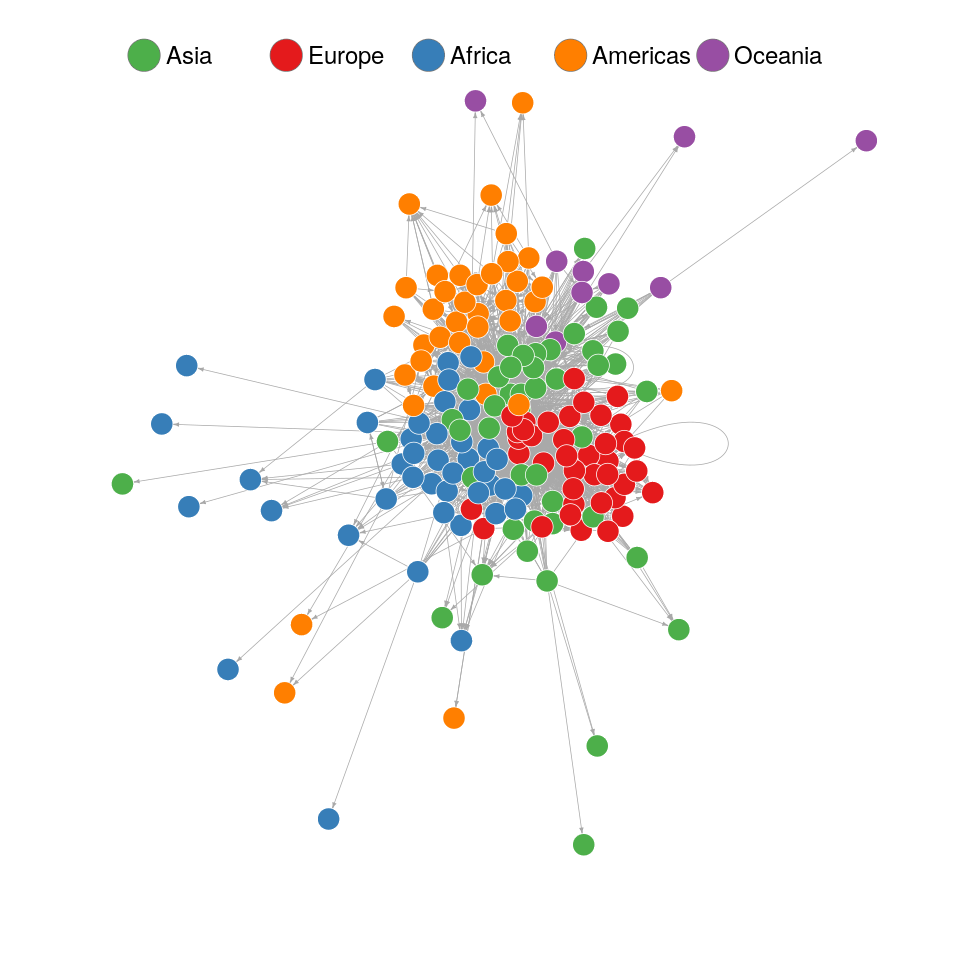
\includegraphics[width=0.45\linewidth]{grafo_2016_1_pcnt}}
	\subfigure[5\%]{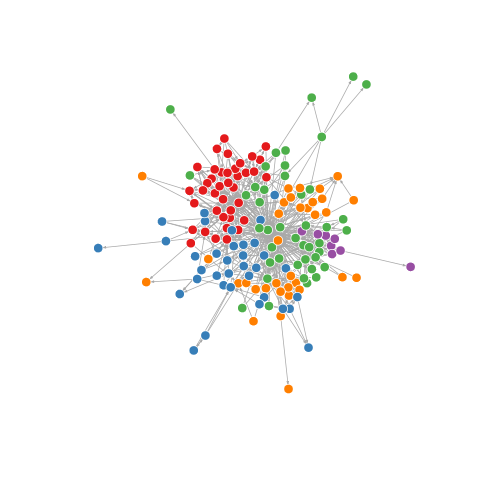
\includegraphics[width=0.45\linewidth]{grafo_2016_5_pcnt}}
	\subfigure[10\%]{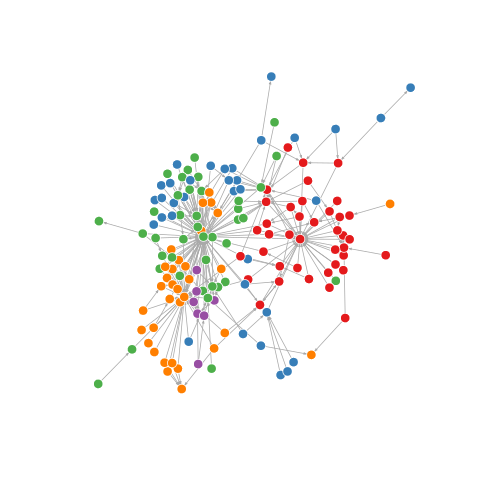
\includegraphics[width=0.45\linewidth]{grafo_2016_10_pcnt}}
	\subfigure[15\%]{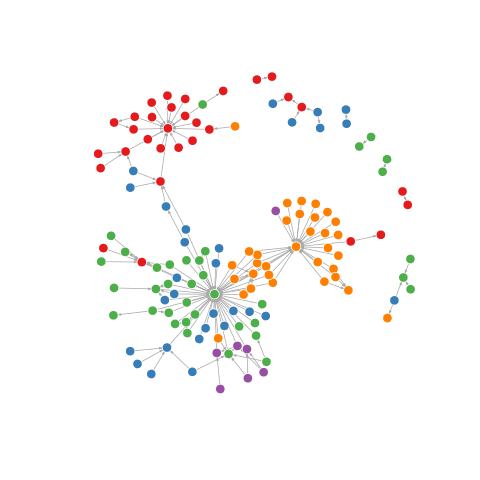
\includegraphics[width=0.45\linewidth]{grafo_2016_15_pcnt}}
	\subfigure[20\%]{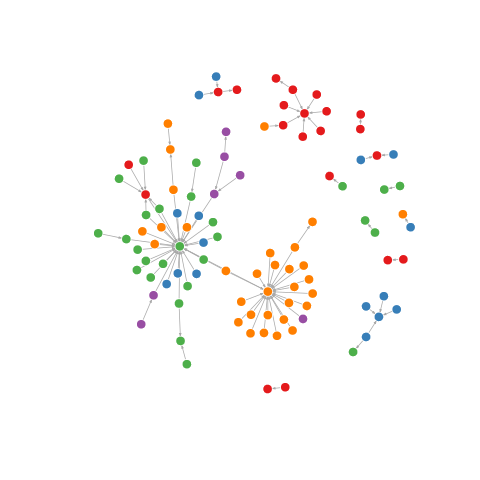
\includegraphics[width=0.45\linewidth]{grafo_2016_20_pcnt}}
	\subfigure[25\%]{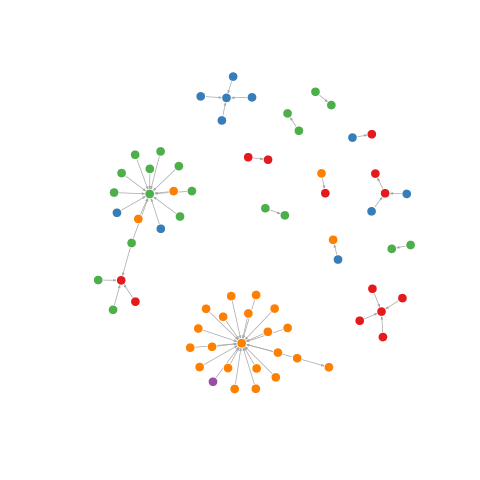
\includegraphics[width=0.45\linewidth]{grafo_2016_25_pcnt}}
	\caption{\textbf{Grafos. 2016, según punto de corte}}
	\label{fig:grafo_2016}
\end{figure}

Se puede observar como hasta un punto de corte del 10\% la red se mantiene unida, aunque disminuye la cantidad de nodos. A partir de este punto, la red deja de estar débilmente conectada y, a la vez que sigue disminuyendo la cantidad de nodos, se observa mejor la importancia de ciertos nodos de alto grado. En particular, uno del continente americano (Estados Unidos) y otro del continente africano (Sudáfrica).


De esto se desprende la importancia de este parámetro en los resultados del modelo. Dado que no se trata de un modelo supervisado, no es posible optimizar el parámetro según alguna medida de bondad de ajuste del modelo. Por el contrario, debemos elegir el punto de corte que resulte más conveniente para los fines del análisis. 

En el sentido de esto último, contamos con varias métricas que permiten caracterizar las propiedades del grafo, así como conocimiento previo respecto a propiedades conocidas y ampliamente aceptadas del comercio internacional. De esta forma, para determinar el punto de corte se propone como metodología utilizar una medida de centralidad que describe un atributo previamente conocido del comercio mundial, y buscar aquél punto de corte en que dicho atributo se expresa más plenamente. Una característica ampliamente estudiada del comercio internacional es su regionalismo \citep{das2004regionalism}, es decir, la tendencia de los países de comerciar en mayor medida con sus vecinos \citep{Head2014}. Si bien no contamos en este trabajo con información respecto de la distancia entre países, de esta característica emerge un fenómeno medible: el nivel de clustering de la red. En este sentido un valor alto en el clustering resulta deseable desde el punto de vista del objeto de estudio. En la figura \ref{fig:centralidad_2016-1} se observa el coeficiente de clustering para la red según el punto de corte utilizado, para cada año de la serie entre 1996 y 2016. Allí se observa que dicha métrica tiene una relación negativa no lineal con el punto de corte. Por lo tanto utilizar un punto de corte bajo resulta conveniente para captar el fenómeno. Sin embargo el máximo se encuentra en el punto de corte igual a cero, esto quiere decir que el regionalismo se expresa más cuando consideramos todos los intercambios, independientemente del monto comerciado. Como se observa en la figura \ref{fig:centralidad_2016-2}, la cantidad de aristas del grafo es significativamente más alta para este punto de corte, y por lo tanto el grafo es sustancialmente más grande y denso, tal como se observa en la figura \ref{fig:centralidad_2016-2}. En este sentido, si bien en la sección siguiente se continúa estudiando diferentes puntos de corte para ver el efecto que esto produce sobre el grafo y sus posibles interpretaciones, se decidió elegir un punto de corte por defecto de 1\% para el resto del trabajo, dado que en dicho valor existe un punto de inflexión en la densidad y número de aristas, lo cual permite resaltar aquellas relaciones comerciales más significativas, a la vez que se maximiza el coeficiente de clustering.

\begin{figure}
\centering
\subfigure[Clustering]{\label{fig:centralidad_2016-1}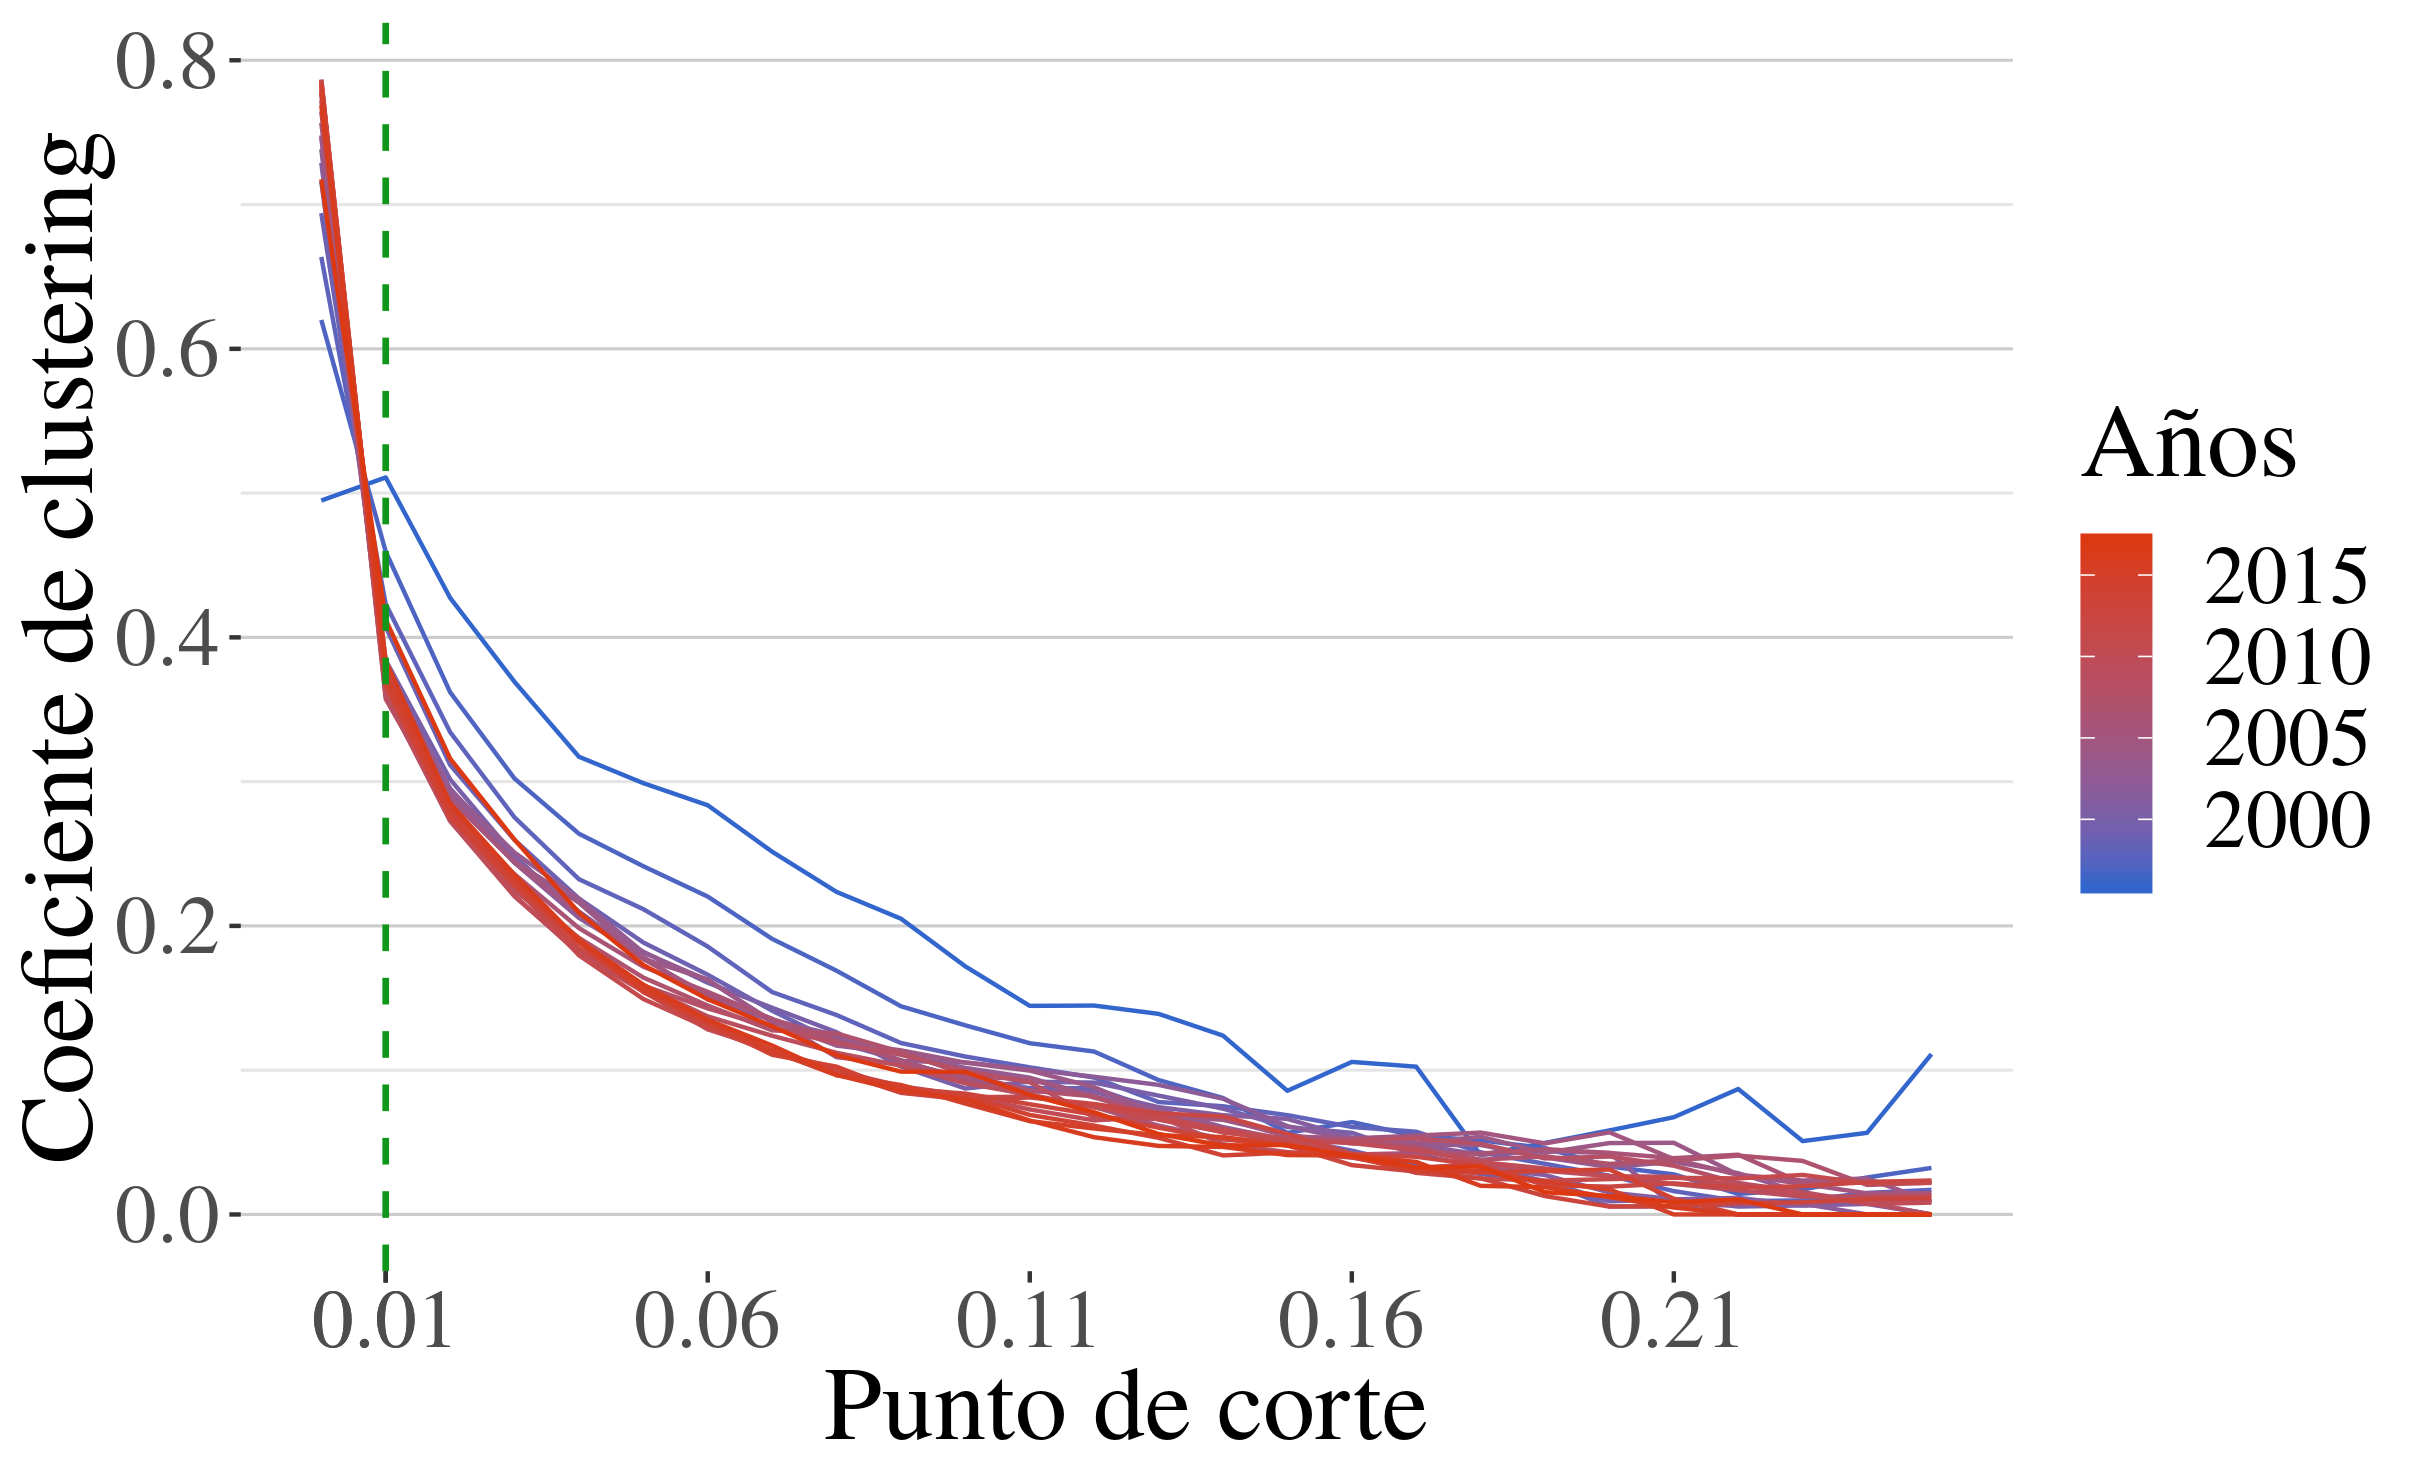
\includegraphics[width=0.45\linewidth]{threshold_x_clustering_x_yr}}
\subfigure[Cantidad de aristas]{\label{fig:centralidad_2016-2}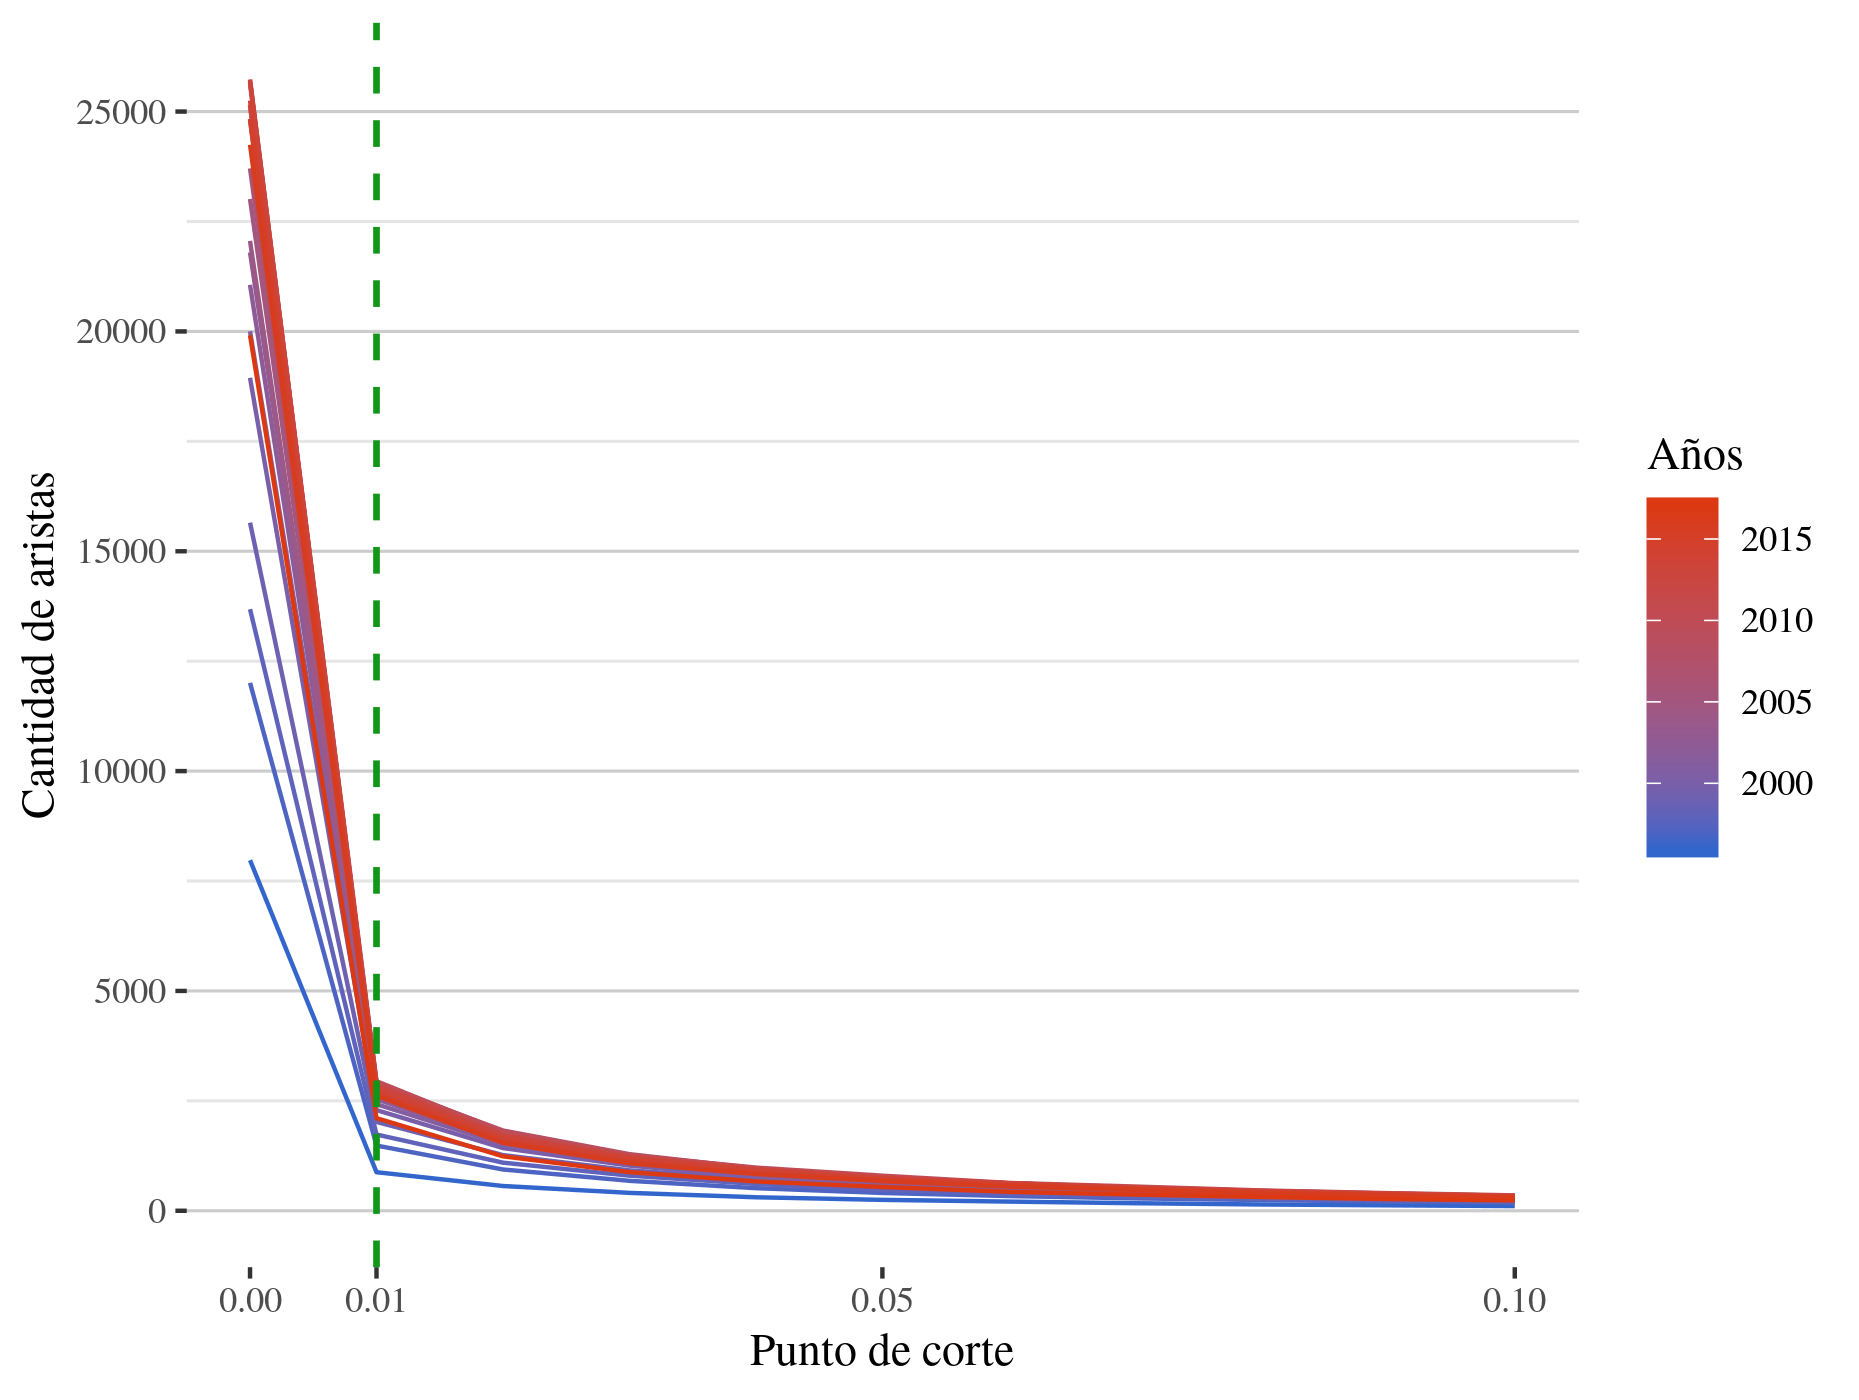
\includegraphics[width=0.45\linewidth]{threshold_x_naristas_x_yr.png}}
\subfigure[Densidad]{\label{fig:centralidad_2016-3}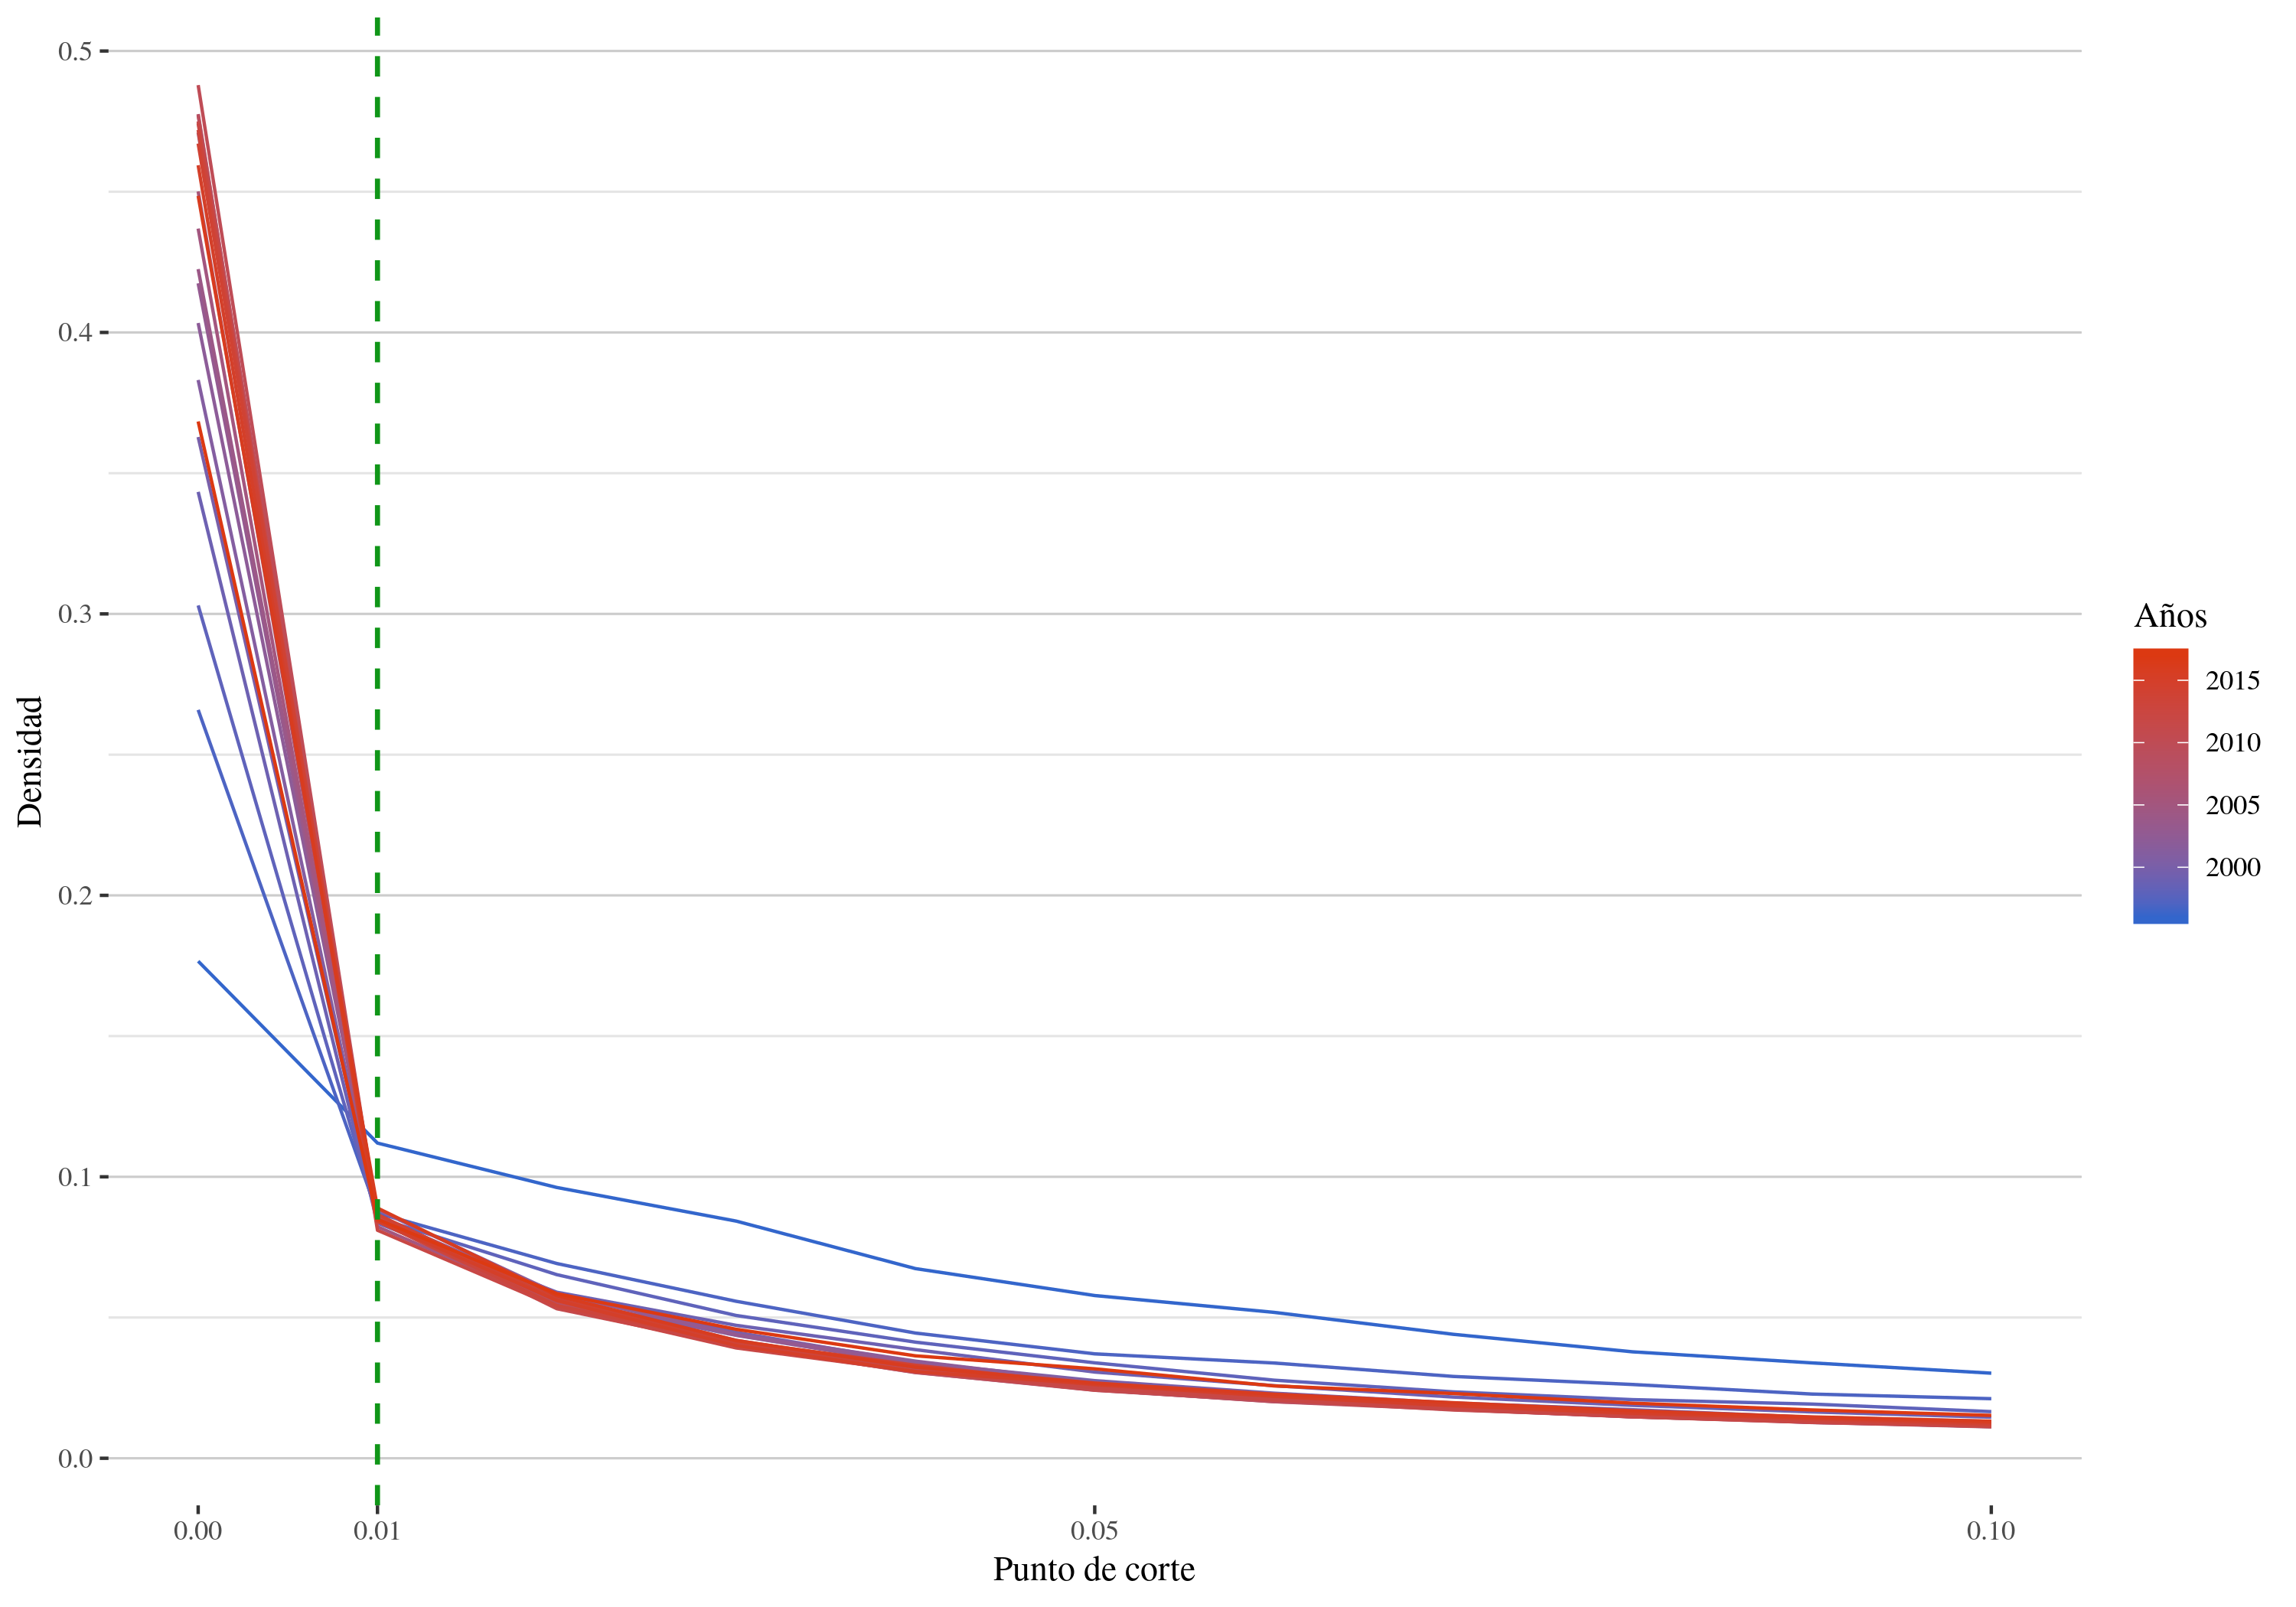
\includegraphics[width=0.45\linewidth]{threshold_x_densidad_x_yr.png}}

\caption{\textbf{Medidas de centralidad}. Importaciones, 2016}
\label{fig:centralidad_2016}
\end{figure}




\section{Resultados}


\subsection{Correlación entre la representación de las exportaciones y las importaciones}

Dada la potencial diferencia en el análisis si se tiene en cuenta las exportaciones y las importaciones, se incorporó esta disyuntiva como una nueva dimensión de estudio. Para ello, se analizó el grado total de cada nodo, para sucesivos puntos de corte, tanto para el grafo que surge de considerar las exportaciones, como para el grafo de las importaciones. En la figura \ref{fig:corr} se pueden observar los resultados. Vale mencionar que sólo se grafican los nodos de mayor grado, aunque se haya considerado al conjunto de nodos para el calculo de la tendencia lineal por continente y el coeficiente de correlación de Pearson.


\begin{figure}
\centering
\subfigure[1\%. Coeficiente de Pearson = 0.96]{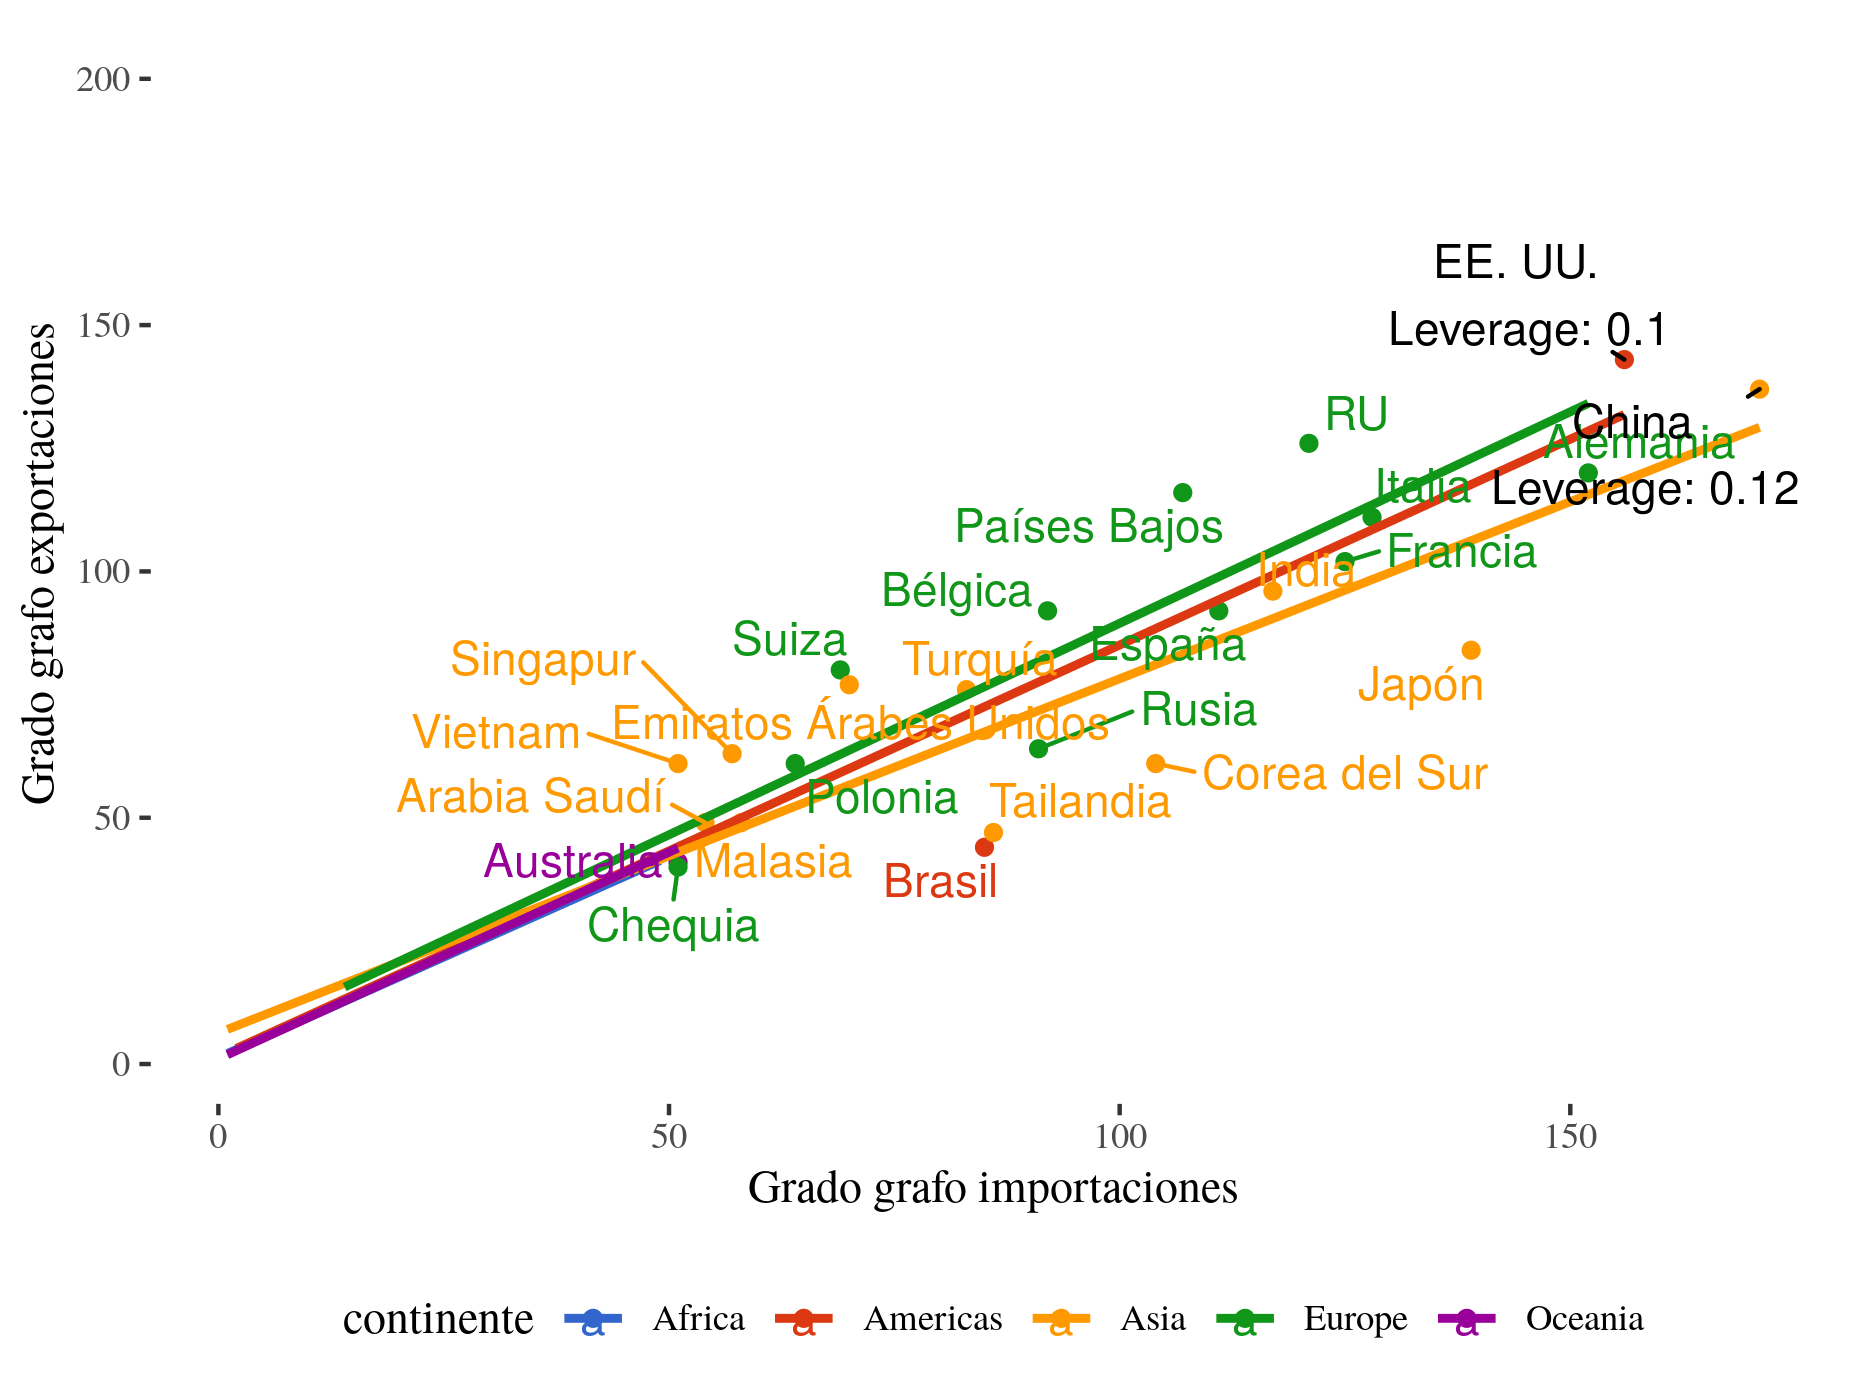
\includegraphics[width=0.9\linewidth]{corr_grados_2016_1_pcnt}}
\subfigure[10\%. Coeficiente de Pearson = 0.77]{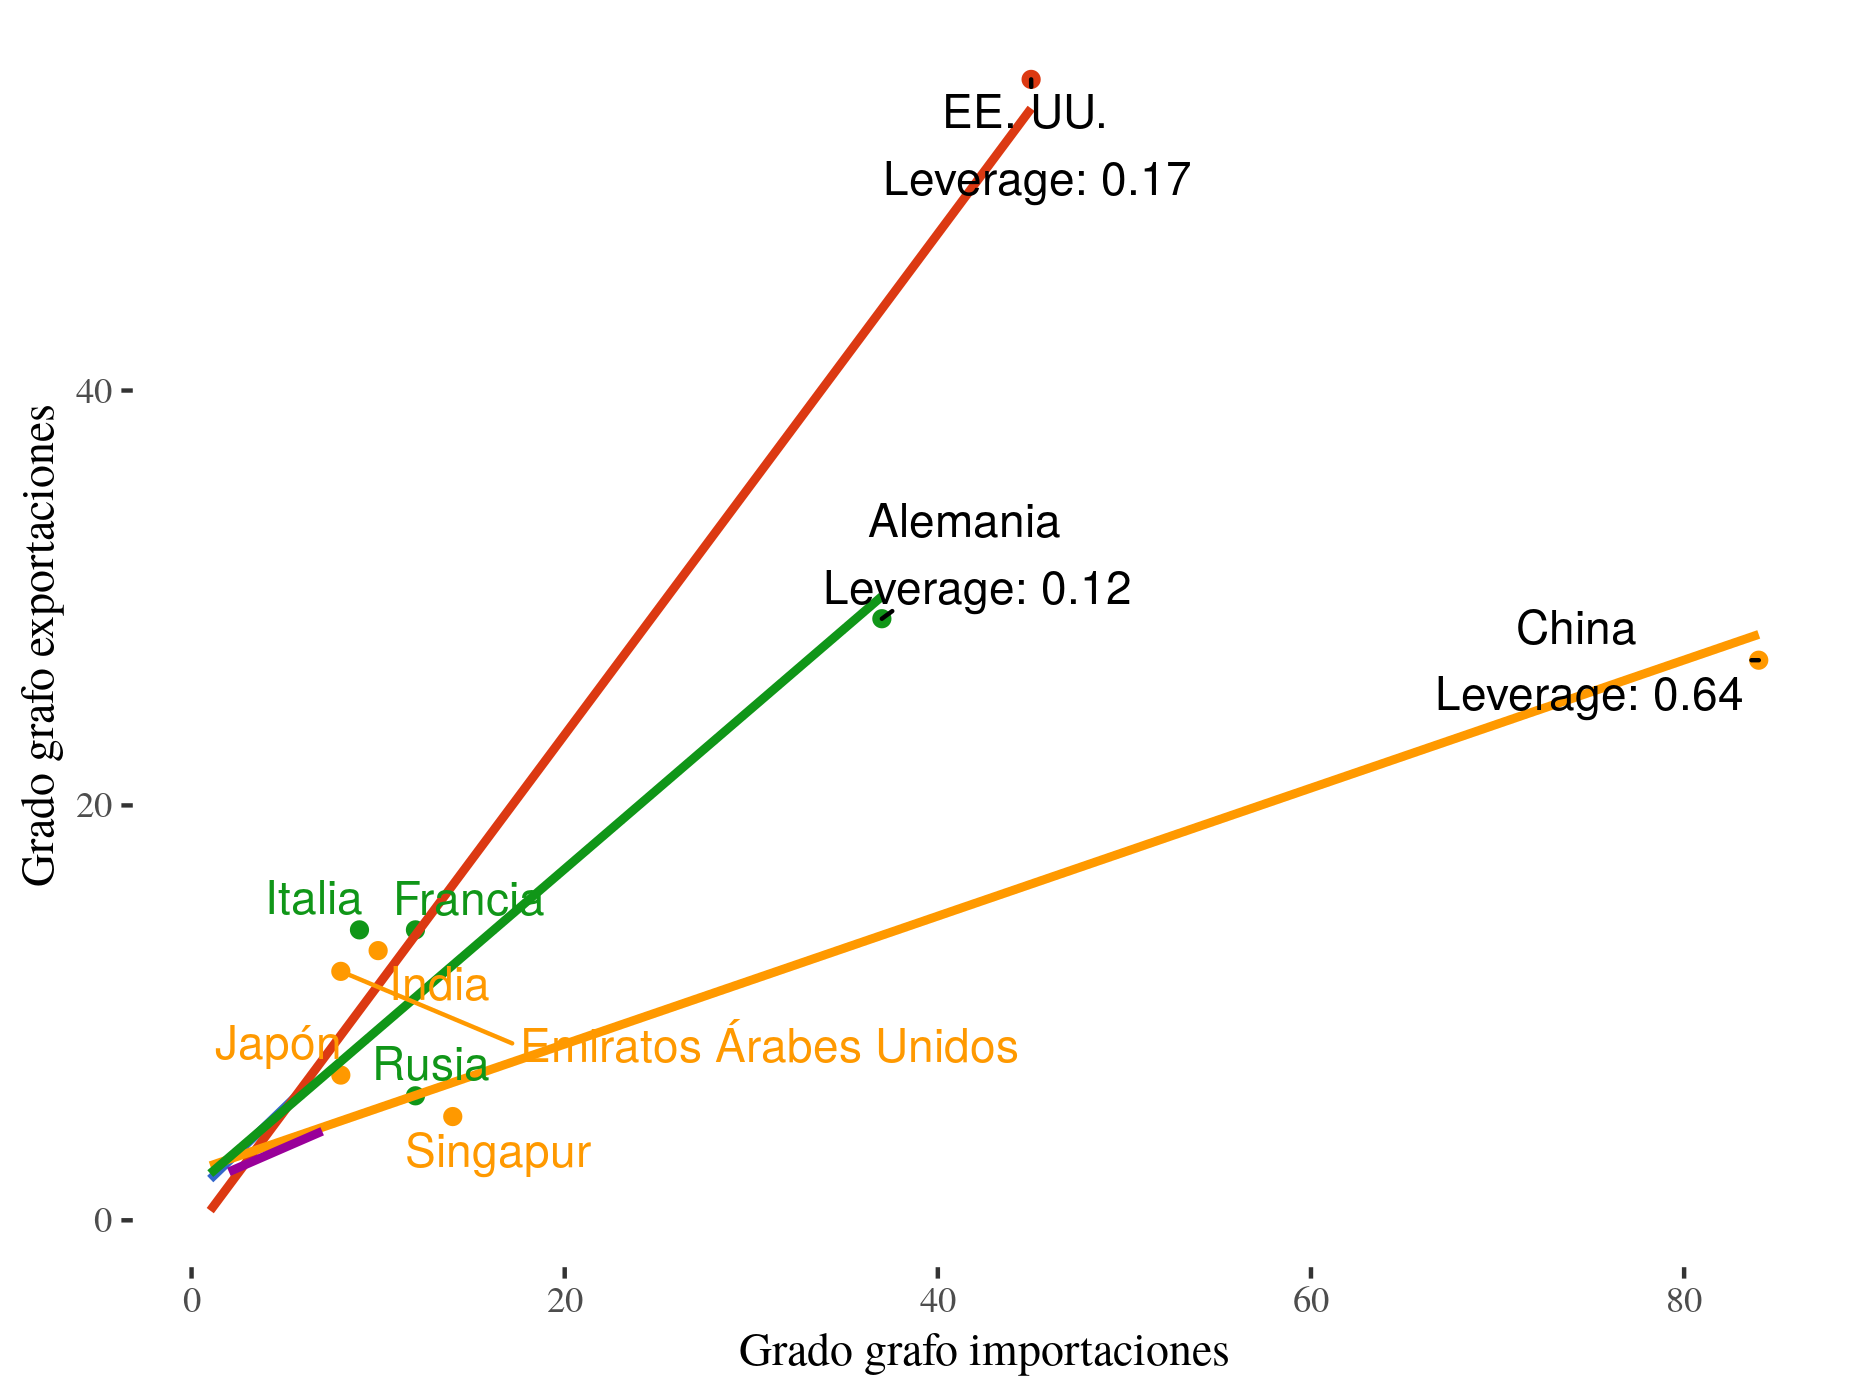
\includegraphics[width=0.45\linewidth]{corr_grados_2016_10_pcnt}}
\subfigure[20\%. Coeficiente de Pearson = 0.81]{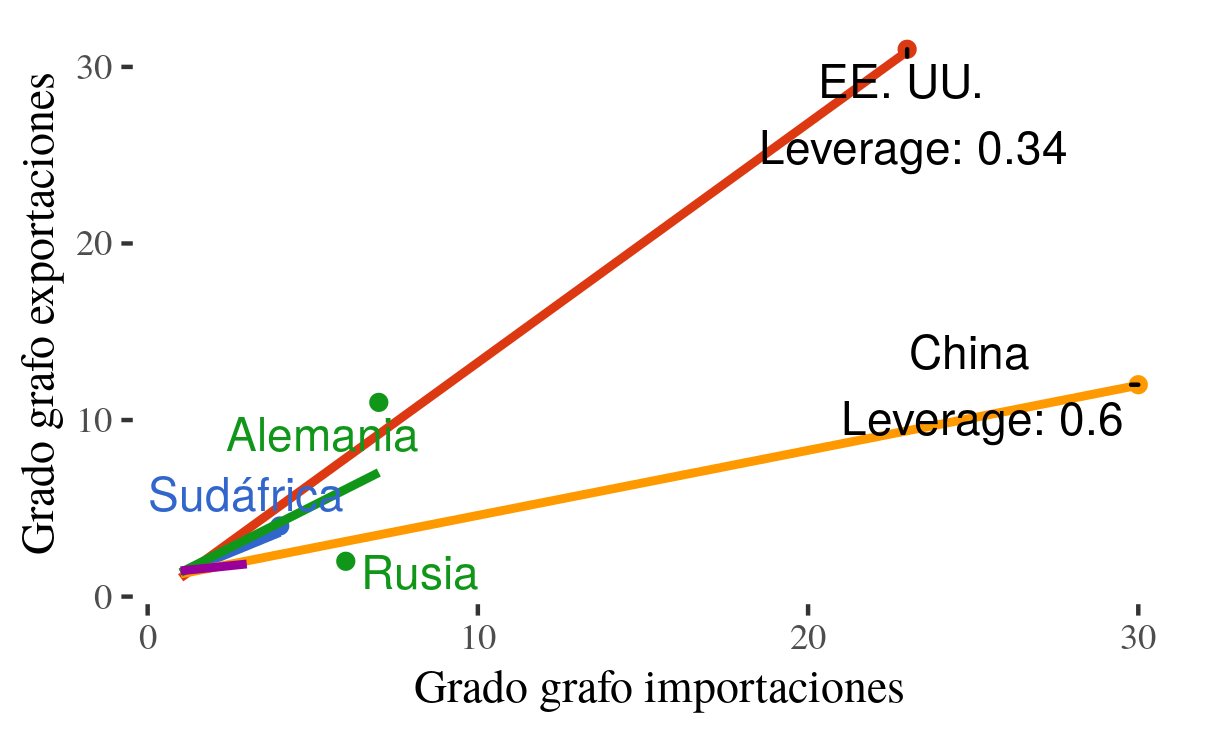
\includegraphics[width=0.45\linewidth]{corr_grados_2016_20_pcnt}}
\caption{\textbf{Grado total.} Multigrafo exportaciones e importaciones. Año 2016}
\label{fig:corr}
\end{figure}


La correlación entre los grafos resultantes oscila entre el 0.72 y 0.96 si se consideran puntos de corte de entre el 1\% y el 25\%, por lo que se puede considerar que al observar las importaciones no se pierde demasiada información. Esto último es especialmente válido para el punto de corte del 1\% que se eligió como estándar. 

Sin embargo, surgen algunas diferencias interesantes. La regresión lineal para cada continente, muestra el diferente rol de éstos en el mercado mundial, donde Asia se presenta en el rol de productor de mercancías, mientras que Europa lo hace como un gran consumidor del mercado mundial. El caso americano tiene por un lado el rol preponderante de Estados Unidos, con un comportamiento similar al de Europa (con independencia del umbral del 0.25), mientras que el resto del continente, junto con Oceanía y África, juegan un rol secundario. En el caso europeo, se observa como Rusia tiene un comportamiento más acorde al continente asiático, mientras que en este último se destaca en particular China como gran productora.      

Sin embargo, el rol de cada país varía también respecto al umbral considerado. En el caso de Japón, en puntos de corte bajos, donde hay relaciones comerciales de importancia moderada para los países, se presenta jugando un rol de productor más que de consumidor, incluso más que la media asiática. A medida que se aumenta el punto de corte, y por lo tanto se consideran exclusivamente relaciones de carácter más dependiente, Japón se presenta como un país consumidor, incluso más que los países europeos. Esta transición estaría indicando que Japón, productor de productos industriales y tecnológicos, provee a muchos países del mundo de este tipo de mercancías, aunque éstos no dependen en su consumo de Japón, mientras que como consumidor de materias primas, este país establece relaciones comerciales con países que sí dependen de Japón para poder colocar sus mercancías. Más interesante aún, a medida que se consideran relaciones de tipo más dependiente, aparece como destacado el rol de Estados Unidos, relegando a los países europeos y asiáticos. Por su parte, también surge Sudáfrica como un jugador importante del mercado mundial, cuando se consideran este tipo de relaciones de mayor dependencia. Esto implica que estos dos países tienen una forma de interacción en el mercado mundial marcadamente diferente a la de los países europeos y asiáticos.       

Por último, en la figura \ref{fig:corr} también se puede observar el leverage de las los países con mayor apalancamiento para la regresión del grado de las exportaciones respecto del de las importaciones, sin diferenciar por continente. Cuando se considera un punto de corte del 1\%, China tiene el mayor leverage, con un valor algo mayor que Estados Unidos, aunque relativamente bajo en términos absolutos. Sin embargo, a medida que se consideran puntos de corte más altos, este país se constituye como el país con mayor apalancamiento en la regresión, a la vez que el valor aumenta fuertemente.      

En la tabla \ref{Table: Tabla1} se presenta el top 5 de países de mayor centralidad de grado para el 2016, en el grafo de importaciones y en el de exportaciones.

\begin{table}
	\centering
	\caption{}
	\label{Table: Tabla1}
	\begin{tabular}{l|lc|lc|}
		& \multicolumn{2}{l|}{Grafo Importaciones} &  \multicolumn{2}{l|}{Grafo Exportaciones} \\
		Orden &           País &          G \degree  entrada &           País & G \degree  entrada          \\
		\hline
		1\degree &           CHN &          147 &           USA & 124         \\
		2\degree &           USA &          139 &           CHN & 114         \\
		3\degree &           DEU &          130 &           GBR & 103         \\
		4\degree &           JPN &          117 &           DEU & 98         \\
		5\degree &           ITA &          109 &           NLD & 98        
	\end{tabular}
\end{table}

La tabla \ref{Table: Tabla1} muestra como China, Estados Unidos y Alemania son nodos de una centralidad importante, tanto como consumidores, como en su rol de productores. Sin embargo, China se destaca más en este último sentido, dado que su centralidad en el grafo de las importaciones es mayor, respecto a los demás países, que en el grafo de las exportaciones. Por su parte, Estados  Unidos marca una importante hegemonía como consumidor respecto de los demás países, tal como se observa en su centralidad en el grafo delas exportaciones, aunque no conserva tal preponderancia como productor global. 

\subsection{Evolución de mediano y largo plazo del comercio internacional}

\subsubsection{Análisis mediano plazo}

Lo que resta del análisis se considerará exclusivamente el punto de corte del 1\%, incorporando la dimensión temporal. Para esto, se estudiará en primer lugar el movimiento de algunas medidas de resumen a lo largo del tiempo, para luego analizar la distribución de ciertas medidas de centralidad y el cambio en el rol de los nodos centrales en durante el período.


\partitle{Medidas de resumen de la red}
En la figura \ref{fig:caracteristicas_yr} se presentan los valores de algunas medidas de resumen entre el período de 1996 y 2016, considerando un punto de corte del 1\% para las importaciones. 



\begin{figure}
\centering
\subfigure[Correlación de grado]{
	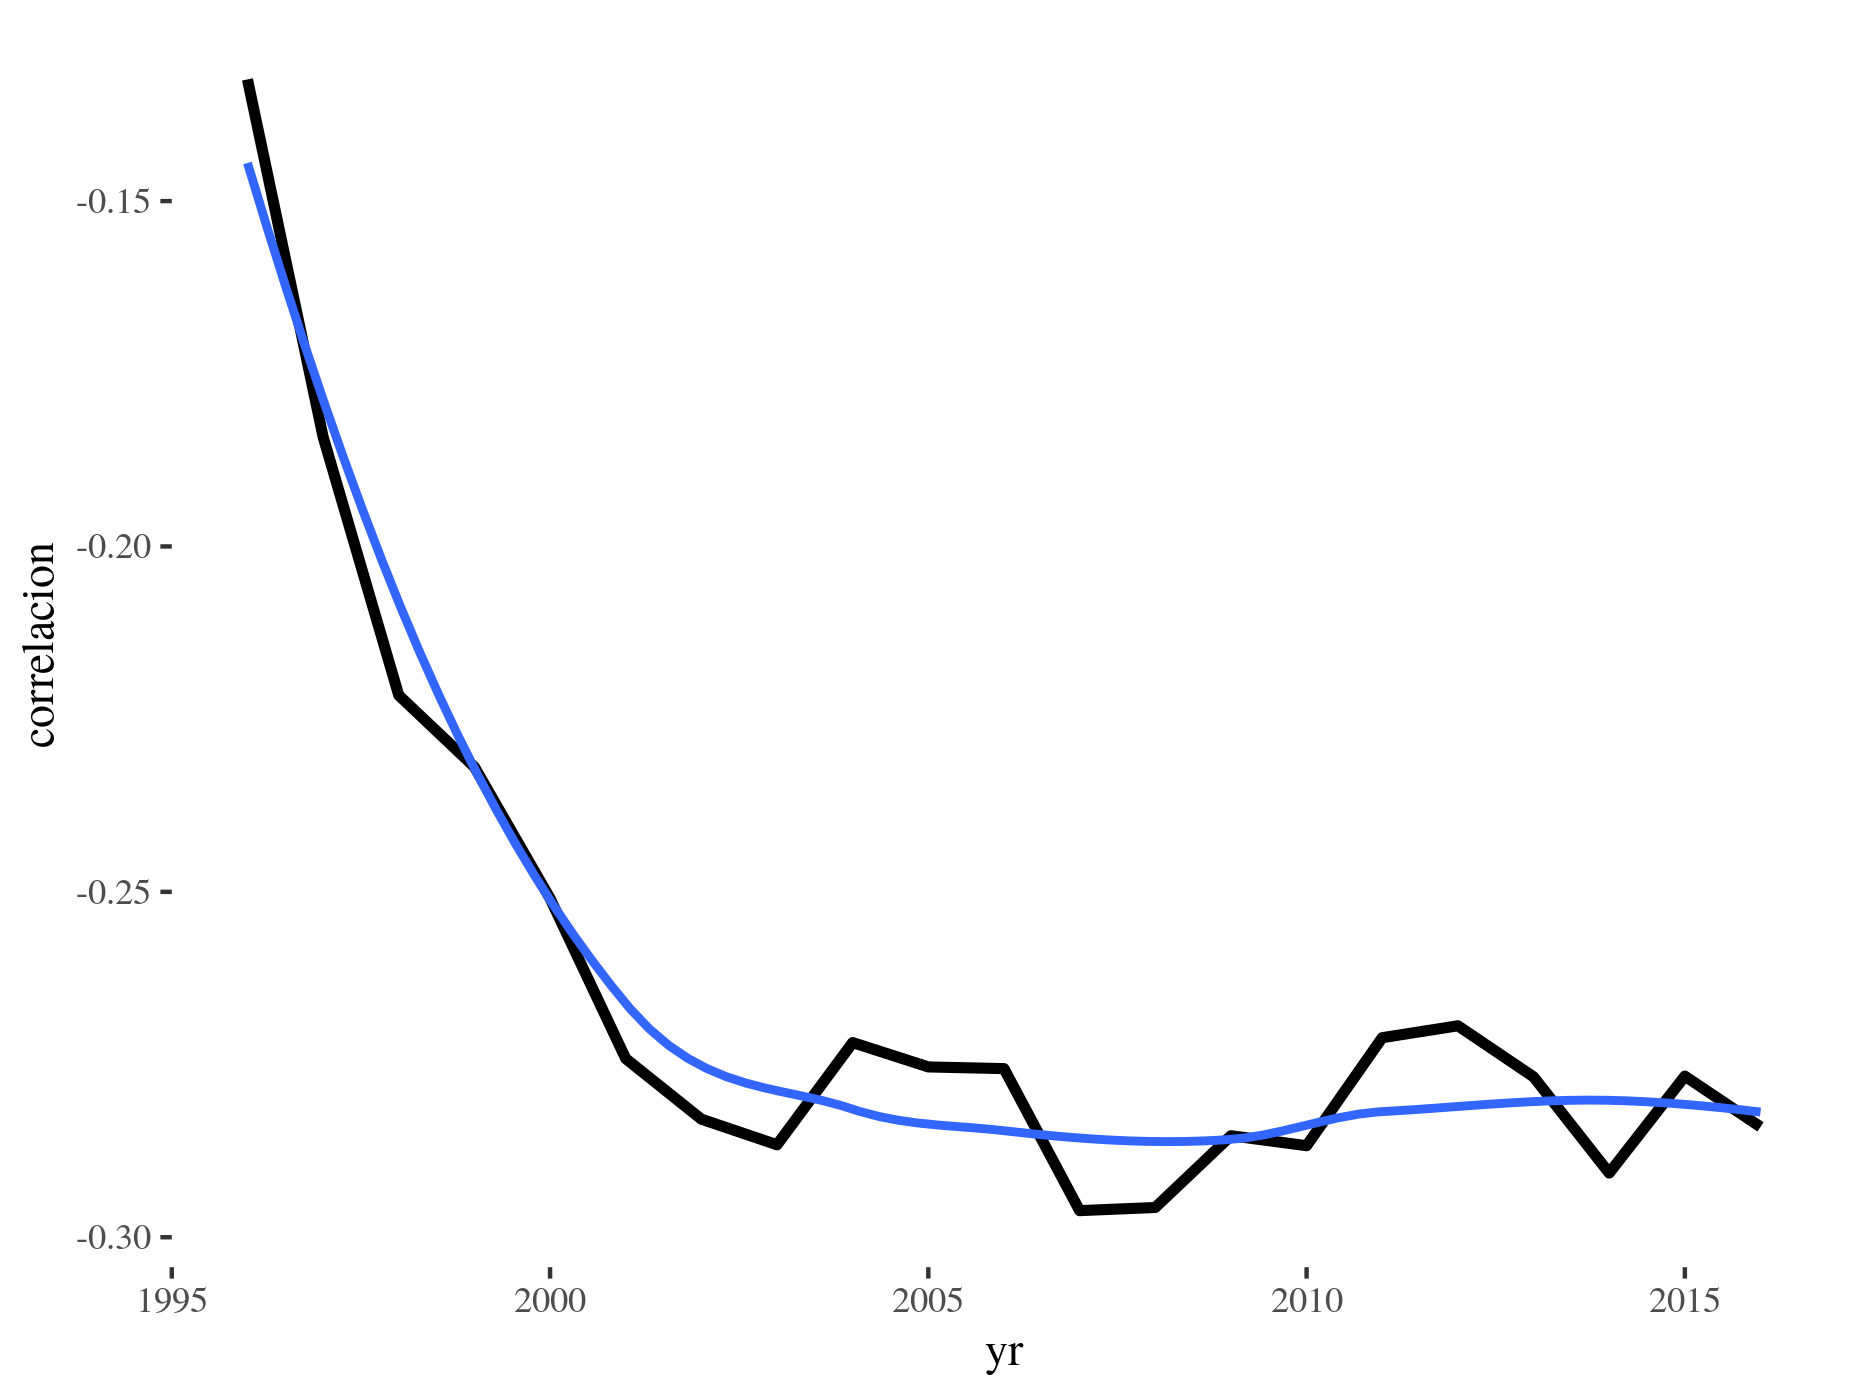
\includegraphics[width=.45\linewidth]{correlacion_x_yr}
	\label{fig:caracteristicas_yr-a}}
\subfigure[Coeficiente de clustering]{
    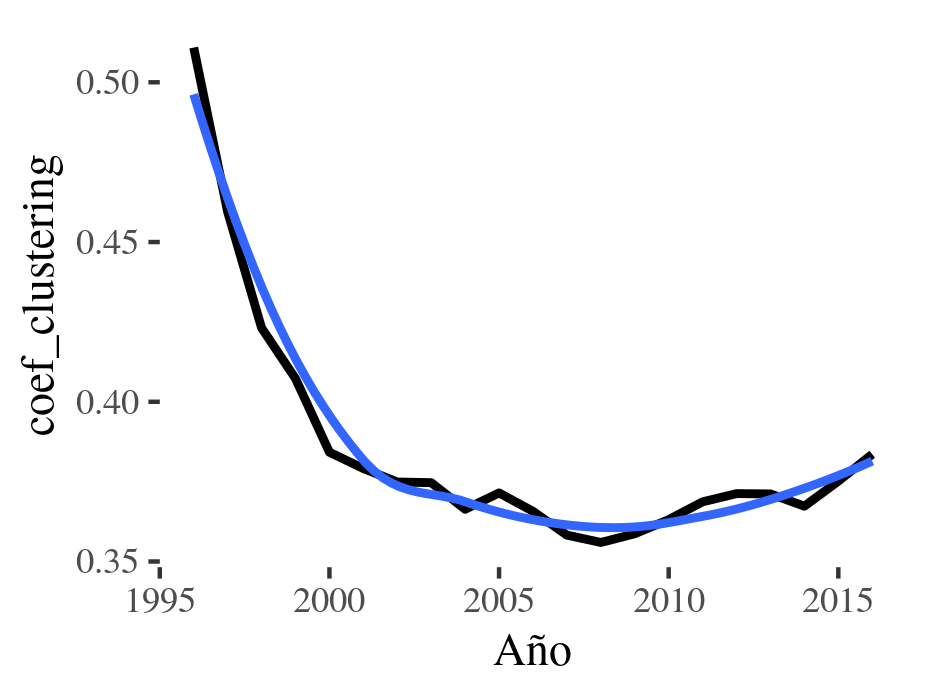
\includegraphics[width=.45\linewidth]{coef_clustering_x_yr}
    \label{fig:caracteristicas_yr-b}}
\caption{\textbf{Importaciones.} umbral 1\%, según año}
\label{fig:caracteristicas_yr}
\end{figure}


Como se puede observar, las características topológicas del grafo varían fuertemente en el período 2007-2009, durante la gran recesión económica, que se caracterizó por un aumento en el proteccionismo económico de ciertos países centrales, reflejado en el “Buy American”\footnote{http://edition.cnn.com/2009/POLITICS/02/05/senate.buy.american/index.html} o “Buy China”\footnote{https://economix.blogs.nytimes.com/2009/06/29/buy-china/}. 

La figura \ref{fig:caracteristicas_yr-a} muestra la caída de la correlación de grado en el año 2007, que implica una transición circunstancial hacia una economía menos selectiva. Es decir, un comercio internacional donde aumentan las relaciones de nodos de mayor grado con nodos de menor grado, respecto de las relaciones entre nodos de similar magnitud.

Por su parte, la figura \ref{fig:caracteristicas_yr-b} muestra como el coeficiente de clustering tiene una tendencia decreciente hasta 2008, para luego comenzar a crecer nuevamente. Esto se puede interpretar como una de-segmentación del comercio internacional hasta la crisis, con al cual comienza un proceso de re-segmentación. \\

\partitle{Distribución de los nodos}
A continuación se presenta la distribución de los nodos según ciertas medidas de centralidad a lo largo de los años, destacando aquellos países con mayores valores de centralidad. 


\begin{figure}
\centering
\subfigure[Grado, importaciones]{
    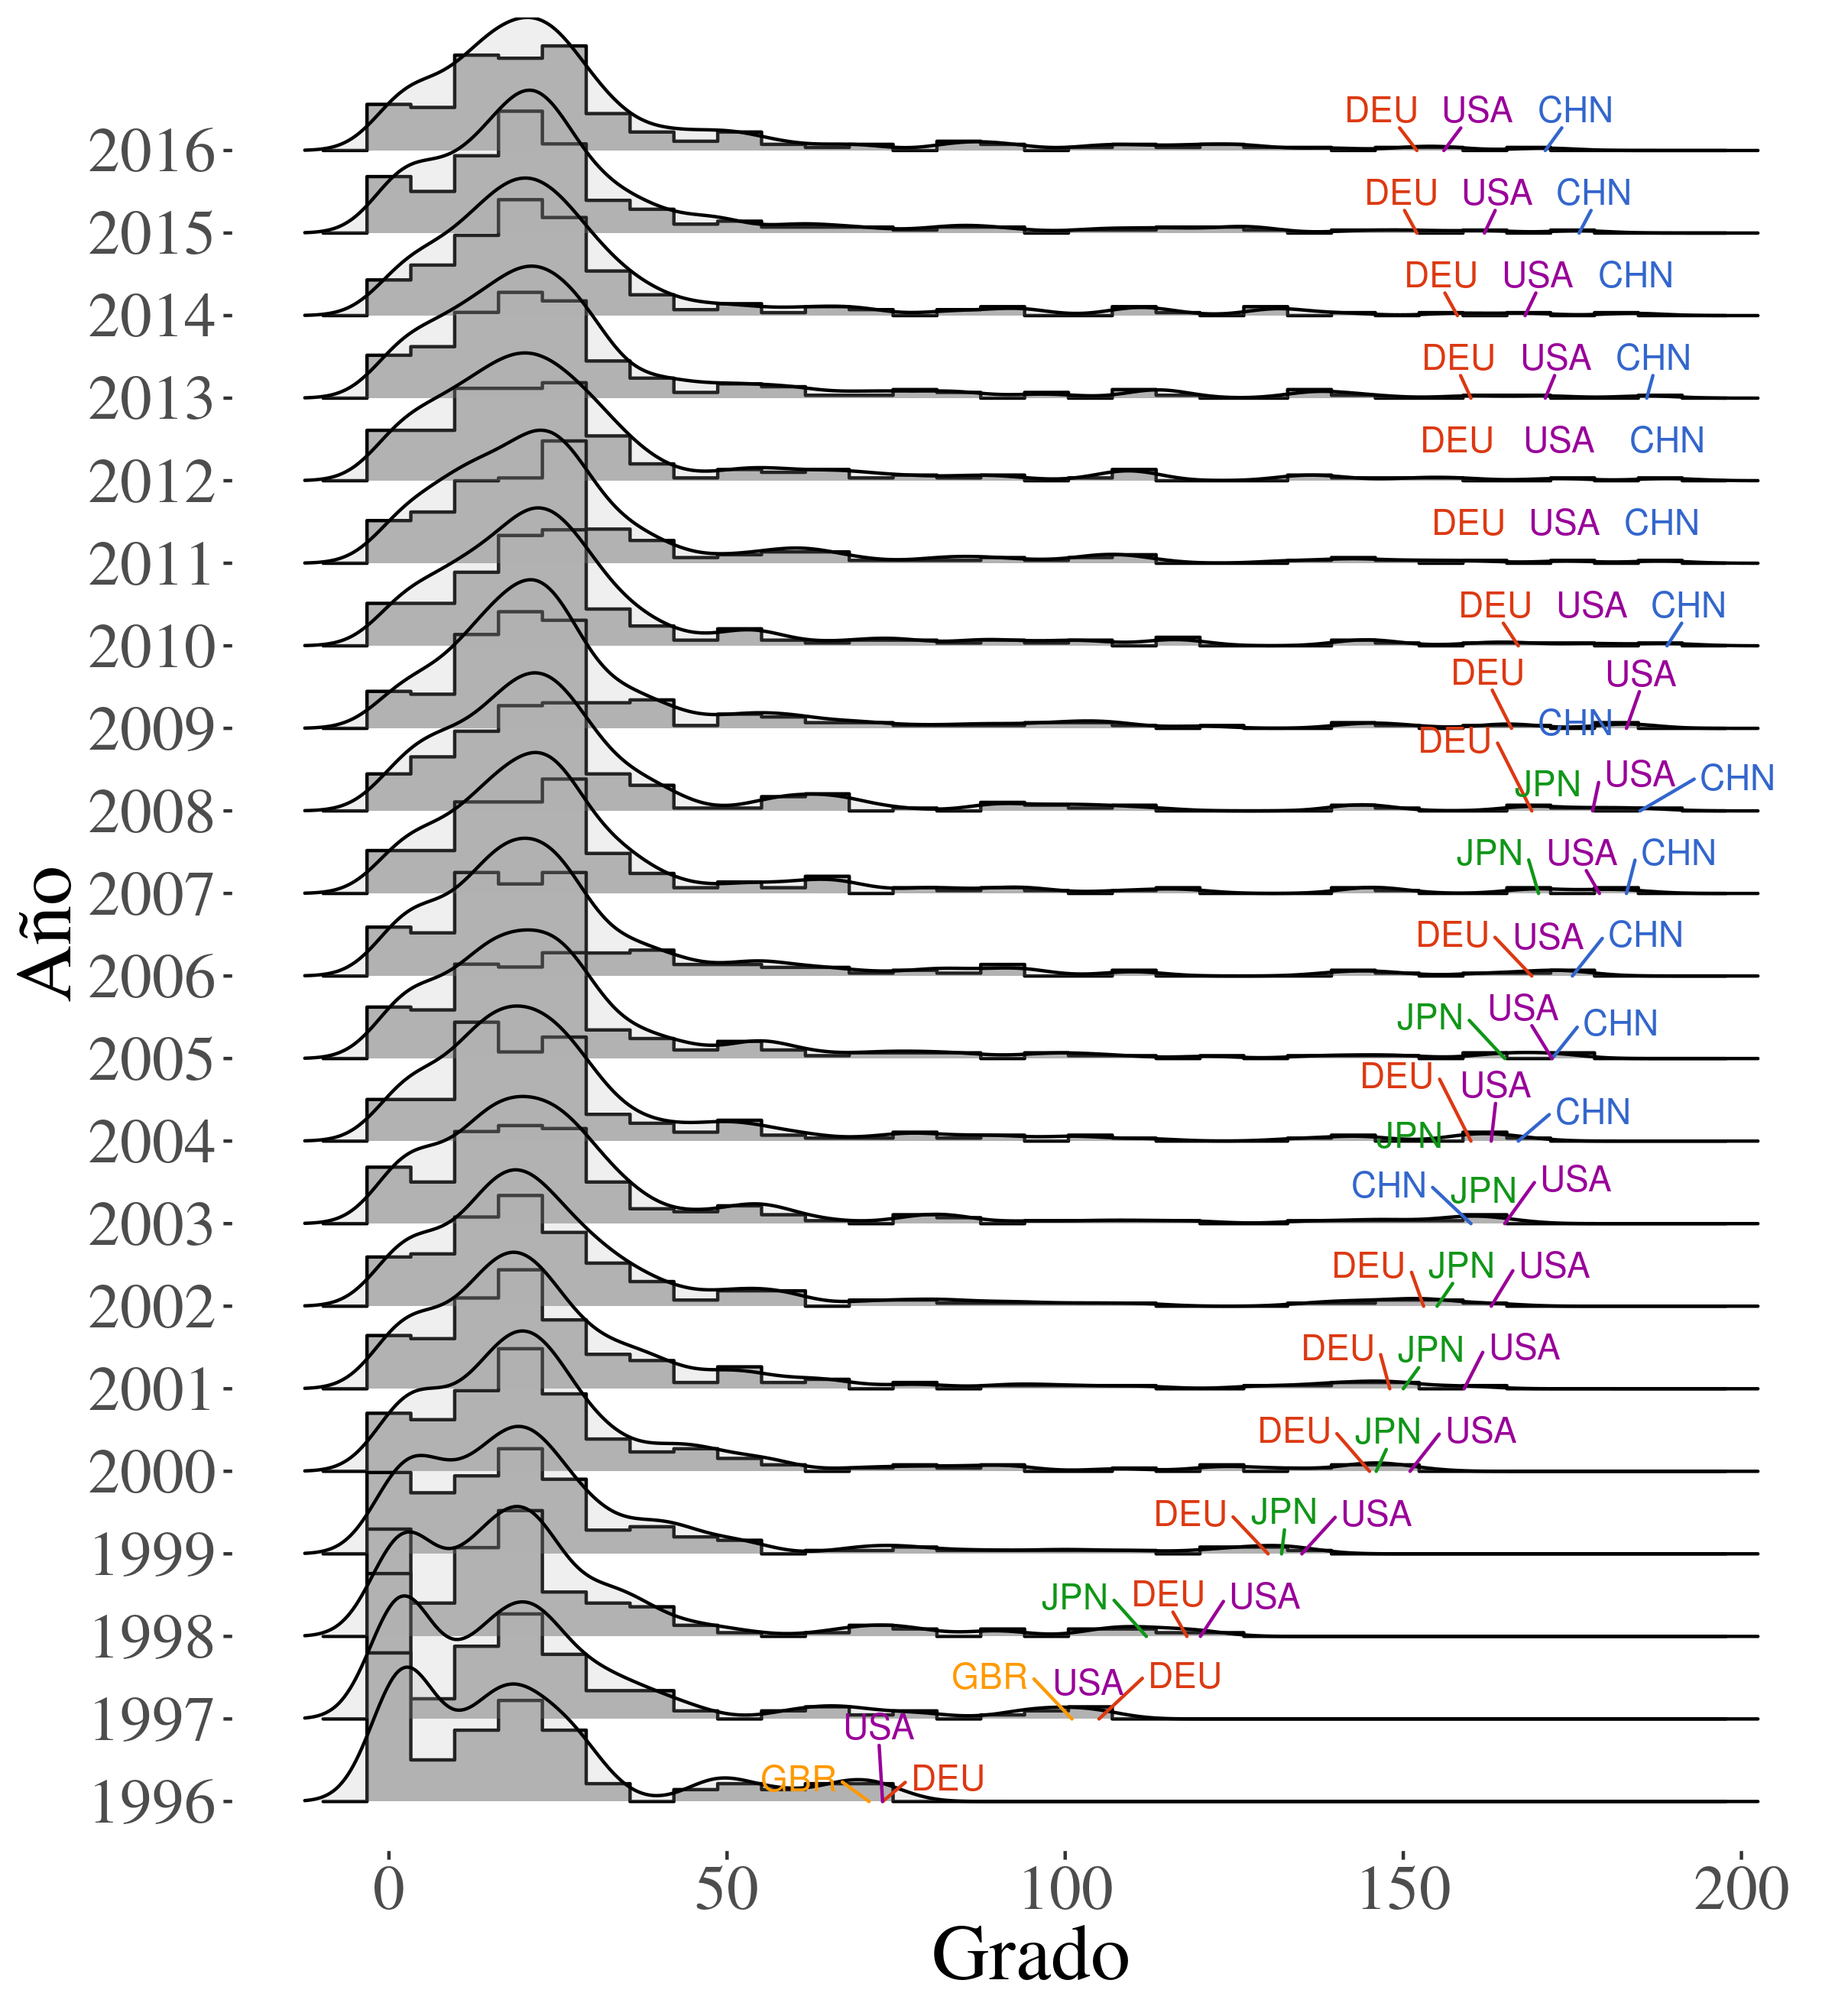
\includegraphics[width=.6\linewidth]{impo_densidad_degree_x_yr}
    \label{fig:distribuciones-a}}

\subfigure[Autovalor, exportaciones]{
    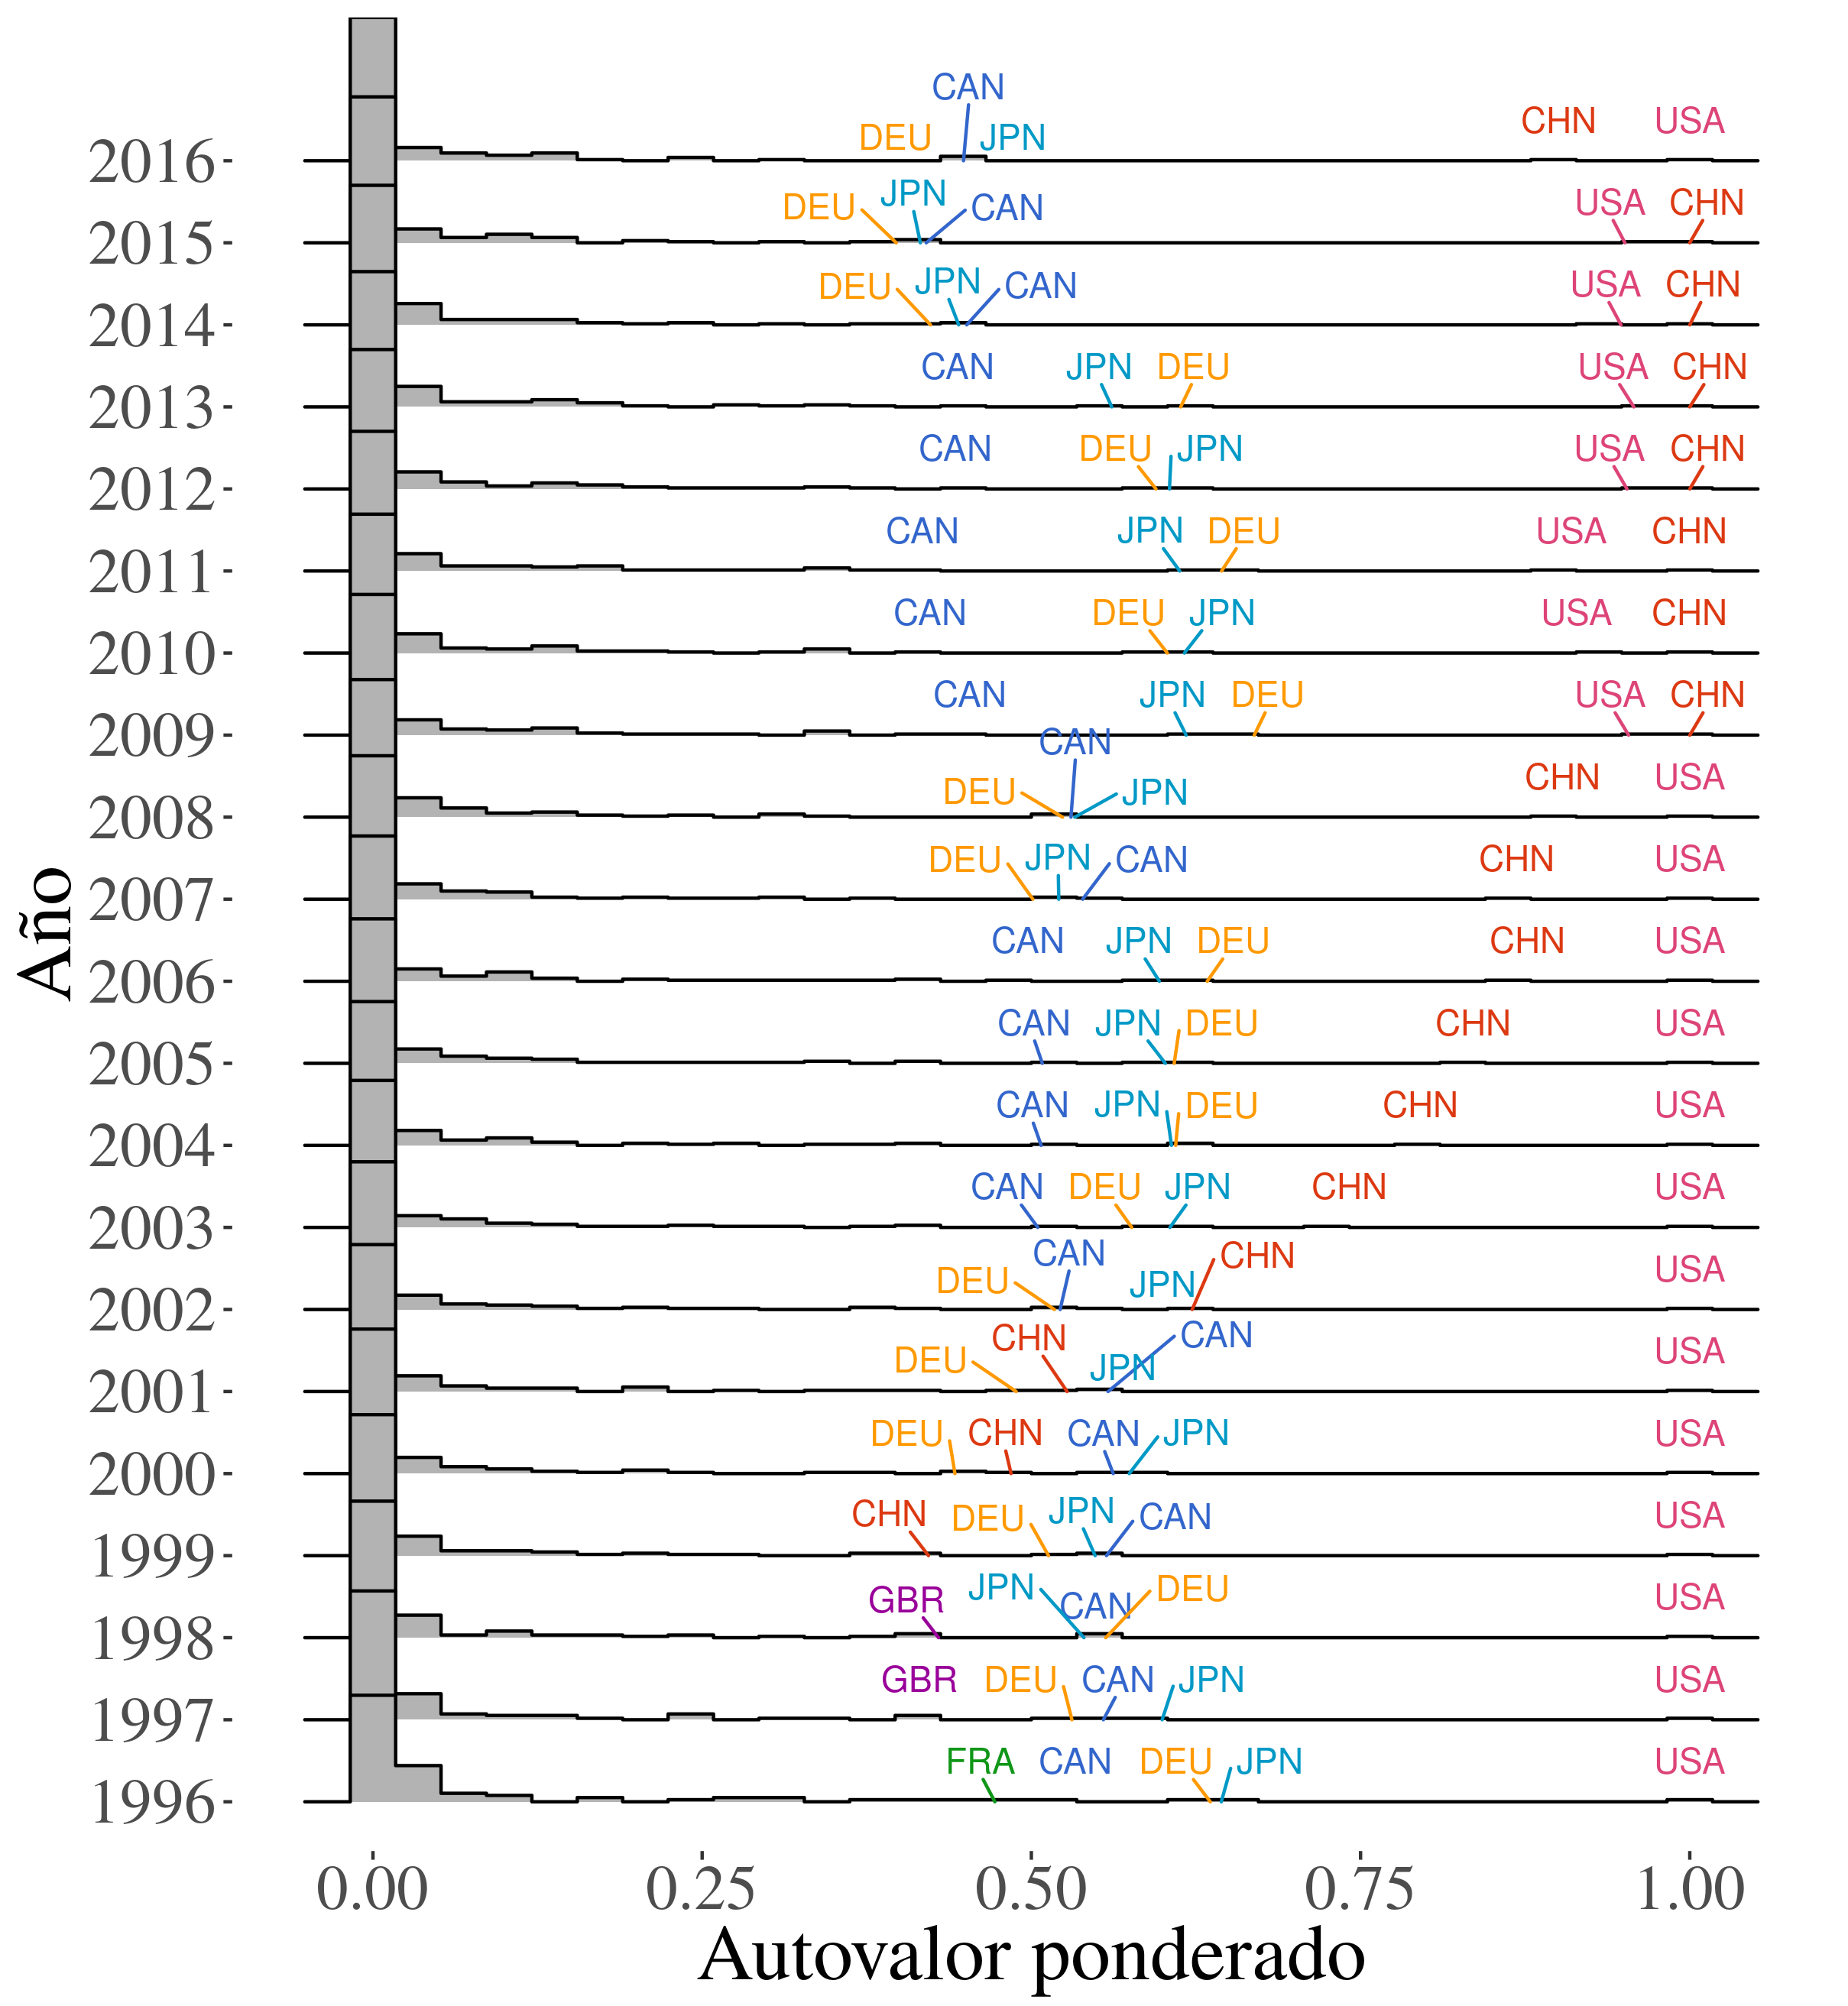
\includegraphics[width=.6\linewidth]{expo_densidad_autovalor_x_yr}
    \label{fig:distribuciones-b}}

%\subfigure[Autovalor ponderado, exportaciones]{
%    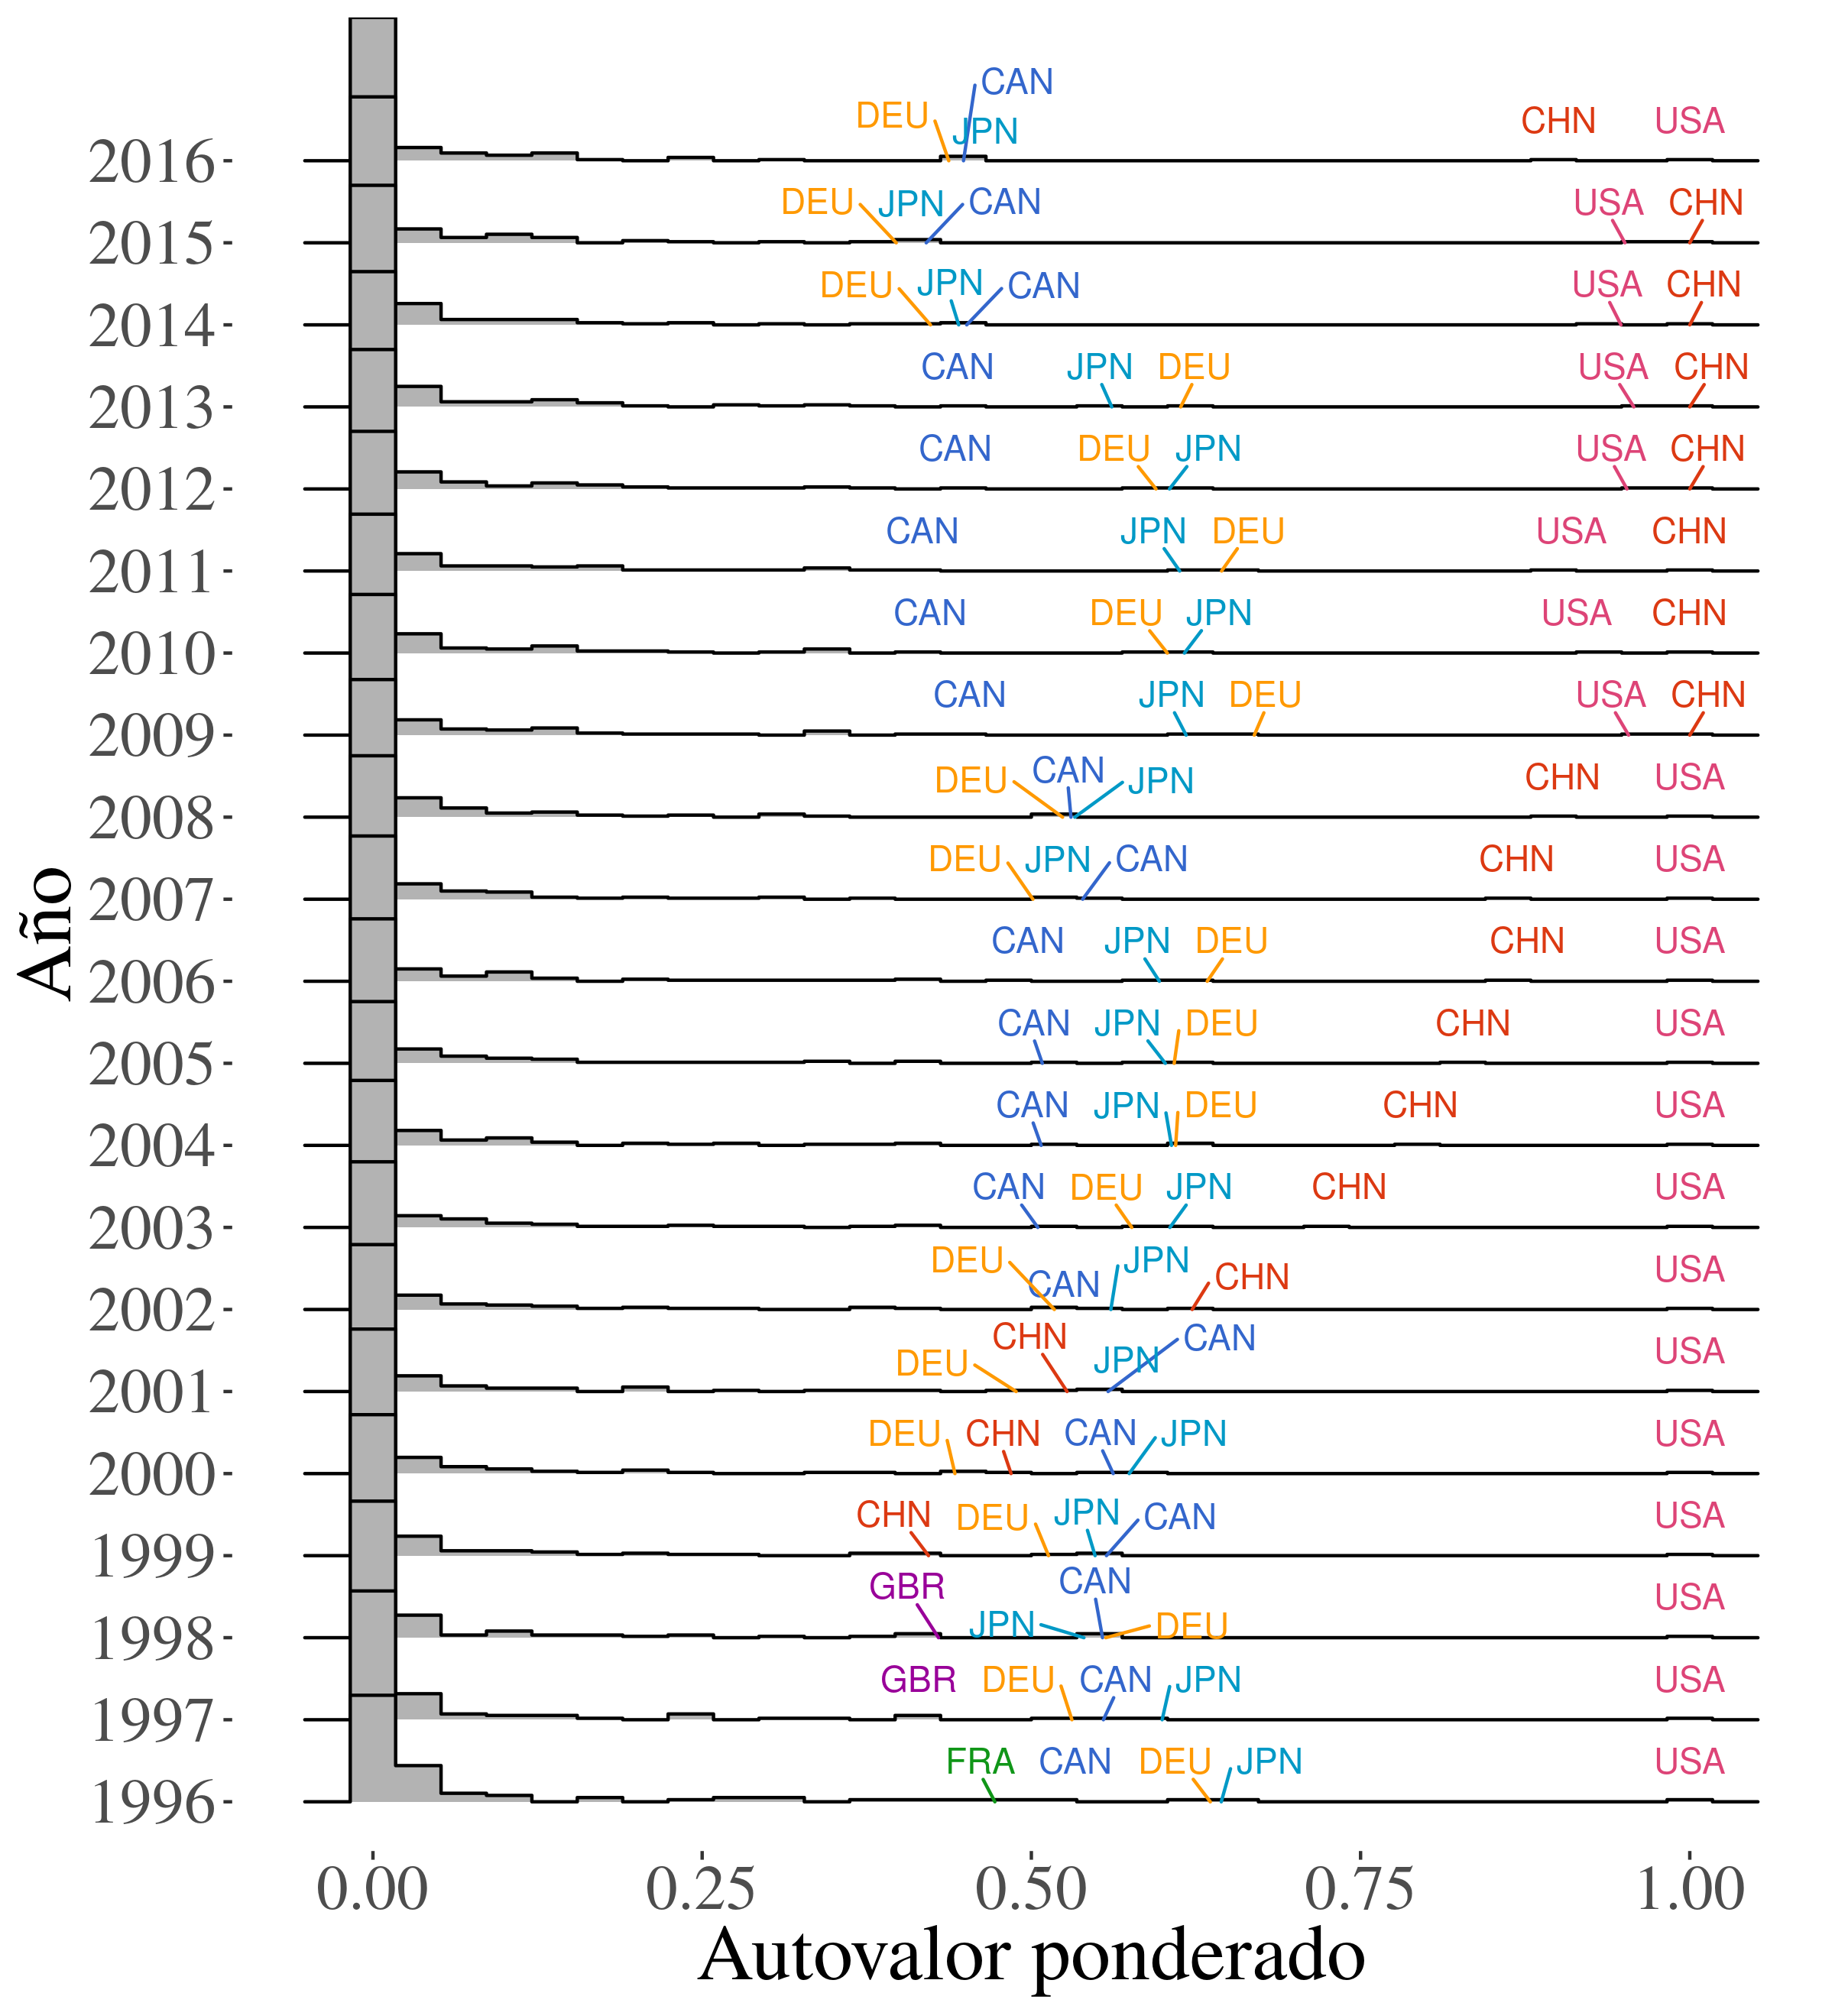
\includegraphics[width=.45\linewidth]{expo_densidad_USAvsCHN_autovalor_pond_x_yr}
%    \label{fig:distribuciones-c}}
%    
\caption{Distribución medidas de centralidad según año. umbral 1\%}
\label{fig:distribuciones}
\end{figure}



\begin{figure}
	\centering		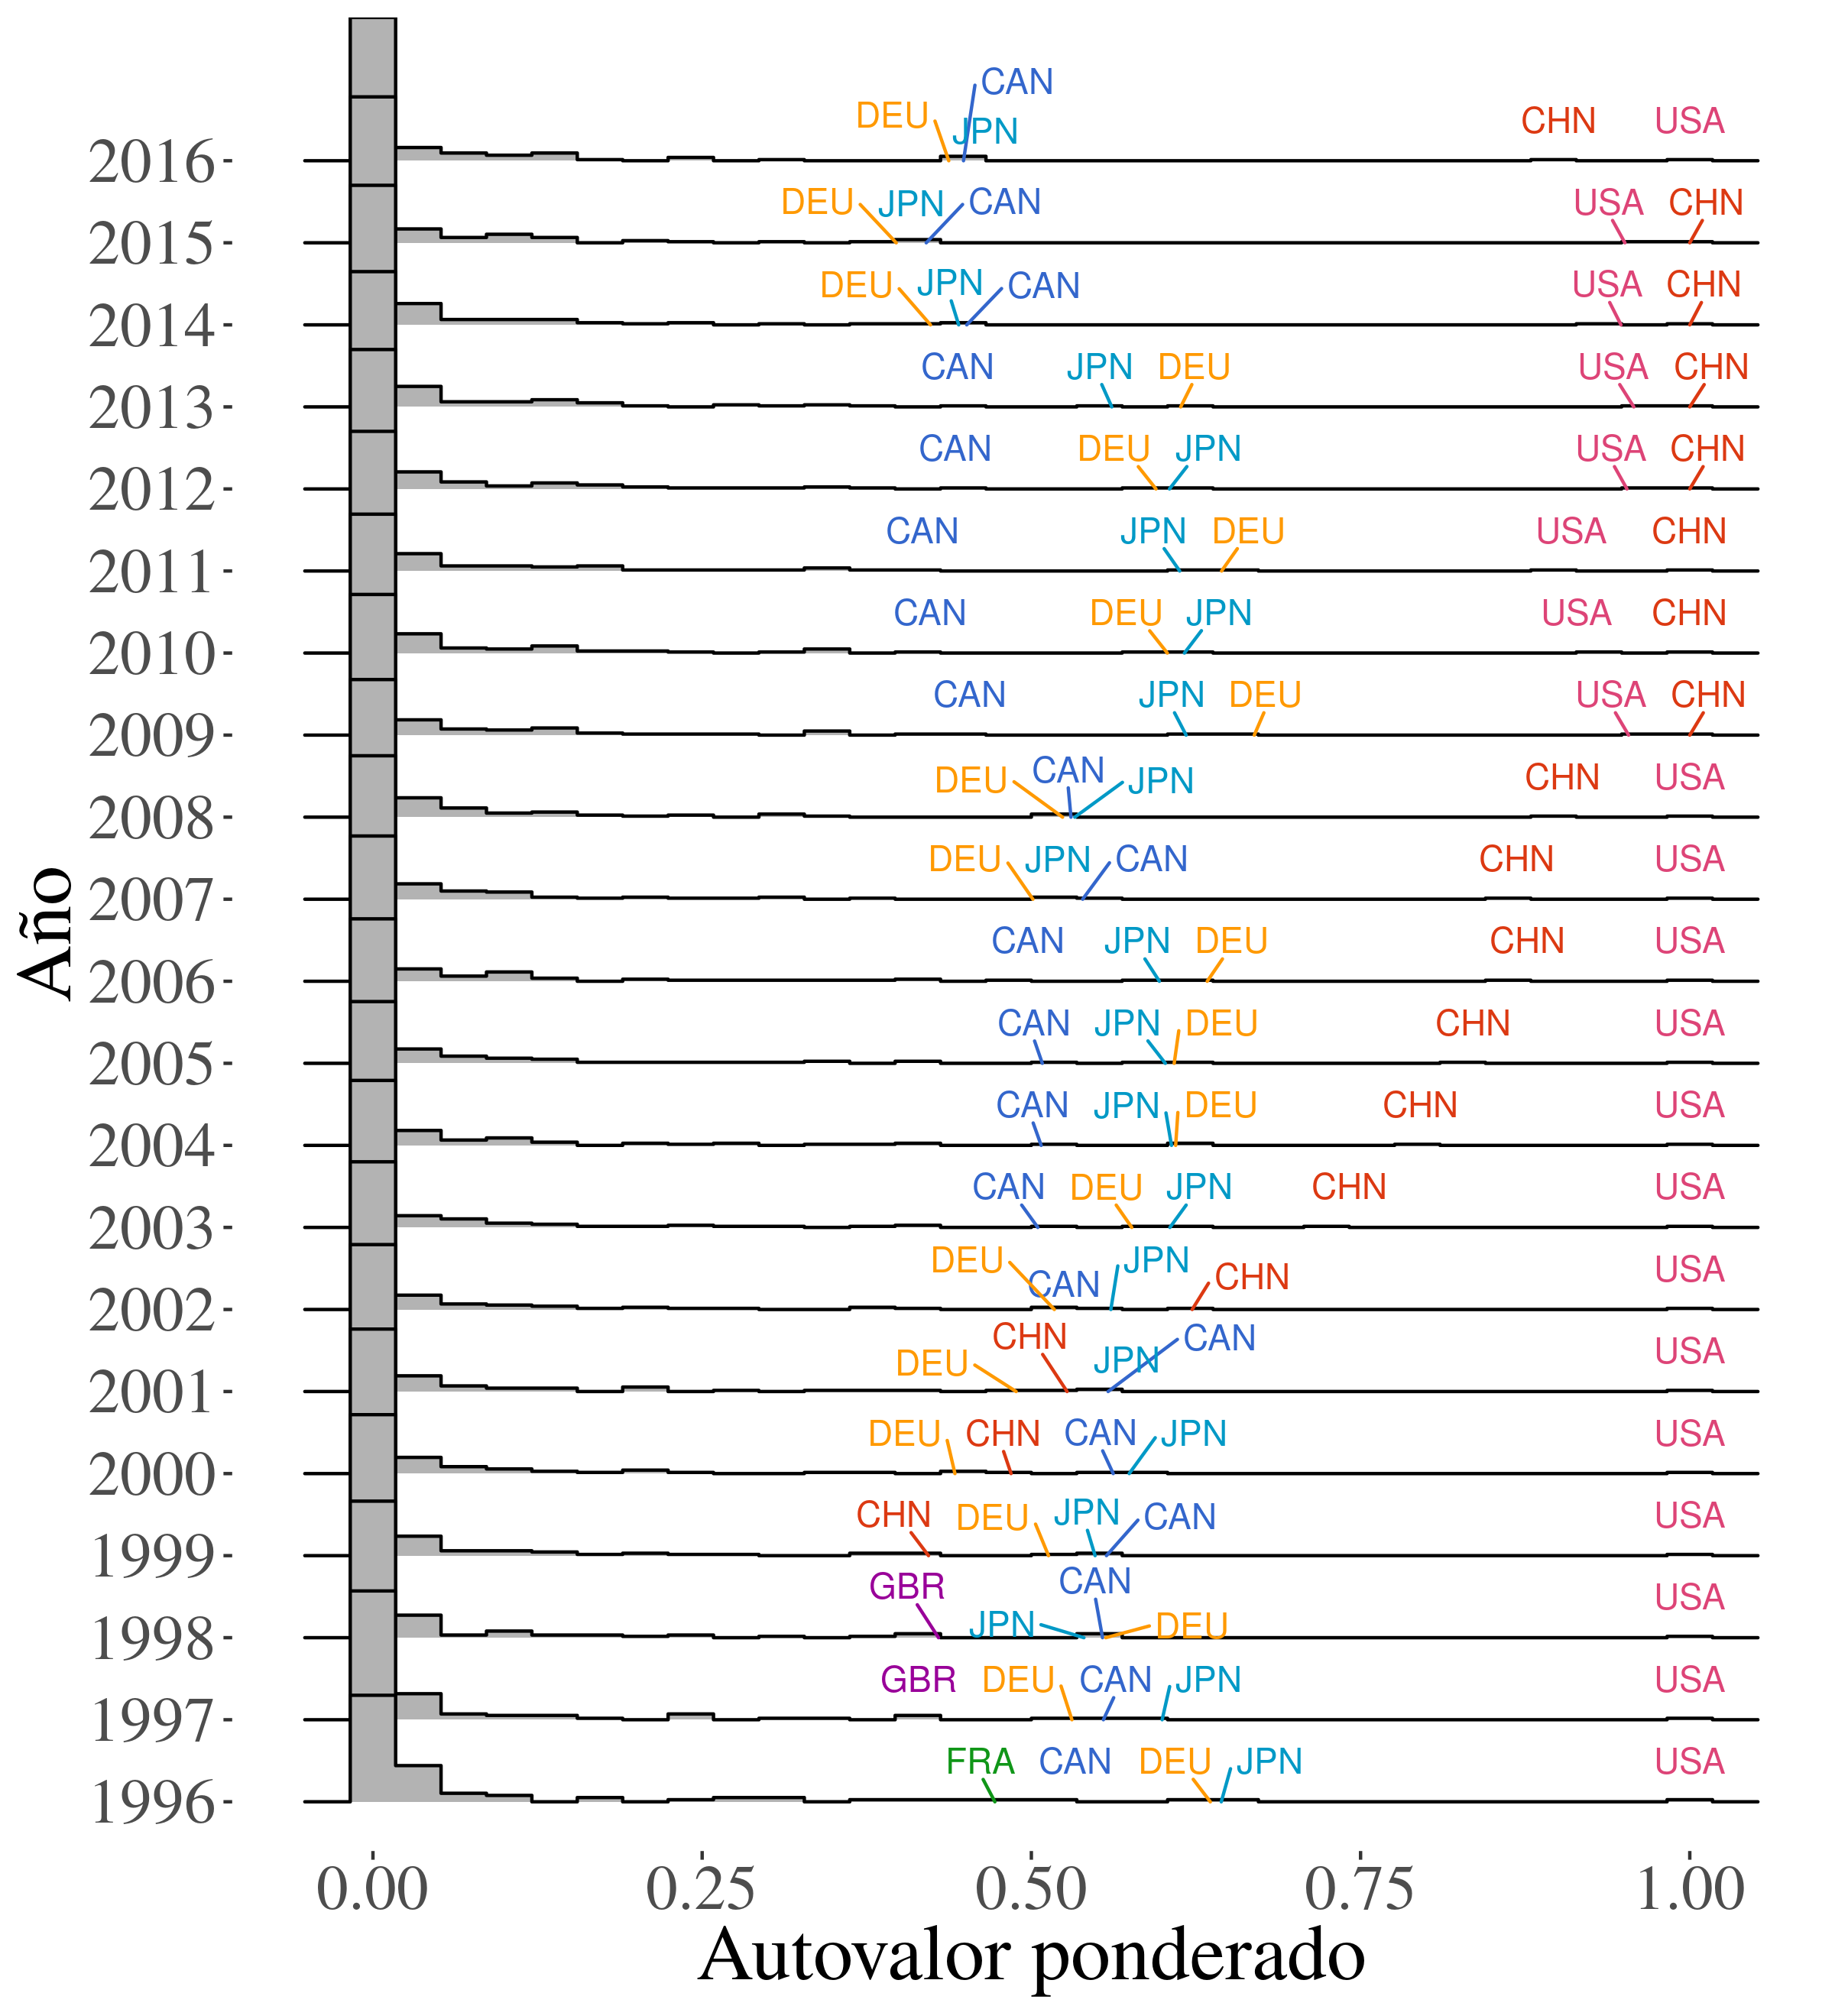
\includegraphics[width=.65\linewidth]{expo_densidad_USAvsCHN_autovalor_pond_x_yr}
	\caption{Distribución autovalor ponderado, exportaciones según año. umbral 1\%}
	\label{fig:distribuciones-c}
\end{figure}




En primer lugar, lo que se observa en la figura \ref{fig:distribuciones} es que la distribución de los nodos de acuerdo a las distintas medidas de centralidad no varía sustancialmente de año en año, ni en su rol como consumidores globales, ni en su rol como productores globales. Por su parte en \ref{fig:distribuciones-a} se observa la distribución de grado de los nodos del grafo de importaciones, donde se ve como los tres países de mayor grado tienden a alejarse del centro de masa de la distribución. Este podio se disputa entre Alemania, Japón, Estados Unidos y, a partir del 2002, China, quien a su vez tiende a alejarse de éstos posteriormente. Por su parte, la figura \ref{fig:distribuciones-b} marca el rol de consumidores globales. Aquí, mientras hasta 2007 Estados Unidos y Gran Bretaña ocupan los lugares principales en la centralidad de autovalor, a partir de este año comienza a tener un rol más destacado Francia, los países bajos, y luego China.      

Es de resaltar el aumento en la centralidad de China para el comercio internacional, tanto como productor como consumidor. En particular, este país desplaza a Estados Unidos de ser el nodo de mayor centralidad en muchas medidas. Por ejemplo, la figura \ref{fig:distribuciones-c} para el caso del autovalor ponderador por el valor del intercambio, Estados Unidos ocupa el primer lugar hasta el año 2006, para luego ser reemplazado por China, un país que diez años antes tenía un valor de centralidad cuatro veces menor al de Estados Unidos. En ese mismo año China también pasa a ocupar el primer lugar en dicha métrica para el grafo de las importaciones. La medida de centralidad del autovalor es particularmente relevante, sobretodo todo ponderada por el valor de las transacciones, porque considera no sólo la importancia del nodo, sino también la importancia de aquellos nodos con que se relaciona. En este sentido, se destaca el rol de México, Japón, Canadá, junto con China y Estados Unidos como grandes productores mundiales, a la vez que aparece, sobre los últimos años, Corea como una nueva potencia en este aspecto.  

\subsubsection{Análisis de largo plazo}

Otro análisis que resulta interesante es la evolución de la red en un período de largo plazo. Esto nos permite encontrar los cambios estructurales del comercio internacional, a la vez que da cuenta de qué elementos de la topología de la red son robustos, y cuales contienen una tendencia histórica. 
Para esto, tomamos la serie elaborada por \cite{Gleditsch2002}, que reúne información del comercio internacional entre 1948 y 2000. 
A continuación se analizan los elementos estructurales de la red, para luego analizar la evolución de algunos países seleccionados dentro del grafo

\partitle{Estructura de la red}
Como se observa en la figura \ref{fig:metricas_LP}, en la red ocurren importantes cambios en el período que va de 1948 al año 2000. 
La figura \ref{fig:metricas_LP-a} muestra la evolución del coeficiente de clustering de la red. Este, como se mencionó previamente, indica la tendencia de la red a formar vecindarios bien delimitados. La fuerte caída durante las décadas del cincuenta y sesenta reflejan la nueva división internacional del trabajo, en dónde las relaciones comerciales se alejan del regionalismo, y el comercio inter-continental aumenta en volumen. En concreto, esta expresando la incorporación de Asia como productor de mercancías para el mercado mundial. 
\par
La figura \ref{fig:metricas_LP-b} muestra la evolución del coeficiente de correlación de grado. Este indica el grado de homofilia de la red, es decir, la tendencia de los nodos de mayor grado a conectarse con otros nodos de similares características. Recordemos que al tomar valores negativos, esta correlación indica una tendencia de los países de mayor grado a relacionarse con países de menor grado. La caída de este valor en las décadas del cincuenta y sesenta expresa un incremento en esta característica de la red.  

\begin{figure}[h!]
	\centering
	\subfigure[Coeficiente de Clustering, importaciones]{\label{fig:metricas_LP-a}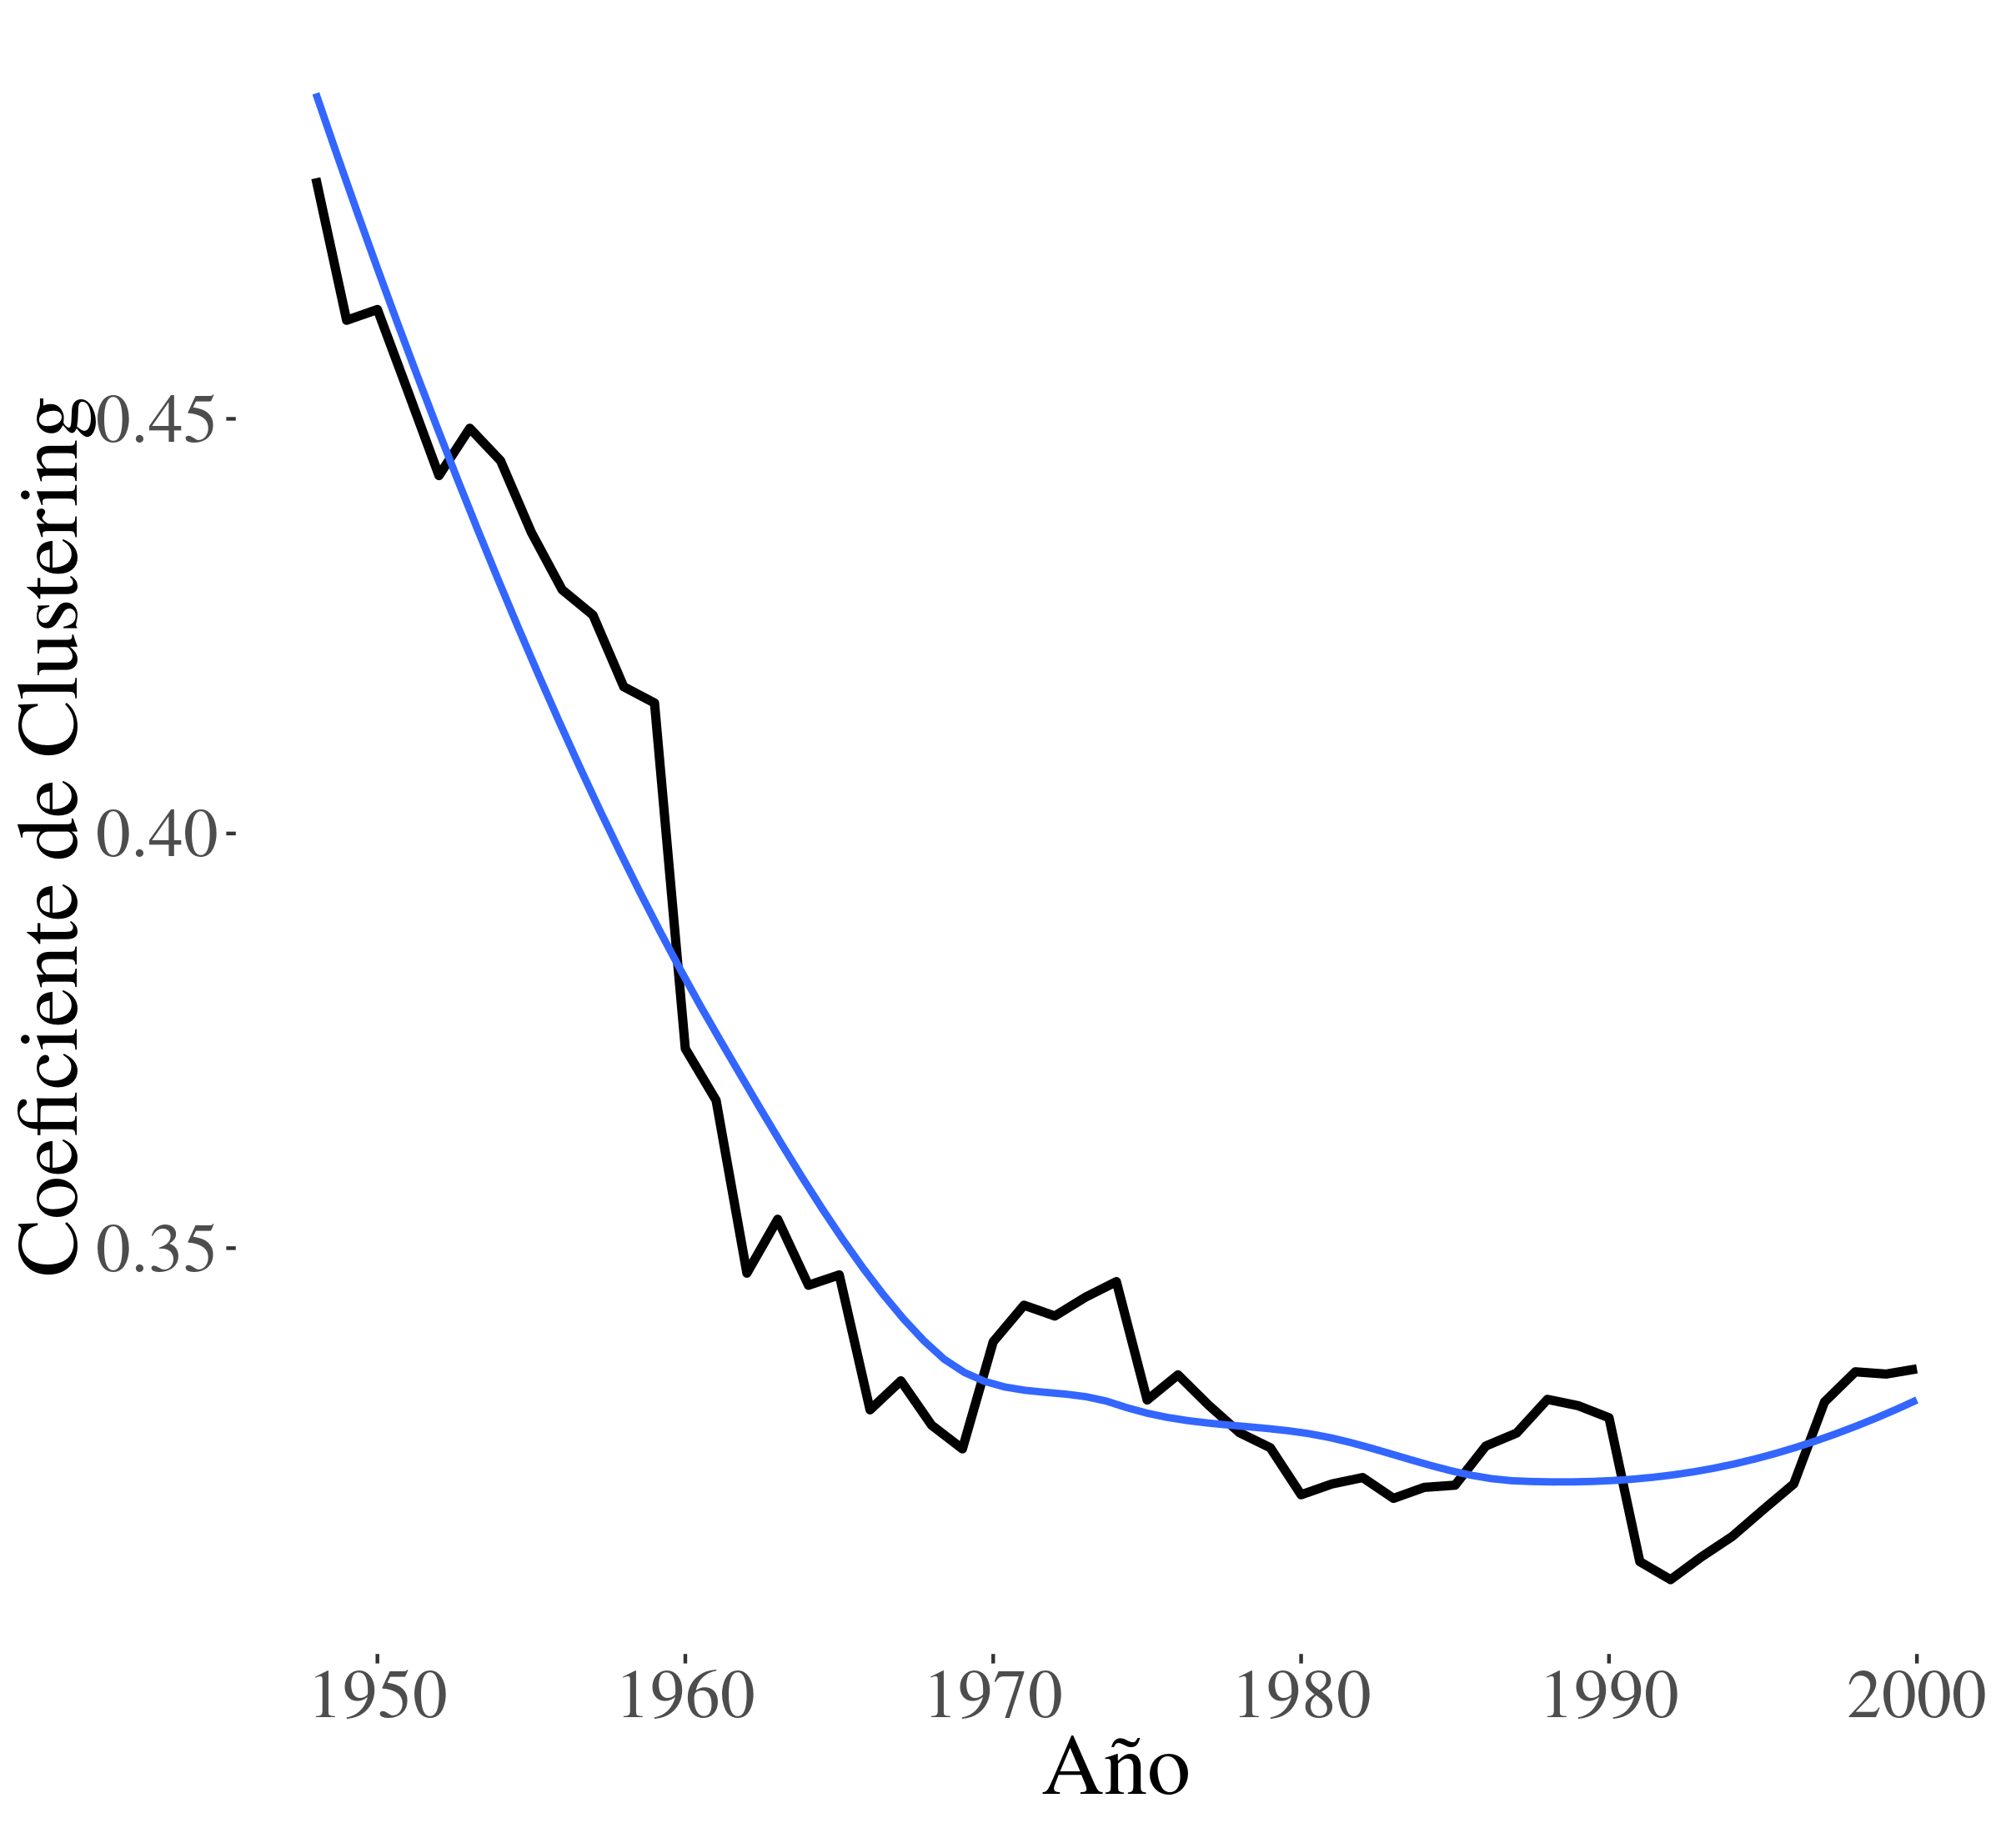
\includegraphics[width=.48\linewidth]{1950_2000_coef_clustering_x_yr}}
	\subfigure[Correlación de grado, importaciones]{\label{fig:metricas_LP-b}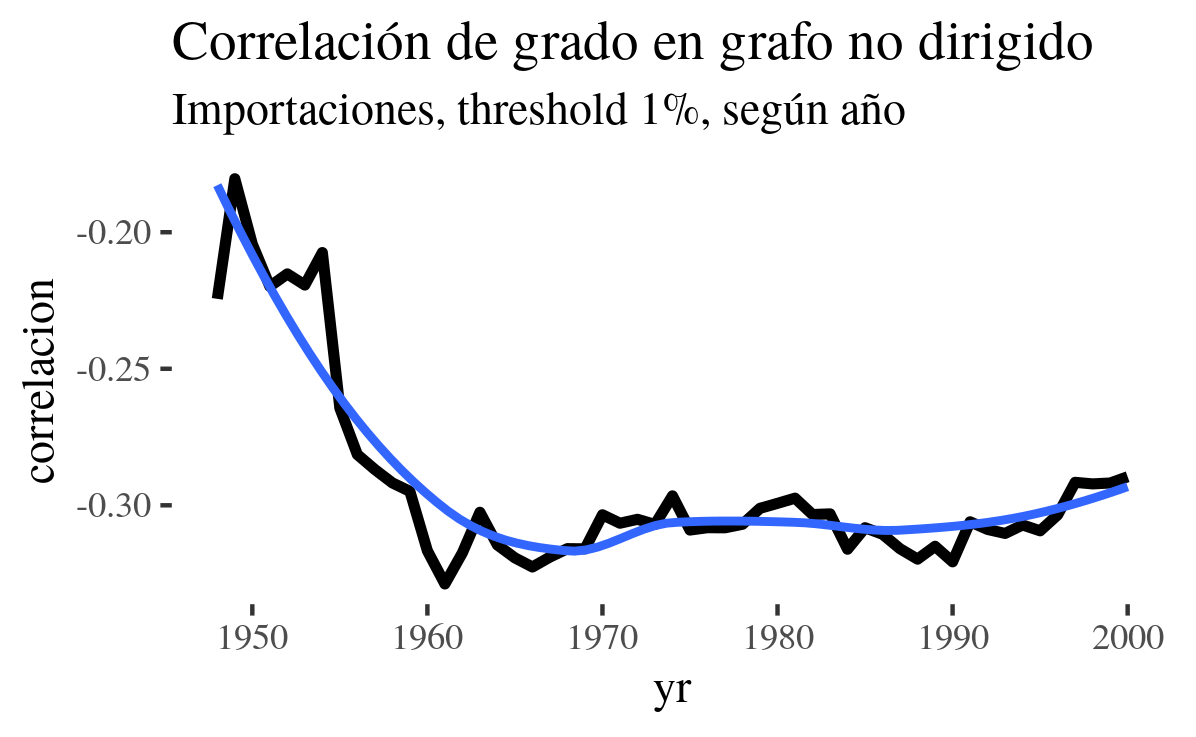
\includegraphics[width=.48\linewidth]{1950_2000_correlacion_x_yr}}
	\caption{Evolución de la estructura de la red. Impo. Umbral 1\%}
	\label{fig:metricas_LP}
\end{figure}

Estas medidas refieren a características generales del grafo. También es posible analizar, dentro del grafo, el movimiento en la centralidad de subconjuntos del mismo. En particular, en la figura  \ref{fig:centralidad_LP} se muestra la evolución de la centralidad promedio por continente para las medidas de autovalor, cercanía y grado. En primer lugar, resalta la robustez de la centralidad de cercanía, que evoluciona uniformemente para todos los continentes. La disminución de esta medida indica un crecimiento del tamaño de la red \footnote{ Que parcialmente puede deberse a la incorporación de nuevas fuentes de información, en particular para los años 1949, 1960 y 1991}. \par
La centralidad de autovalor, por su parte, muestra un cambio importante en el rol de los países en la economía mundial. Mientras que Oceanía pasa del segundo al quinto lugar en el período, Asia hace lo opuesto, marcando la incorporación al mercado mundial de este continente como productor de mercancías.  Africa y América, por su parte, si bien siguen un distinto recorrido a lo largo del período, comienzan y terminan el mismo con valores muy similares. Europa mantiene la mayor centralidad promedio a lo largo de todo el período, en las tres métricas. Por último, el recorrido de Asia y Oceanía es similar para la centralidad de grado.

\begin{figure}[h!]
	\centering		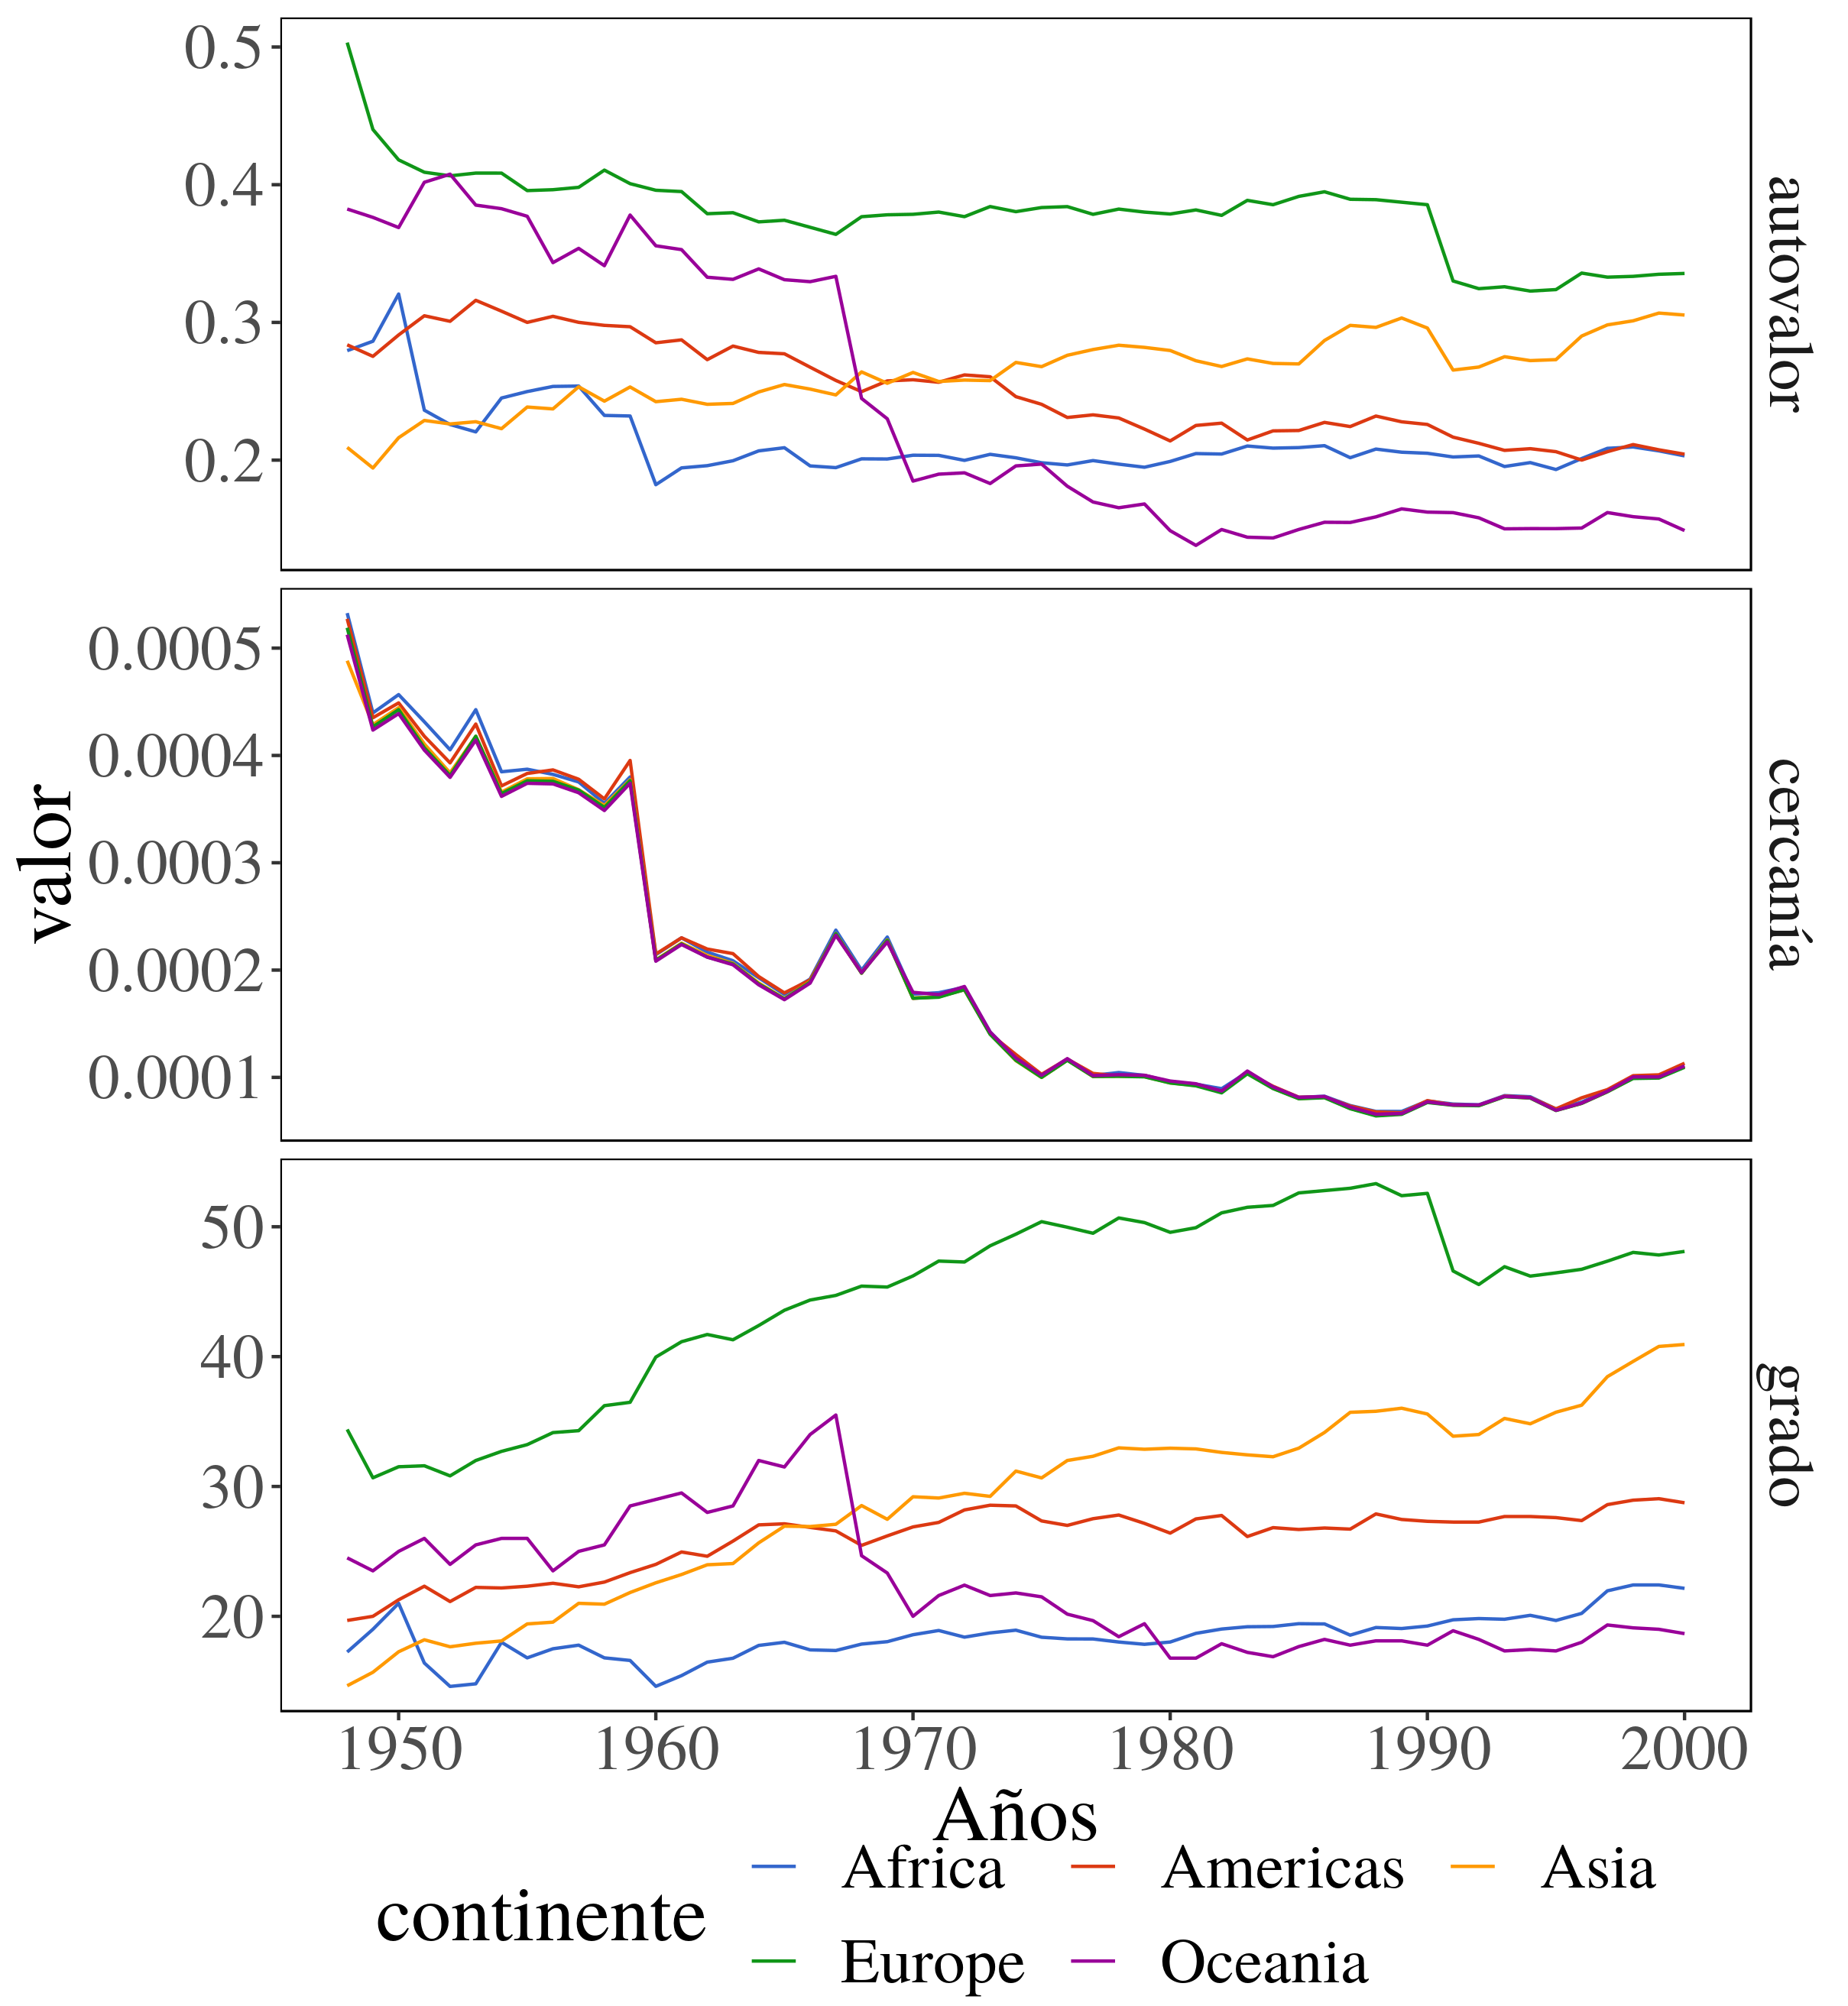
\includegraphics[width=0.75\linewidth]{1950_2000_continent_all}
	\caption{Evolución de la centralidad promedio por contiente. Impo. Umbral 1\%}
	\label{fig:centralidad_LP}
\end{figure}

\partitle{Evolución de los países}
Otra característica interesante del análisis de grafos es que permite seguir la evolución de un país en particular dentro del mismo, de forma tal que se puede observar la evolución de la centralidad de algunos nodos en el tiempo. \par
En la figura \ref{fig:paises_LP} se muestra la distribución de las medidas de grado y de autovalor ponderado, y se marca la posición de México Brasil y Argentina en dicha distribución. 
En \ref{fig:paises_LP-a} observamos la cantidad de conexiones de cada país en el grafo de las importaciones. Aquí se observa como México comienza la serie en la moda de la distribución de grado, mientras que Brasil y Argentina se encuentran a la derecha de la misma. En la evolución se vé como la distribución se convierte en más leptocúritca, y, por un lado Brasil incrementa la cantidad de nodos considerablemente, mientras que por otro lado Argentina mantiene a lo largo de toda la serie la misma cantidad de socios comerciales. Por su parte, México, pasa a ubicarse en la cola derecha de la distribución, más cercano a la Argentina. 
En \ref{fig:paises_LP-b} se observa el autovalor ponderado por el volumen comerciado. Considerando esta medida, la evolución pareciera ser diferente. Mientras Argentina se mantiene en el mismo lugar de la distribución, Brasil se repliega hacia valores similares a los Argentinos, y México se despega de la moda de la distribución a partir de los años noventa. Al considerar no solo el grado, sino también el grado de los vecinos, y el volumen comerciado, se destaca el proceso de la \textit{Maquila Mexicana}, en dónde el comercio entre este país y Estados Unidos, un nodo sumamente importante, es muy difundido. 

\begin{figure}[h!]
	\centering
	\subfigure[Grado]{\label{fig:paises_LP-a}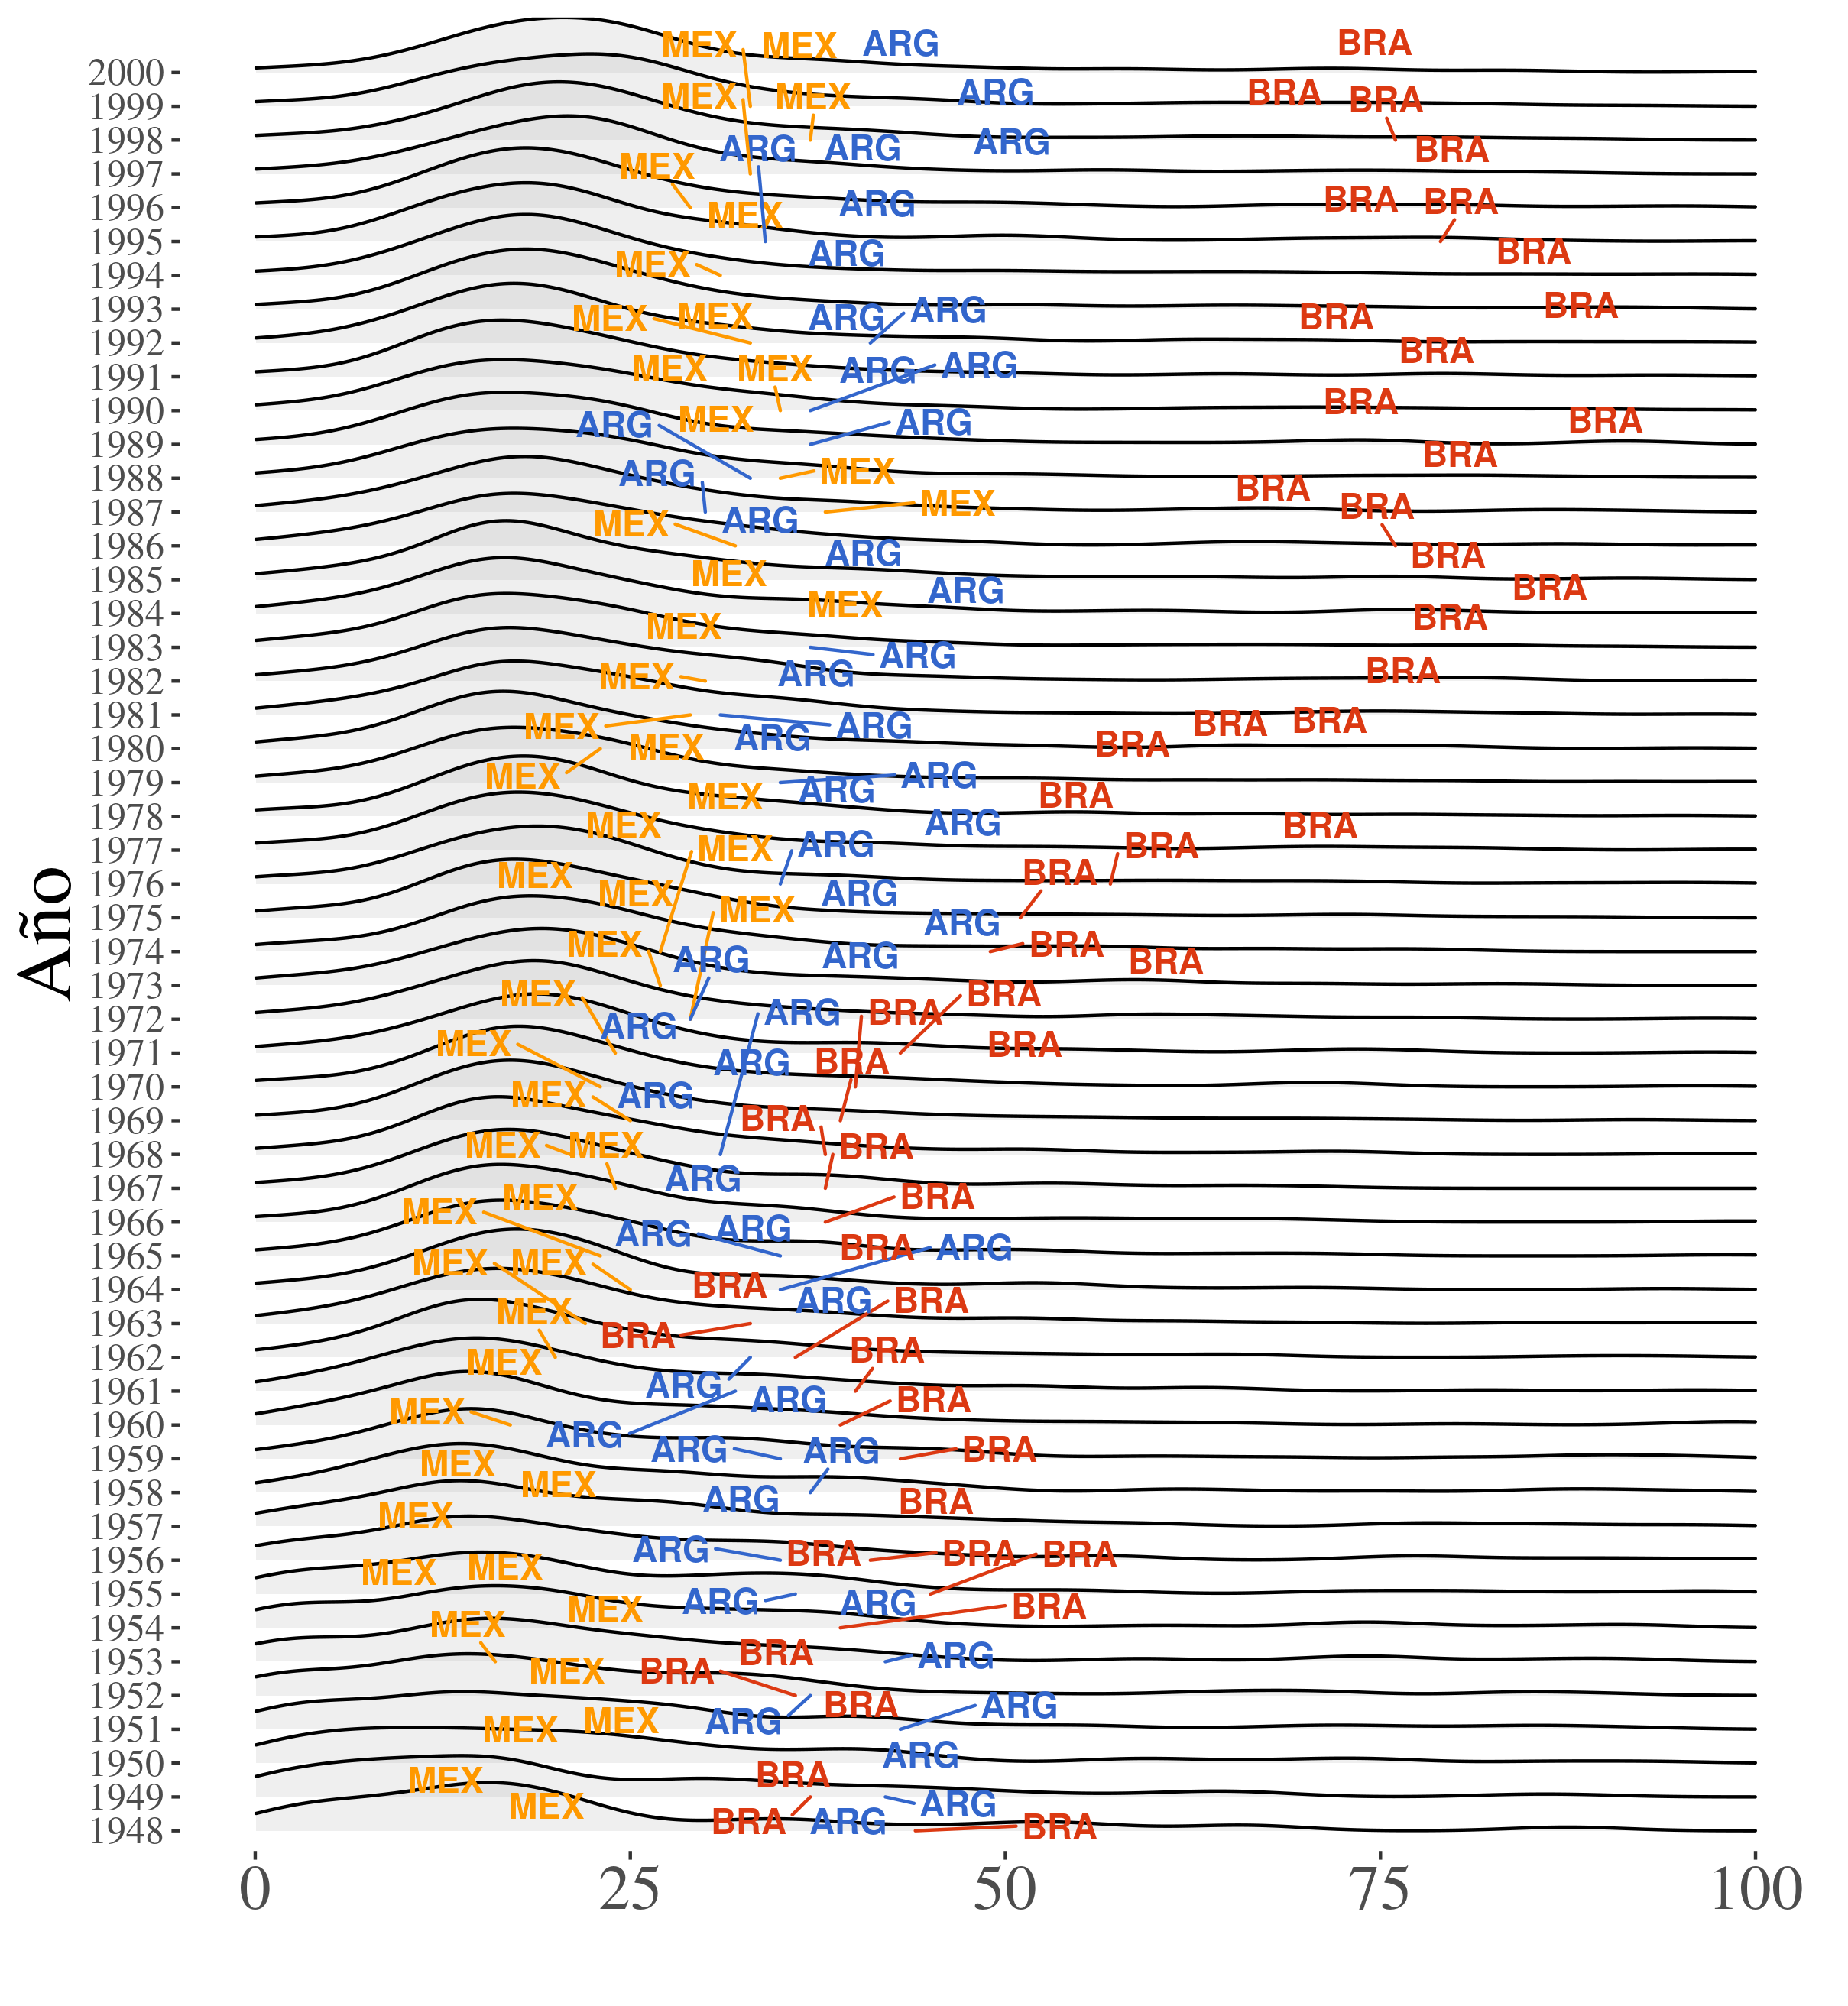
\includegraphics[width=0.7\linewidth]{1950_2000_impo_densidad_ARG_BRA_MEX_grado}}
	\subfigure[Autovalor Ponderado]{\label{fig:paises_LP-b}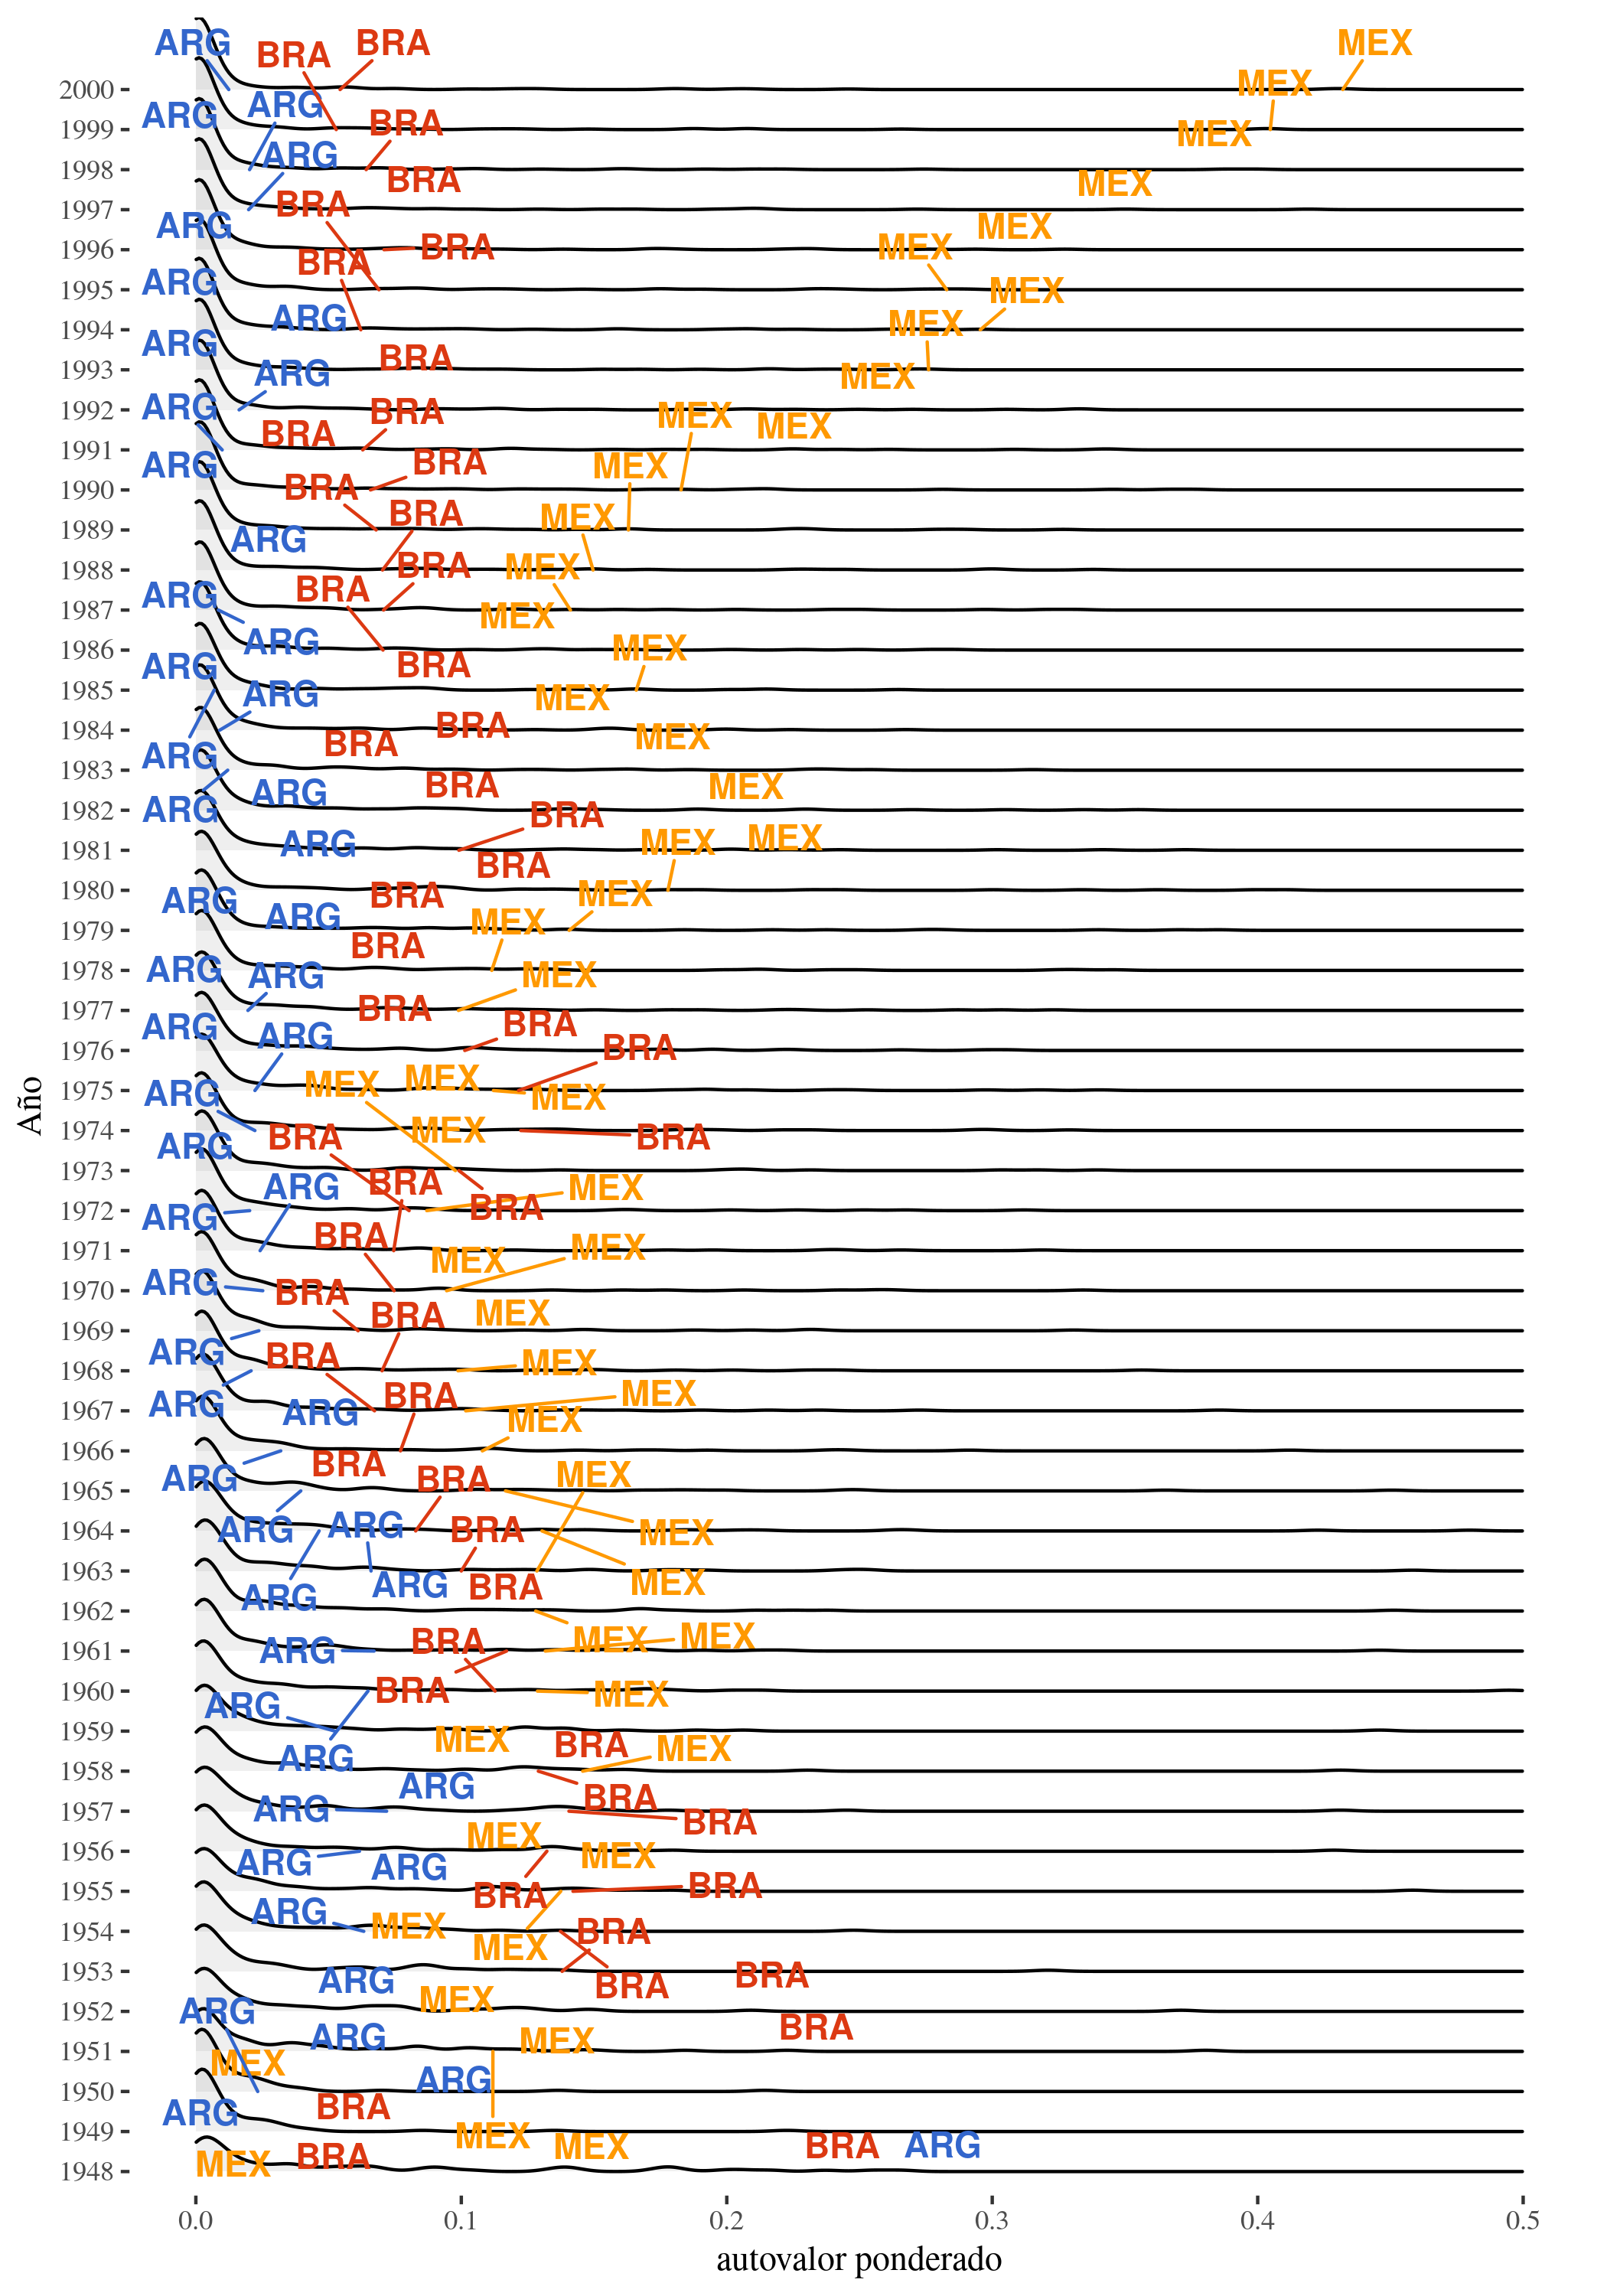
\includegraphics[width=0.7\linewidth]{1950_2000_impo_densidad_ARG_BRA_MEX_atvlrpnd}}
	\caption{Argentina, Brasil y México. Importaciones. Umbral 1\%}
	\label{fig:paises_LP}
\end{figure}


Por último, resulta interesante complementar el análisis de la figura \ref{fig:distribuciones-c}, dónde se veía como China supera a Estados Unidos en ciertas medidas de centralidad para el año 2006, con un análisis de dicha relación en el período de 1948 a 2000. Para ello, en la figura \ref{fig:paises_ASI_LP-a} se observa la distribución de la centralidad de autovalor, y el detalle de estos dos países. \par
En todo el período se observa la predominancia de Estados Unidos como un nodo central del grafo. China, por su parte, comienza en la moda o incluso en la cola izquierda de la distribución. Para luego ubicarse del lado derecho de la misma, entre los sesentas y setentas, aunque aún con valores relativamente bajos. A partir de la década del ochenta, comienza, de forma lenta pero acelerada, a escalar posiciones de mayor centralidad dentro de la red. 
Por su parte, en la figura \ref{fig:paises_ASI_LP-b} se observa la evolución de China junto a Corea y Japón. Aquí se puede ver como no es solo China quién aumenta la centralidad en el grafo, sino Asia en su conjunto. Japón lo hace primero, desde el comienzo de la serie, en los cincuentas, y llega a valores cercanos a 1, el máximo valor posible de esta medida, para los ochentas. Por su parte, Corea también sigue el mismo camino, aunque comienza más tarde, y desde una posición de menor centralidad que los otros países. 

\begin{figure}[h!]
	\centering
	\subfigure[China y Estados Unidos]{\label{fig:paises_ASI_LP-a}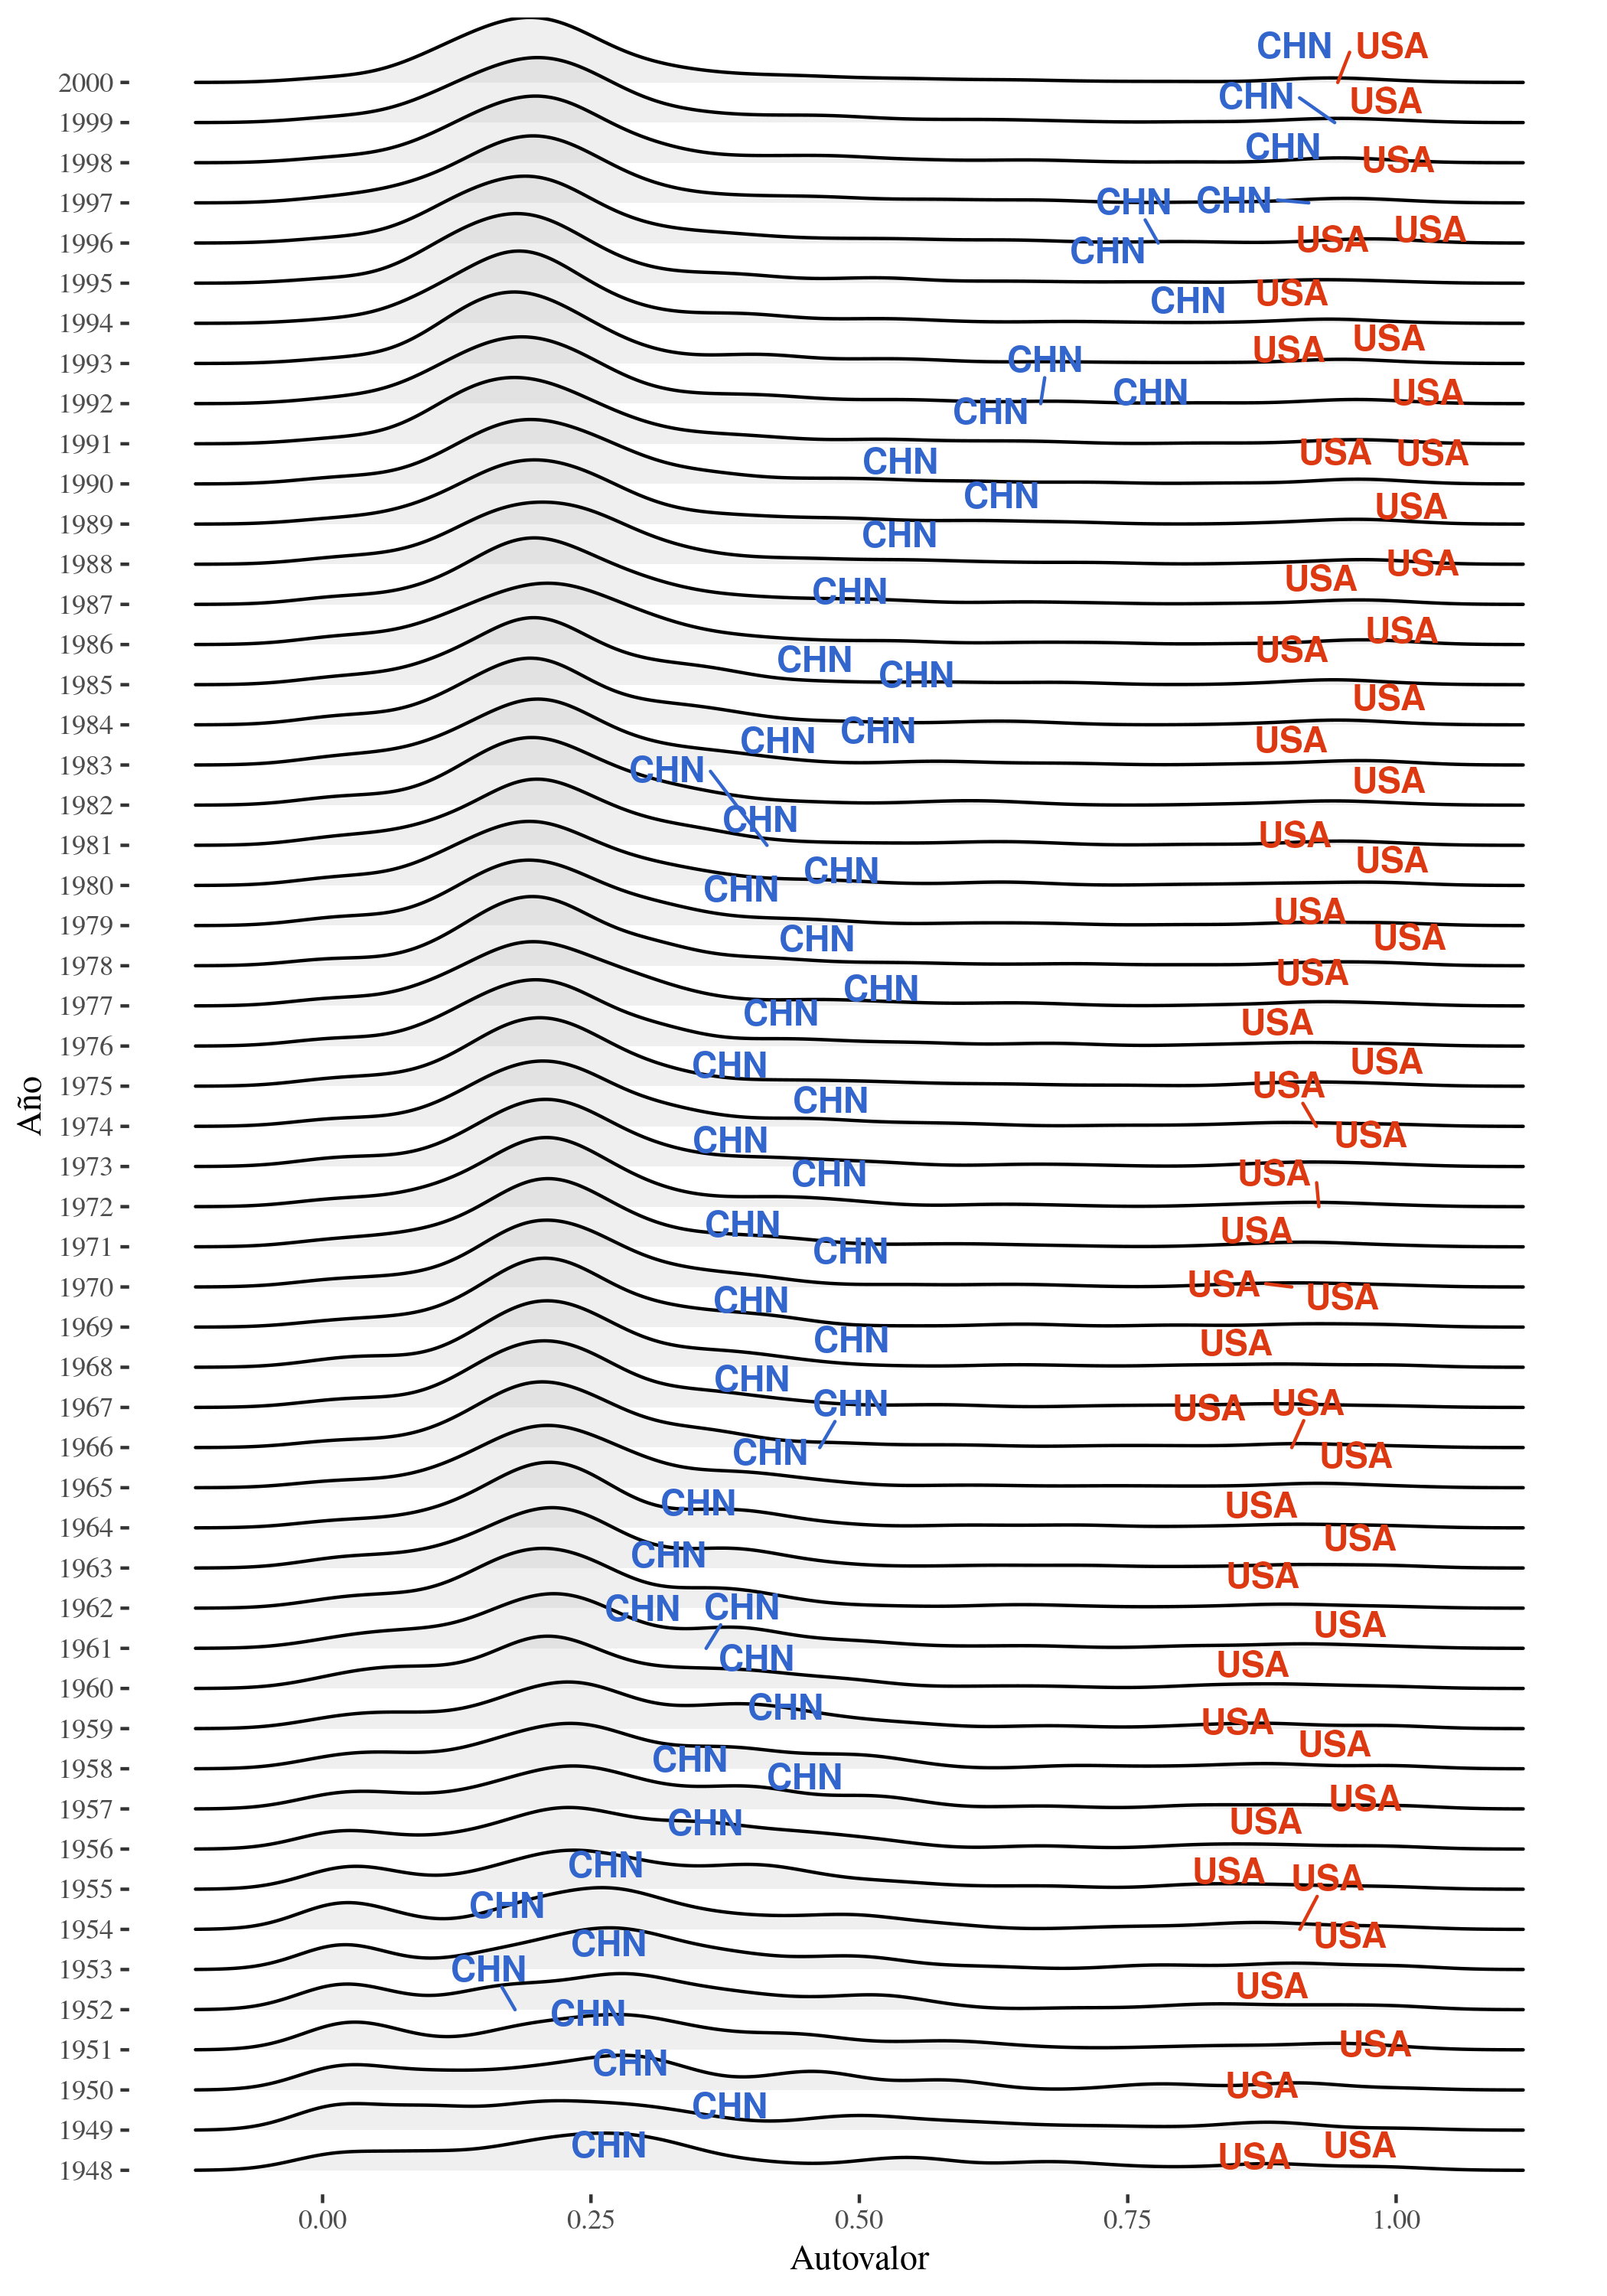
\includegraphics[width=0.7\linewidth]{1950_2000_impo_densidad_USAvsCHN_autovalor_x_yr}}
	\subfigure[Japón,Corea y China]{\label{fig:paises_ASI_LP-b}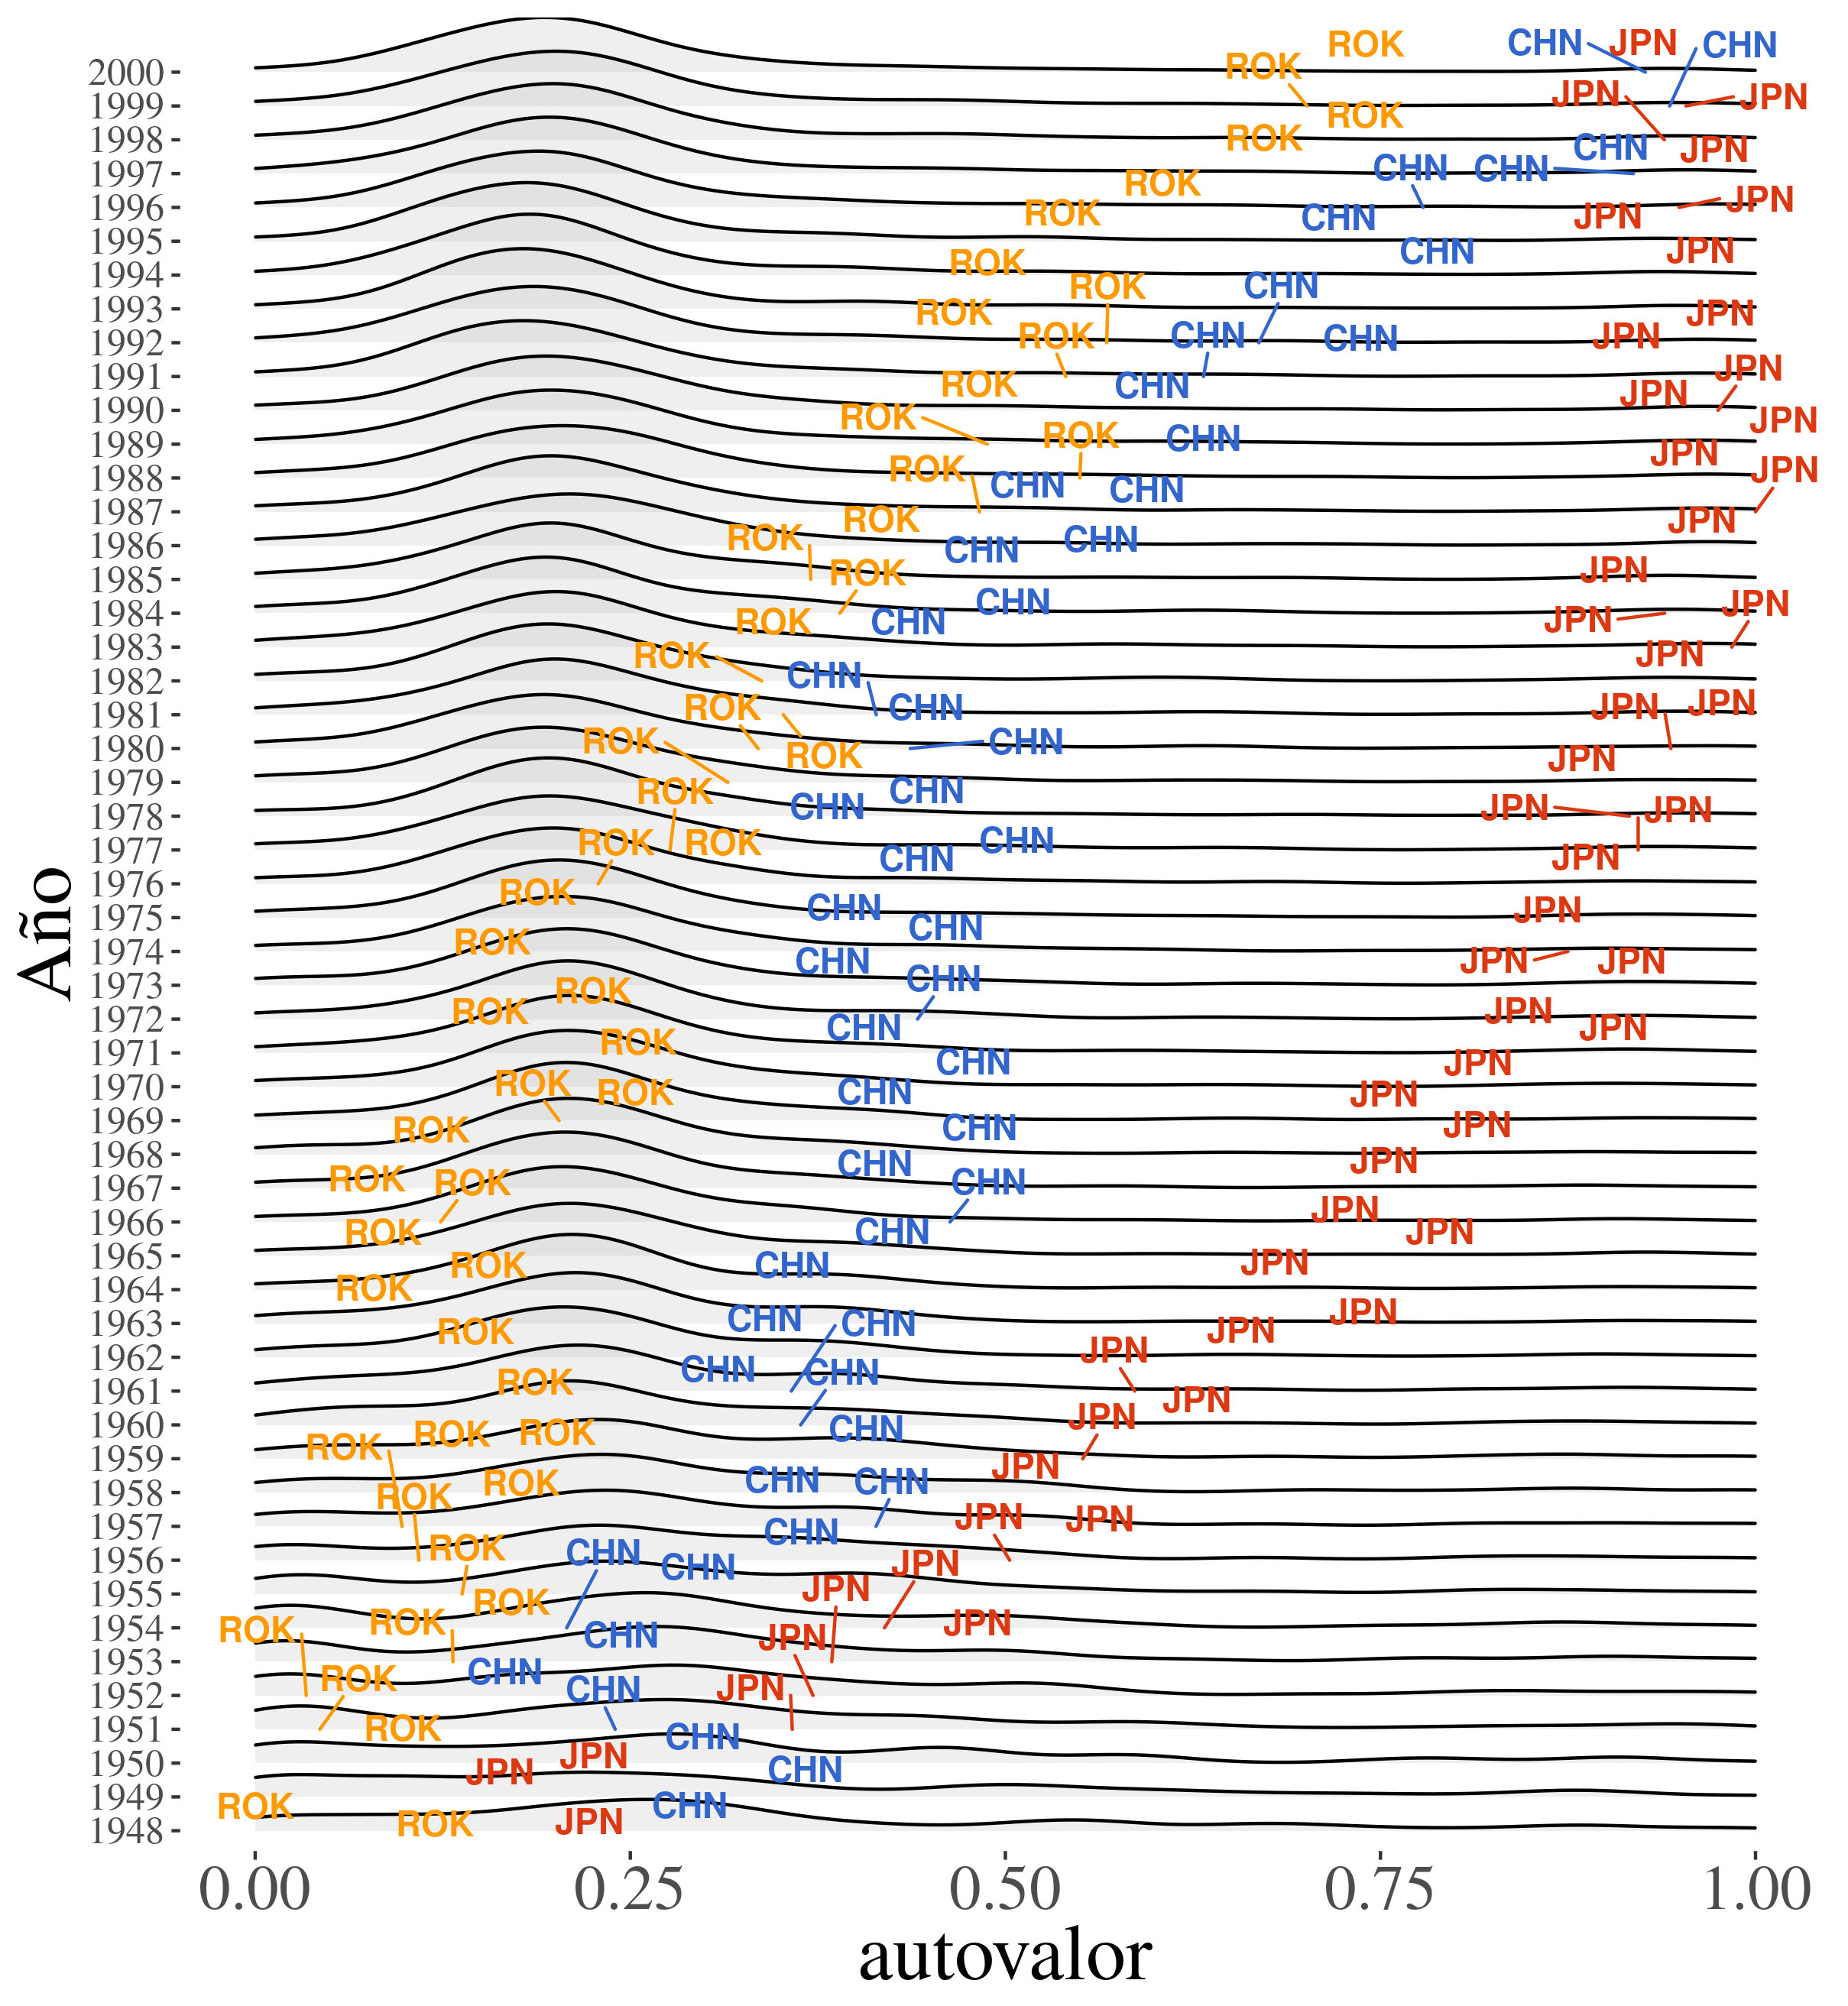
\includegraphics[width=0.7\linewidth]{1950_2000_impo_densidad_CHN_JPN_ROK_atvlr}}
	\caption{Autovalor. Importaciones. Umbral 1\%}
	\label{fig:paises_ASI_LP}
\end{figure}


\section{Conclusiones}

En la presente sección se propuso una primera aproximación de la teoría de grafos como herramienta para la caracterización del comercio internacional, utilizando los datos agregados a nivel país. Para ello se construyó un grafo dirigido no ponderado. Se utilizó al año 2016 como punto de referencia para determinar determinar los mejores hiperparámetros del modelo. En particular, de este análisis resulto que el 1\% constituye un umbral posible para el punto de corte, aunque considerar este hiperparámetro como una dimensión de estudio también permite observar las distintas formas de relación comercial entre los países, y por lo tanto se logra enriquecer la discusión. 

Por su parte, la dimensión temporal en un período de veinte años mostró que las medidas de resumen de un grafo pueden poseer un potencial para la descripción de la crisis del año 2009. El análisis de una serie de largo alcance, por su parte, permite ver los cambios estructurales del comercio internacional.            

Se observó también que la distribución de las medidas de centralidad no pareciera variar en el mediano plazo, aunque sí existe un movimiento visible en los actores principales de la red, lo cual muestra una riqueza en el análisis para describir los cambios de la economía mundial, y los roles cambiantes que en esta juegan los distintos recortes nacionales. 

Finalmente, el trabajo realizado deja una contradicción planteada respecto del rol de ciertos países como consumidores, y de otros como productores, dado que tal estructura no sería sostenible de forma prolongada.


%\bibliographystyle{unsrt}
%\bibliography{bibliografia}
%
\end{document}

